\documentclass[aspectratio=169,handout]{ctexbeamer}
\usepackage{../../../latex/bamboo}
\providetranslation[to=ChineseUTF8]{Example}{例题}
\providetranslation[to=ChineseUTF8]{Solution}{解答}
\definecolor{main}{RGB}{0,0,224}%
\definecolor{second}{RGB}{224,0,0}%
\definecolor{third}{RGB}{112,0,112}%
\definecolor{fourth}{RGB}{0,128,0}%
\definecolor{fifth}{RGB}{255,128,0}%

% Black Theme
% \definecolor{main}{RGB}{0,0,0}%
% \definecolor{second}{RGB}{0,0,0}%
% \definecolor{third}{RGB}{0,0,0}%
% \definecolor{fourth}{RGB}{0,0,0}%
% \definecolor{fifth}{RGB}{0,0,0}%

% Doremi Theme
% \definecolor{main}{RGB}{73,119,213}%
% \definecolor{second}{RGB}{220,60,105}%
% \definecolor{third}{RGB}{122,89,166}%
% \definecolor{fourth}{RGB}{229,143,52}%
% \definecolor{fifth}{RGB}{244,220,10}%

\usepackage{bm}
\usepackage{extarrows}
\usepackage{mathrsfs}
\usepackage{stmaryrd}
\usepackage{multirow}
\usepackage{tikz}
\usepackage{color,calc}
\usepackage{caption}
\usepackage{subcaption}
\usepackage{booktabs}
% \usepackage{wrapfig}
% 文本色
\renewcommand\emph[1]{{\color{main}{\bf #1}}}
\ifcsundef{alert}{
  \newcommand{\alert}[1]{\textcolor{second}{\bf #1}}
}{}
% 非考试内容
\newcommand{\noexer}{\hfill\mdseries\itshape\color{black}\small 非考试内容}
% 枚举数字引用标志
\newcommand\enumnum[1]{{\mdseries\upshape\textcolor{main}{(#1)}}}
% 缩进
\renewcommand{\indent}{\hspace*{1em}}
\setlength{\parindent}{1em}
% 减少公式垂直间距, 配合\endgroup
\newcommand\beqskip[1]{\begingroup\abovedisplayskip=#1\belowdisplayskip=#1\belowdisplayshortskip=#1}

\RequirePackage{tasks}
\settasks{label-format=\textcolor{main},label={(\arabic*)},label-width=1.5em}
% 选择题选项
\NewTasksEnvironment[label={\upshape(\Alph*)},label-width=1.5em]{taskschoice}[()]
% 一行显示多题答案
\NewTasksEnvironment[label={\arabic*.},label-width=1.5em]{tasksans}[()]
% TIKZ 设置
\usetikzlibrary{
	quotes,
	shapes.arrows,
	arrows.meta,
	positioning,
	shapes.geometric,
	overlay-beamer-styles,
	patterns,
	calc,
	angles,
	decorations.pathreplacing,
	backgrounds % 背景边框
}
\tikzset{
	background rectangle/.style={semithick,draw=fourth,fill=white,rounded corners},
  % arrow
	cstra/.style      ={-Stealth},        % right arrow
	cstla/.style      ={Stealth-},        % left arrow
	cstlra/.style     ={Stealth-Stealth}, % left-right arrow
	cstwra/.style     ={-Straight Barb},  % wide ra
	cstwla/.style     ={Straight Barb-},
	cstwlra/.style    ={Straight Barb-Straight Barb},
	cstnra/.style      ={-Latex, line width=0.1cm},
	cstmra/.style      ={-Latex, line width=0.05cm},
	cstmlra/.style     ={Latex-Latex, line width=0.05cm},
	cstaxis/.style        ={-Stealth, thick}, %坐标轴
  % curve
	cstcurve/.style       ={very thick}, %一般曲线
	cstdash/.style        ={thick, dash pattern= on 0.2cm off 0.05cm}, %虚线
  % dot
	cstdot/.style         ={radius=.08}, %实心点
	cstdote/.style        ={radius=.07, fill=white}, %空心点
  % fill
	cstfill/.style       ={fill=black!10},
	cstfille/.style      ={pattern=north east lines, pattern color=black},
	cstfill1/.style       ={fill=main!20},
	cstfille1/.style      ={pattern=north east lines, pattern color=main},
	cstfill2/.style        ={fill=second!20},
	cstfille2/.style       ={pattern=north east lines, pattern color=second},
	cstfill3/.style        ={fill=third!20},
	cstfille3/.style       ={pattern=north east lines, pattern color=third},
	cstfill4/.style        ={fill=fourth!20},
	cstfille4/.style       ={pattern=north east lines, pattern color=fourth},
	cstfill5/.style        ={fill=fifth!20},
	cstfille5/.style       ={pattern=north east lines, pattern color=fifth},
  % node
	cstnode/.style        ={fill=white,draw=black,text=black,rounded corners=0.2cm,line width=1pt},
	cstnode1/.style       ={fill=main!15,draw=main!80,text=black,rounded corners=0.2cm,line width=1pt},
	cstnode2/.style       ={fill=second!15,draw=second!80,text=black,rounded corners=0.2cm,line width=1pt},
	cstnode3/.style       ={fill=third!15,draw=third!80,text=black,rounded corners=0.2cm,line width=1pt},
	cstnode4/.style       ={fill=fourth!15,draw=fourth!80,text=black,rounded corners=0.2cm,line width=1pt},
	cstnode5/.style       ={fill=fifth!15,draw=fifth!80,text=black,rounded corners=0.2cm,line width=1pt}
}
\renewcommand\logo[1]{
	\def\inserttitlegraphic{../../../image/logo/#1.png}
	\def\insertinstitutegraphic{../../../image/logo/#1name.png}
}
\email{zhangshenxing@hfut.edu.cn}
\website{https://zhangshenxing.github.io}
\date{}
\logo{hfut}
\author{张神星}
\institute{合肥工业大学}
\office{翡翠科教楼B1810东}

\RequirePackage[T1]{fontenc}
\setCJKsansfont[ItalicFont={KaiTi},BoldFont={LXGW ZhenKai}]{Source Han Sans HW SC}
\newfontface\cmunrm{cmunrm.otf}\newcommand\cmu[1]{{\cmunrm{#1}}}

\title{线性代数}
\begin{document}
\begin{frame}{课程安排}
\onslide<+->
本课程共$10$周$40$课时, 自2022年9月30日至2022年11月3日. 
\onslide<+->
\emph{课程QQ群}:(入群答案\textbf{1400261B})
\onslide<+->
\begin{itemize}[<*>]
\item 009班(电信工) \emph{\textbf{476993411}}
\item 010班(光信息和智感工) \emph{\textbf{672903188}}
\end{itemize}
\onslide<+->
\emph{教材}:
\begin{tikzpicture}[overlay,xshift=6.5cm,yshift=-1cm]
\draw
	(0,0) node {\includegraphics[height=2.5cm]{misc/book1.jpg}}
	(2.5,0) node {\includegraphics[height=2.5cm]{misc/book2.png}};
\end{tikzpicture}
\begin{itemize}[<*>]
\item 西交高数教研室《复变函数》
\item 张元林《积分变换》
\end{itemize}
\onslide<+->
\emph{成绩构成}:
\begin{itemize}
\item \alert{作业 15\%}, 每章交一次
\item \alert{课堂测验 25\%}, 一共3次,  取最高的两次
\item \alert{期末报告 10\%}
\item \alert{期末考试 50\%}, 至少45分才计算总评
\end{itemize}
\end{frame}


\begin{frame}{复变函数的应用}
\onslide<+->
复变函数的应用非常广泛, 它包括:
\begin{itemize}
\item \emph{数学}中的代数、数论、几何、分析、动力系统……
\item \emph{物理学}中流体力学、材料力学、电磁学、光学、量子力学……
\item \emph{信息学}、\emph{电子学}、\emph{电气工程}……
\end{itemize}

\onslide<+->
可以说复变函数应用之广, 在大学数学课程中仅次于高等数学和线性代数. 
\end{frame}


\begin{frame}{课程内容和学习方法}
\onslide<+->
本课程主要研究下述问题:
\begin{itemize}
\item 复数的由来, 以及复数的基本要素. (\emph{\S~1.1})
\item 复数的运算法则和性质. (\emph{\S\S~1.1-1.3})
\item 复变量函数的定义, 以及与实变量函数的异同点. (\emph{\S\S~1.4-1.6}) 
\item 复变函数的解析性的刻画, 即复变函数的微分理论. (\emph{\S\S~2.1-3.3})
\item 复变函数的积分、级数和留数理论. (\emph{\S\S~3.4-5.3})
\item 积分变换及其应用. (\emph{\S\S~6.1-6.3})
\end{itemize}
\onslide<+->
\begin{center}
\begin{tikzpicture}[node distance=30pt]
\node[cstnodeg,align=center]            (1)  {课前\\预习};
\coordinate[below=of 1] (2);
\node[cstnodeg,align=center,right=of 2] (3)  {认真听课\\记好笔记};
\coordinate[above=of 3] (4);
\node[cstnodeg,align=center,right=of 4] (5)  {课后先阅读\\一遍教材};
\coordinate[below=of 5] (6);
\node[cstnodeg,align=center,right=of 6] (7)  {结合笔记\\汇总知识点};
\coordinate[above=of 7] (8);
\node[cstnodeg,align=center,right=of 8] (9)  {再用作业检\\测学习效果};
\draw[cstnarrow,dcolorc] (1.south) to [bend right] (3.west);
\draw[cstnarrow,dcolorc] (3.north) to [bend left] (5.west);
\draw[cstnarrow,dcolorc] (5.south) to [bend right] (7.west);
\draw[cstnarrow,dcolorc] (7.north) to [bend left] (9.west);
\end{tikzpicture}
\end{center}
\end{frame}



\part{向量和矩阵}
\section{复数及其代数运算}

\subsection{复数的产生}

\begin{frame}{复数的引入\noexer}
	\begin{itemize}
		\item 复数起源于多项式方程的求根问题.
		\item 考虑一元二次方程 $x^2+bx+c=0$.
		\item 配方可得 $\Bigl(x+\dfrac b2\Bigr)^2=\dfrac{b^2-4c}4$.
		\item 于是得到求根公式 $x=\dfrac{-b\pm\sqrt\Delta}2$, 其中 $\Delta=b^2-4c$.
		\begin{enumerate}
			\item 当 $\Delta>0$ 时, 有两个不同的实根;
			\item 当 $\Delta=0$ 时, 有一个二重的实根;
			\item 当 $\Delta<0$ 时, 无实根.
		\end{enumerate}
		\item 可以看出, 在一元二次方程中, 我们可以舍去包含\alert{负数开方}的解.
		\item 然而在一元三次方程中, 即便只考虑实数根也会不可避免地引入负数开方.
	\end{itemize}
\end{frame}



\begin{frame}{三次方程的根\noexer}
	\onslide<+->
	\begin{example}[nearnext]
		解方程 $x^3+6x-20=0$.
	\end{example}
	\onslide<+->
	\begin{solution}[nearprev,sidepic,righthand width=3.2cm,leftupper=0mm]
		\begin{itemize}
			\item 设 $x=u+v$,
			\item 那么 $u^3+v^3+3uv(u+v)+6(u+v)-20=0$.
			\item 我们希望 $u^3+v^3=20$, $uv=-2$.
			\item 那么 $u^3,v^3$ 满足一元二次方程 $X^2-20X-8=0$.
			\item 解得 $u^3=10\pm\sqrt{108}=(1\pm\sqrt3)^3$.
			\item 所以 $u=1\pm\sqrt3$, $v=1\mp\sqrt 3$.
			\item $x=u+v=2$.
		\end{itemize}
		\tcblower
		\onslide<+->{
		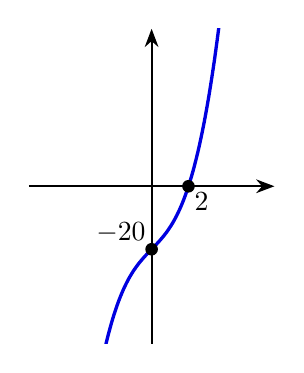
\begin{tikzpicture}
			\begin{scope}[xscale=.78]
				\draw[cstaxis] (-2,0)--(2,0);
				\draw[cstaxis] (0,-2)--(0,2);
				\clip (-2,-2) rectangle (2,2);
				\begin{scope}[xscale=.3,yscale=.04]
					\draw[cstcurve,main,domain=-3:4,smooth] plot (\x,{\x*\x*\x+6*\x-20});
					\coordinate (A) at (2,0);
					\coordinate (B) at (0,-20);
				\end{scope}
				\draw[inner sep=2pt]
					(A) node[below right] {$2$}
					(B) node[above left] {$-20$};
			\end{scope}
			\begin{scope}[cstdot]
				\fill (A) circle;
				\fill (B) circle;
			\end{scope}
		\end{tikzpicture}}
	\end{solution}
\end{frame}


\begin{frame}{三次方程的根\noexer}
	\beqskip{1pt}
	\onslide<+->
	\begin{example}[nearnext]
		解方程 $x^3-7x+6=0$.
	\end{example}
	\onslide<+->
	\begin{solution}[nearprev,sidepic,righthand width=2.7cm,leftupper=0mm]
		\begin{itemize}
			\item 类似地 $x=u+v$, 其中 $u^3+v^3=-6$, $uv=\frac73$.
			\item 于是 $u^3,v^3$ 满足一元二次方程 $X^2+6X+\frac{343}{27}=0$.
			\item 这个方程没有实数解, 我们可以强行解得 
		\end{itemize}
		\onslide<+->{%
		\[
			u^3=-3+\dfrac{10}9\sqrt{-3},\ 
			\visible<+->{u=\frac{3+2\sqrt{-3}}3,\frac{-9+\sqrt{-3}}6,\frac{3-5\sqrt{-3}}6,}
		\]}
		\begin{itemize}
			\item $v=\dfrac{3-2\sqrt{-3}}3,\dfrac{-9-\sqrt{-3}}6,\dfrac{3+5\sqrt{-3}}6$,
			\item $x=u+v=2,-3,1$.
		\end{itemize}
		\tcblower
		\onslide<+->{%
		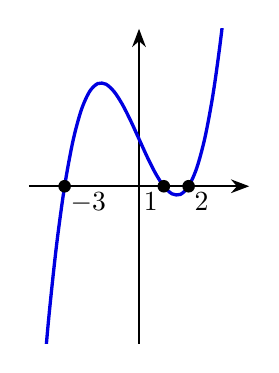
\begin{tikzpicture}
			\begin{scope}[xscale=.7]
				\def\a{-3}
				\def\b{1}
				\def\c{2}
				\draw[cstaxis] (-2,0)--(2,0);
				\draw[cstaxis] (0,-2)--(0,2);
				\clip (-2,-2) rectangle (2,2);
				\begin{scope}[xscale=.45,yscale=.1]
					\draw[cstcurve,main,domain=-4:4,smooth] plot (\x,{(\x-\a)*(\x-\b)*(\x-\c)});
					\coordinate (A) at (\a,0);
					\coordinate (B) at (\b,0);
					\coordinate (C) at (\c,0);
				\end{scope}
				\draw[inner sep=2pt]
					(A) node[below right] {$-3$}
					(B) node[below left] {$1$}
					(C) node[below right] {$2$};
			\end{scope}
			\begin{scope}[cstdot]
				\fill (A) circle;
				\fill (B) circle;
				\fill (C) circle;
			\end{scope}
		\end{tikzpicture}}
	\end{solution}
	\endgroup
\end{frame}


\begin{frame}{三次方程的根\noexer}
	\begin{itemize}
		\item 一般地, 方程 $x^3+px+q=0$ 的解为($p=0$ 情形较简单, 这里不考虑)
		\[
			x=u-\frac p{3u},\quad u^3=-\frac q2+\sqrt{\Delta},\quad \Delta=\frac{q^2}4+\frac{p^3}{27}.
		\]
		\item 通过分析函数图像的极值点可以知道:
	\end{itemize}
	\begin{center}
		\begin{tikzpicture}[visible on=<3->]
			\begin{scope}[scale=.65,
				declare function={
					f(\x)=\x*\x*\x-3*\x;
				}
			]
				\def\a{2.5}
				\draw[cstaxis] (-2,0)--(2,0);
				\draw[cstaxis] (0,-2) node[below] {$\Delta>0$, 有 $1$ 个根}--(0,2);
				\clip (-2,-2) rectangle (2,2);
				\begin{scope}[xscale=.35,yscale=.1]
					\draw[cstcurve,main,domain=-3:4,smooth] plot (\x,{f(\x)-f(\a)});
					\coordinate (A) at (\a,0);
				\end{scope}
			\end{scope}
			\fill[cstdot] (A) circle;
			\begin{scope}[visible on=<4->,xshift=5cm]
				\begin{scope}[scale=.65]
					\def\a{-2}
					\def\b{1}
					\draw[cstaxis] (-2,0)--(2,0);
					\draw[cstaxis] (0,-2) node[below,align=center] {$\Delta=0$, 有 $2$ 个根\\$x=-\sqrt[3]{4q},\half\sqrt[3]{4q}$ ($2$重).}--(0,2);
					\clip (-2,-2) rectangle (2,2);
					\begin{scope}[xscale=.35,yscale=.1]
						\draw[cstcurve,main,domain=-4:3,smooth] plot ({\x},{(\x-\a)*(\x-\b)*(\x-\b)});
						\coordinate (A) at (\a,0);
						\coordinate (B) at (\b,0);
					\end{scope}
				\end{scope}
				\begin{scope}[cstdot]
					\fill (A) circle;
					\fill (B) circle;
				\end{scope}
			\end{scope}
			\begin{scope}[visible on=<5->,xshift=10cm]
				\begin{scope}[scale=.65]
					\def\a{-3}
					\def\b{.5}
					\def\c{2.5}
					\draw[cstaxis] (-2,0)--(2,0);
					\draw[cstaxis] (0,-2) node[below] {$\Delta<0$, 有 $3$ 个根}--(0,2);
					\clip (-2,-2) rectangle (2,2);
					\begin{scope}[xscale=.3,yscale=.05]
						\draw[cstcurve,main,domain=-5:5,smooth] plot ({\x},{(\x-\a)*(\x-\b)*(\x-\c)});
						\coordinate (A) at (\a,0);
						\coordinate (B) at (\b,0);
						\coordinate (C) at (\c,0);
					\end{scope}
				\end{scope}
				\begin{scope}[cstdot]
					\fill (A) circle;
					\fill (B) circle;
					\fill (C) circle;
				\end{scope}
			\end{scope}
		\end{tikzpicture}
	\end{center}
\end{frame}


\begin{frame}{三次方程的根\noexer}
	\begin{itemize}
		\item 由此可见, 若想使用求根公式, 就\alert{必须接受负数开方}.
		\item 那么为什么当 $\Delta<0$ 时, 从求根公式一定能得到 $3$ 个实根呢?
		\item 这个问题在我们学习了第一章的内容之后可以得到回答.
		\item 尽管在十六世纪, 人们已经得到了三次方程的求根公式, 然而对其中出现的虚数, 却是难以接受.
		\item 莱布尼兹曾说: {\color{third}\itshape 圣灵在分析的奇观中找到了超凡的显示, 这就是那个理想世界的端兆, 那个介于存在与不存在之间的两栖物, 那个我们称之为虚的 $-1$ 的平方根。}
		\item 不过, 现在我们可以用更为现代和严格的语言来引入复数.
	\end{itemize}
\end{frame}

\subsection{复数的概念}

\begin{frame}{复数的定义}
	\begin{itemize}
		\item 现在我们来正式介绍复数的概念.
		\item 为了避免记号 $\sqrt{-1}$ 带来的歧义, 我们先引入抽象符号 $\ii$, 再通过定义它的运算来构造复数.
	\end{itemize}
	\onslide<+->
	\begin{definition}
		固定一个记号 $\ii$, \emph{复数}就是形如 $z=x+y\ii$ 的元素, 其中 $x,y$ 均是实数, 且不同的 $(x,y)$ 对应不同的复数.
	\end{definition}
	\begin{itemize}
		\item 实数 $x$ 可以自然地看成复数 $x+0\ii$.
	\end{itemize}
\end{frame}


\begin{frame}{复平面}
	\begin{itemize}
		\item 回忆全体实数、有理数、整数、自然数构成的集合分别记作 $\BR,\BQ,\BZ,\BN$.
		\item 将\emph{全体复数记作 $\BC$}.
		\item 那么 $\BC$ 自然构成一个二维实线性空间, 且 $\{1,\ii\}$ 是一组基. 
		\item 因此它和平面上的点可以建立一一对应, 并将建立起这种对应的平面称为\emph{复平面}.
	\end{itemize}
	\onslide<+->
	\begin{center}
		\begin{tikzpicture}
			\begin{scope}
				\draw[cstaxis] (-.5,0)--(3,0);
				\draw[cstaxis] (0,-.5)--(0,2.5);
				\coordinate [label=below left:$0$] (O) at (0,0);
				\coordinate [label=above:\textcolor{second}{$z=x+y\ii$}] (A) at (2,1.5);
				\coordinate (B) at (2,0);
				\coordinate (C) at (0,1.5);
				\draw[cstdash] (B)--(A)--(C);
				\fill[cstdot,second] (A) circle;
				\draw[third,Latex-Latex,line width=.5mm] (2.8,1)--(4,1) node[midway,below,third] {一一对应};
			\end{scope}
			\begin{scope}[xshift=5cm]
				\coordinate [label=below left:$O$] (O) at (0,0);
				\coordinate [label=above:\textcolor{second}{$Z(x,y)$}] (A) at (2,1.5);
				\coordinate (B) at (2,0);
				\coordinate (C) at (0,1.5);
				\draw[cstdash] (B)--(A)--(C);
				\fill[cstdot,second] (A) circle;
				\draw[decorate,decoration={brace,amplitude=5},main,cstfill1] (O)--(B) node[midway,above=2mm] {$x$};
				\draw[decorate,decoration={brace,amplitude=5},main,cstfill1] (C)--(O) node[midway,right=2mm] {$y$};
				\draw[third,Latex-Latex,line width=.5mm] (2.8,1)--(4,1) node[midway,below,third] {一一对应};
				\draw[cstaxis] (-.5,0)--(3,0);
				\draw[cstaxis] (0,-.5)--(0,2.5);
			\end{scope}
			\begin{scope}[xshift=10cm]
				\draw[cstaxis] (-.5,0)--(3,0);
				\draw[cstaxis] (0,-.5)--(0,2.5);
				\coordinate [label=below left:$O$] (O) at (0,0);
				\coordinate [label=above:\textcolor{second}{$\overrightarrow{OZ}=(x,y)$}] (A) at (2,1.5);
				\draw[cstcurve,cstra,second] (O)--(A);
			\end{scope}
		\end{tikzpicture}
	\end{center}
\end{frame}


\begin{frame}{实部和虚部, 虚数和纯虚数}
	\onslide<+->
	\begin{itemize}
		\item $x,y$ 轴分别对应复平面的\emph{实轴}和\alert{虚轴}.
		\item 称 $z=x+y\ii$ 中 $x=\Re z$ 为 $z$ 的\emph{实部}; $y=\Im z$ 为 $z$ 的\alert{虚部}.
		\item 当虚部 $\Im z=0$ 时, $z$ 为实数, 它落在实轴上.
		\item 不是实数的复数是\textcolor{third}{\bf 虚数}.
		\item 当实部 $\Re z=0$ 且 \alert{$z\neq0$} 时, $z$ 为\alert{纯虚数}, 它落在虚轴上.
	\end{itemize}
	\onslide<1->
	\begin{figure}[hbpt]
		\centering
		\begin{minipage}{.48\textwidth}
			\raggedleft
			\begin{tikzpicture}
				\coordinate [label=below left:$0$] (O) at (0,0);
				\coordinate (B) at (2,0);
				\coordinate (C) at (0,1.5);
				\draw[cstaxis] (-.5,0)--(3,0);
				\draw[cstaxis] (0,-.5)--(0,2.5);
				\begin{scope}[visible on=<3->]
					\draw[decorate,decoration={brace,amplitude=5},main,cstfill1] (B)--(O) node[midway,below=1.5mm] {$\Re z$};
					\draw[decorate,decoration={brace,amplitude=5},second,cstfill2] (C)--(O) node[midway,right=1.5mm] {$\Im z$};
					\coordinate [label=above:\textcolor{third}{$z=x+y\ii$}] (A) at (2,1.5);
					\draw[cstdash] (B)--(A)--(C);
					\fill[cstdot,third] (A) circle;
				\end{scope}
				\begin{scope}[visible on=<2->]
					\coordinate [label=above:\textcolor{main}{实轴}] (R) at (3,0);
					\coordinate [label=right:\textcolor{second}{虚轴}] (I) at (0,2.5);
					\draw[cstaxis,main] (-.5,0)--(R);
					\draw[cstaxis,second] (0,-.5)--(I);
				\end{scope}
				\draw[main,->,thick,visible on=<4->] (-2,.2)-|(.6,0);
				\draw[second,->,thick,visible on=<6->] (-2,1.3)--(0,1.3);
				\draw 
					(-2,.1) node[cstnode,draw=main,text=main,visible on=<4->] {实数}
					(-2,1.2) node[align=center,cstnode,draw=second,text=second,visible on=<6->] {纯虚数\\不含原点};
			\end{tikzpicture}
		\end{minipage}
		\begin{minipage}{.48\textwidth}
			\centering
			\begin{tikzpicture}
				\filldraw[cstcurve,cstfill] (.8,0) circle (2.6 and 2);
				\coordinate (R) at (0,-.8);
				\filldraw[cstcurve,main,fill=white,visible on=<4->] (R) circle (1.2 and .7);
				\coordinate (I) at (0,.8);
				\draw (R) node[align=center,main,visible on=<4->] {实数 \\$0,1,\sqrt2,\pi,\ee$};
				\draw (I) node[align=center,second,visible on=<6->] {纯虚数 \\$\ii,-\ii ,\pi\ii$};
				\draw[cstcurve,second,visible on=<6->] (I) circle (1.2 and .7);
				\draw 
					(3.7,0) node[align=center] {全\\体\\复\\数}
					(2,0) node[align=center,third,visible on=<5->] {虚数 \\$\ii,\pi\ii,\frac{-1+\sqrt 3 \ii}2$};
			\end{tikzpicture}
		\end{minipage}
	\end{figure}
\end{frame}


\begin{frame}{例题:判断实数和纯虚数}
	\onslide<+->
	\begin{example}[nearnext]
		实数 $x$ 取何值时, $z=(x^2+3x-4)+(x^2+5x-6)\ii$ 是:
		\begin{subexample}[2]
			\item 实数;
			\item 纯虚数.
		\end{subexample}
	\end{example}
	\onslide<+->
	\begin{solution}[nearprev]
		\begin{enumerate}
			\item $\Im z=x^2+5x-6=0$, 即 $x=1$ 或 $-6$.
			\item $\Re z=x^2+3x-4=0$, 即 $x=1$ 或 $-4$.
				\onslide<+->{%
					但同时要求 $\Im z=x^2+5x-6\neq 0$, 因此 $x\neq 1$.
				}\onslide<+->{%
					故 $x=-4$.
				}
		\end{enumerate}
	\end{solution}
	\onslide<+->
	\begin{exercise}
		若 $x^2(1+\ii)-x(5+4\ii)+4+3\ii$ 是纯虚数, 则实数 $x=$\fillblankframe{$4$}.
	\end{exercise}
\end{frame}


\subsection{复数的代数运算}


\begin{frame}{复数的加法与减法}
	\begin{itemize}
		\item 设 $z_1=x_1+y_1\ii,z_2=x_2+y_2\ii$.
		\item 定义复数的\emph{加法}和\emph{减法}:
		\[
			z_1+z_2=(x_1+x_2)+(y_1+y_2)\ii,\quad
			z_1-z_2=(x_1-x_2)+(y_1-y_2)\ii.
		\]
		\item 复数的加减法与其对应的向量 $\overrightarrow{OZ}$ 的加减法是一致的.
	\end{itemize}
	\onslide<1->
	\begin{center}
		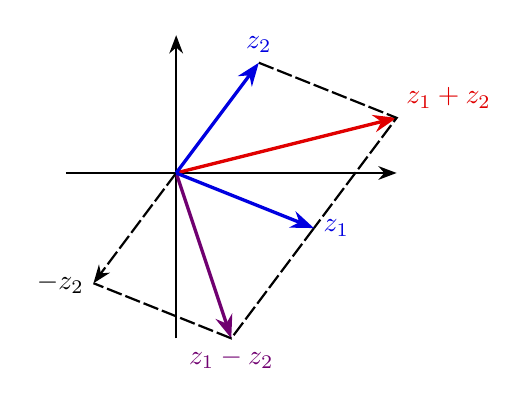
\begin{tikzpicture}[scale=.7]
			\draw[cstaxis] (-2,0)--(4,0);
			\draw[cstaxis] (0,-3)--(0,2.5);
			\coordinate (O) at (0,0);
			\coordinate [label=right:\textcolor{main}{$z_1$}] (Z1) at (2.5,-1);
			\coordinate [label=above:\textcolor{main}{$z_2$}] (Z2) at (1.5,2);
			\begin{scope}[visible on=<3->]
				\coordinate [label=above right:\textcolor{second}{$z_1+z_2$}] (P) at ($(Z1)+(Z2)$);
				\draw[cstcurve,cstra,second] (O)--(P);
				\draw[cstdash] (Z2)--(P)--(Z1);
			\end{scope}
			\begin{scope}[visible on=<4->]
				\coordinate [label=below:\textcolor{third}{$z_1-z_2$}] (M) at ($(Z1)-(Z2)$);
				\coordinate [label=left:{$-z_2$}] (neg) at ($(O)-(Z2)$);
				\draw[cstcurve,cstra,third] (O)--(M);
				\draw[cstdash,cstra] (O)--(neg);
				\draw[cstdash] (Z1)--(M)--(neg);
			\end{scope}
			\draw[cstcurve,cstra,main] (O)--(Z1);
			\draw[cstcurve,cstra,main] (O)--(Z2);
		\end{tikzpicture}
	\end{center}
\end{frame}


\begin{frame}{复数的乘除法}
	\begin{itemize}
		\item \alert{规定 $\ii\cdot \ii=-1$}.
		\item 定义复数的\emph{乘法}:
		\begin{align*}
			z_1\cdot z_2&
			=(x_1+y_1\ii)(x_2+y_2\ii)
			=x_1\cdot x_2+x_1\cdot y_2\ii+y_1\ii\cdot x_2+y_1\ii\cdot y_2\ii\\
			&=(x_1x_2-y_1y_2)+(x_1y_2+x_2y_1)\ii.
		\end{align*}
		\item 此时加法/乘法交换律, 结合律以及乘法分配律均成立.
		\item 待定系数可得复数的\emph{除法}定义为:
		\[
			\frac{z_1}{z_2}
			=\frac{(x_1+y_1\ii)(x_2-y_2\ii)}{x_2^2+y_2^2}
			=\frac{x_1x_2+y_1y_2}{x_2^2+y_2^2}+\frac{x_2y_1-x_1y_2}{x_2^2+y_2^2}\ii.
		\]
		\item 对于正整数 $n$, 定义 $z$ 的 \emph{$n$ 次幂}为 $n$ 个 $z$ 相乘.
		\item 当 $z\neq 0$ 时, 还可以定义 $z^0=1,z^{-n}=\dfrac1{z^n}$.
	\end{itemize}
\end{frame}


\begin{frame}{例: 单位根}
	\onslide<+->
	\begin{example}
		\begin{enumerate}
			\item $\ii^2=-1,\ii^3=-\ii ,\ii^4=1$.
			\onslide<+->{%
			一般地, 对于整数 $n$, 
			\[
				\ii^{4n}=1,\quad \ii^{4n+1}=i,\quad
				\ii^{4n+2}=-1,\quad \ii^{4n+3}=-\ii.
			\]
			}
			\vspace{-\baselineskip}
			\item 令 $\omega=\dfrac{-1+\sqrt 3\ii}2$, 则 $\omega^2=\dfrac{-1-\sqrt3\ii}2,\omega^3=1$.
			\item 令 $z=1+\ii$, \onslide<+->{则
			\[
				z^2=2\ii,\quad z^3=-2+2\ii,\quad z^4=-4,\quad z^8=16=2^4.
			\]}
		\end{enumerate}
		\bigdel\bigdel
	\end{example}
	\begin{itemize}
		\item 将满足 $z^n=1$ 的复数 $z$ 称为 \emph{$n$ 次单位根}.
		\item 那么 $1,\ii,-1,-\ii $ 是 $4$ 次单位根, $1,\omega,\omega^2$ 是 $3$ 次单位根, $-\omega$ 是 $6$ 次单位根.
	\end{itemize}
\end{frame}


\begin{frame}{例: 代数式的计算}
	\begin{itemize}
		\item 实数情形的等差数列求和公式、等比数列求和公式、二项式展开、平方差公式等在复数情形也成立.
	\end{itemize}
	\onslide<+->
	\begin{example}[nearnext]
		化简 $1+\ii+\ii^2+\dots+\ii^{1000}$.
	\end{example}
	\onslide<+->
	\begin{solution}[nearprev]
		根据等比数列求和公式, $1+\ii+\ii^2+\dots+\ii^{1000}
			=\dfrac{\ii^{1001}-1}{\ii-1}
			\visible<+->{=\dfrac{\ii-1}{\ii-1}=1.}$
	\end{solution}
	\onslide<+->
	\begin{exercise}
		化简 $\Bigl(\dfrac{1+\ii}{1-\ii}\Bigr)^{2026}$=\fillblankframe{$-1$}.
	\end{exercise}
\end{frame}


\subsection{共轭复数}


\begin{frame}{共轭复数的定义}
	\onslide<+->
	\begin{definition}
		称 $z$ 在复平面关于实轴的对称点为它的\emph{共轭复数 $\ov z$}.
		换言之, $\ov{x+y\ii}=x-y\ii$.
	\end{definition}
	\onslide<+->
	\begin{exercise}
		$z$ 关于虚轴的对称点是\fillblankframe{$-\ov z$}.
	\end{exercise}
\end{frame}

\begin{frame}{共轭复数的性质}
	\begin{itemize}
		\item 从定义出发, 不难验证共轭复数满足如下性质:
		\begin{enumerate}\bf
			\item $z$ 是 $\ov z$ 的共轭复数.\hfill\alert{共轭是一种对合}
			\item $\ov{z_1\pm z_2}=\ov{z_1}\pm\ov{z_2},\ 
			\ov{z_1\cdot z_2}=\ov{z_1}\cdot\ov{z_2},\ 
			\ov{\Bigl(\dfrac{z_1}{z_2}\Bigr)}=\dfrac{~\ov{z_1}~}{~\ov{z_2}~}$.
			\hfill \alert{共轭复数和四则运算交换}
			\item $z\ov{z}=(\Re z)^2+(\Im z)^2$.
			\item $z+\ov z=2\Re z,\ z-\ov z=2\ii\Im z$.
			\hfill \alert{$x,y$ 和 $z,\ov z$ 可相互表示}
			\item $z=\ov z\iff z$ 是实数; $z=-\ov z\iff z$ 是纯虚数或 $z=0$.\hfill\alert{判断实数和纯虚数}
		\end{enumerate}
		\item 这些性质意味着使用共轭复数进行计算和证明,往往比直接使用 $x,y$ 表达的形式更简单.
	\end{itemize}
\end{frame}


\begin{frame}{例题:共轭复数证明等式}
	\onslide<+->
	\begin{example}
		证明 $z_1\cdot\ov{z_2}-\ov{z_1}\cdot z_2=2\ii\Im(z_1\cdot\ov{z_2})$.
	\end{example}
	\onslide<+->
	我们可以设 $z_1=x_1+y_1\ii,z_2=x_2+y_2\ii$, 然后代入等式两边化简并比较实部和虚部得到.
	\onslide<+->
	但我们利用共轭复数可以更简单地证明它.
	\onslide<+->
	\begin{proof}[leftupper=0mm]
		\begin{itemize}
			\item 由于 $\ov{z_1\cdot\ov{z_2}}=\ov{z_1}\cdot\ov{\ov{z_2}}=\ov{z_1}\cdot z_2$, 
			\item 因此
			\[
				z_1\cdot\ov{z_2}-\ov{z_1}\cdot z_2
				=z_1\cdot\ov{z_2}-\ov{z_1\cdot\ov{z_2}}
				=2\ii\Im(z_1\cdot\ov{z_2}).\qedhere
			\]
		\end{itemize}
	\end{proof}
\end{frame}


\begin{frame}{例题:共轭复数判断实数}
	\onslide<+->
	\begin{example}[nearnext]
		设 $z=x+y\ii$ 是虚数.
		证明: $x^2+y^2=1$ 当且仅当 $z+\dfrac 1z$ 是实数.
	\end{example}
	\onslide<+->
	\begin{proof}[nearprev,leftupper=0mm]
		\begin{itemize}
			\item $z+\dfrac 1z$ 是实数等价于
				$z+\dfrac 1z=\ov{\Bigl(z+\dfrac 1z\Bigr)}=\ov z+\dfrac1{~\ov z~}$,
			\item 等价于
			\[
				z-\ov z=\frac1{~\ov z~}-\frac1z=\frac{z-\ov z}{z\ov z},\quad (z-\ov z)(z\ov z-1)=0.
			\]
			\item 由 $z$ 是虚数可知 $z\neq \ov z$.
			\item 故上述等式等价于 $z\ov z=1$, 即 $x^2+y^2=1$.\qedhere
		\end{itemize}
	\end{proof}
\end{frame}


\begin{frame}{例: 复数的代数计算}
	\onslide<+->
	由于 $z\ov z$ 是一个实数,
	\onslide<+->
	因此在做复数的除法运算时, 可以利用下式将其转化为乘法:
	\[
		\dfrac{z_1}{z_2}=\dfrac{z_1\ov{z_2}}{z_2\ov{z_2}}=\dfrac{z_1\ov{z_2}}{x_2^2+y_2^2}.
	\]
	\bigdel
	\onslide<+->
	\begin{example}[nearnext]
		$z=-\dfrac1\ii-\dfrac{3\ii}{1-\ii }$, 求 $\Re z,\Im z$ 以及 $z\ov z$.
	\end{example}
	\onslide<+->
	\begin{solution}[nearprev]
		\[
			z=-\frac1\ii-\frac{3\ii}{1-\ii }
			\onslide<+->{=\ii-\frac{3\ii-3}2=\frac32-\half \ii,}
		\]
		\onslide<+->{%
		\[
			\Re z=\frac32,\quad\Im z=-\half ,\quad
			z\ov z=\Bigl(\frac32\Bigr)^2+\Bigl(-\half\Bigr)^2=\frac52.
		\]
		}
		\bigdel
	\end{solution}
\end{frame}


\begin{frame}{例: 复数的代数计算}
	\onslide<+->
	\begin{example}[nearnext]
		设 $z_1=5-5\ii,z_2=-3+4\ii$, 求 $\ov{\Bigl(\dfrac{z_1}{z_2}\Bigr)}$.
	\end{example}
	\onslide<+->
	\begin{solution}[nearprev]
		\begin{align*}
			\frac{z_1}{z_2}&=\frac{5-5\ii}{-3+4\ii}
			\onslide<+->{=\frac{(5-5\ii)(-3-4\ii)}{(-3)^2+4^2}}\\
			&\onslide<+->{=\frac{(-15-20)+(-20+15)\ii}{25}}
			\onslide<+->{=-\frac75-\frac15\ii,}
		\end{align*}
		\onslide<+->{%
			因此 $\ov{\Bigl(\dfrac{z_1}{z_2}\Bigr)}=-\dfrac75+\dfrac15\ii$.
		}
	\end{solution}
\end{frame}



% \begin{frame}{复数域\noexer}
% 	\begin{itemize}
% 		\item 复数全体构成一个\emph{域}.
% 		\item 所谓的域, 是指带有如下内容和性质的集合
% 		\begin{itemize}\bf
% 			\item 包含 $0,1$, 且有四则运算;
% 			\item 满足加法结合/交换律, 乘法结合/交换/分配律;
% 			\item 对任意 $a$, $a+0=a\times 1=a$.
% 		\end{itemize}
% 		\item 有理数全体 $\BQ$, 实数全体 $\BR$ 也构成域, 它们是 $\BC$ 的子域.
% 		\item 与有理数域和实数域有着本质不同的是, 复数域是\emph{代数闭域}:
% 		\item 对于任何次数 $n\ge 1$ 的复系数多项式
% 		\[
% 			p(z)=z^n+c_{n-1}z^{n-1}+\cdots+c_1z+c_0,
% 		\]
% 		都存在复数 $z_0$ 使得 $p(z_0)=0$.
% 		\item 由此不难知道, 复系数多项式可以因式分解成一次多项式的乘积.
% 		\item 我们会在第五章证明该结论.
% 	\end{itemize}
% \end{frame}


% \begin{frame}{复数域不是有序域\noexer}
% 	\begin{itemize}
% 		\item \onslide<+->
% 	\end{itemize}
% 	在 $\BQ,\BR$ 上可以定义出一个好的大小关系,
% 	\onslide<+->
% 	换言之它们是有序域, 即存在一个满足下述性质的 $>$:
% 	\begin{itemize}\bf
% 		\item 若 $a\neq b$, 则要么 $a>b$, 要么 $b>a$;
% 		\item 若 $a>b$, 则对于任意 $c$, $a+c>b+c$;
% 		\item 若 $a>b,c>0$, 则 $ac>bc$.
% 	\end{itemize}
% 	\onslide<+->
% 	而 \alert{$\BC$ 却不是有序域}.
% 	\onslide<+->
% 	若 $\ii>0$, 则
% 	\[
% 		-1=\ii\cdot \ii>0,\quad -\ii =-1\cdot \ii>0.
% 	\]
% 	\onslide<+->
% 	于是 $0>\ii$, 矛盾! 同理 $\ii<0$ 也不可能.
% \end{frame}

\section{复数的三角与指数形式}

\subsection{复数的模和辐角}
\begin{frame}{复数的极坐标形式}
	\onslide<+->
	由平面的极坐标表示, 我们可以得到复数的另一种表示方式.
	\onslide<+->
	以 $0$ 为极点, 正实轴为极轴, 逆时针为极角方向可以自然定义出复平面上的极坐标系.
	\onslide<+->
	\begin{center}
		\begin{minipage}{.4\textwidth}
			\centering
			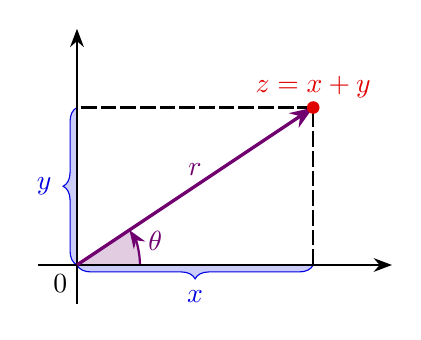
\begin{tikzpicture}
				\coordinate [label=below left:$0$] (O) at (0,0);
				\coordinate [label=above:\textcolor{second}{$z=x+y\ii$}] (Z) at (3,2);
				\coordinate (X) at (3,0);
				\coordinate (Y) at (0,2);
				\draw[decorate,decoration={brace,amplitude=5},main,cstfill1] (X)--(O) node[midway,below=2mm] {$x$};
				\draw[decorate,decoration={brace,amplitude=5},main,cstfill1] (O)--(Y) node[midway,left=2mm] {$y$};
				\draw[third,thick,cstra] pic [cstfill3,draw=third, "$\theta$", angle eccentricity=1.3, angle radius=0.8cm] {angle=X--O--Z};
				\draw[cstaxis] (-.5,0)--(4,0);
				\draw[cstaxis] (0,-.5)--(0,3);
				\draw[cstcurve,third,cstra] (O)--(Z) node[midway,above,third] {$r$};
				\draw[cstdash] (X)--(Z)--(Y);
				\fill[cstdot,second] (Z) circle;
			\end{tikzpicture}
		\end{minipage}
		\begin{minipage}{.56\textwidth}
			\centering
			\onslide<4->{
			\[ x=r\cos\theta,\qquad y=r\sin\theta,
	\]
			\[r=\sqrt{x^2+y^2},\qquad \theta=\arctan\dfrac yx\text{ 或 }\arctan\dfrac yx\pm\pi.\]}
		\end{minipage}
	\end{center}
	\vspace{-\baselineskip}

	\onslide<+->
	\onslide<+->
	\begin{definition}
		\begin{itemize}
			\item 称 $r$ 为 $z$ 的\emph{模}, 记为 \emph{$|z|=r$}.
			\item 称 $\theta$ 为 $z$ 的\emph{辐角}, 记为 \emph{$\Arg z=\theta$}.
			\onslide<+->{约定 \alert{$0$ 的辐角没有定义}.}
		\end{itemize}
	\end{definition}
\end{frame}


\begin{frame}{辐角主值}
	\onslide<+->
	任意 $z\neq 0$ 的辐角有无穷多个.
	\onslide<+->
	我们固定选择其中位于 $(-\pi,\pi]$ 的那个, 并称之为\emph{辐角主值}或\emph{辐角主值}, 记作 $\emphm{\arg z}$.
	\onslide<+->
	那么 $\emphm{\Arg z=\arg z+2k\pi, k\in\BZ}$.

	\onslide<2->
	\begin{figure}[hbpt]
		\centering
		\begin{minipage}{.46\textwidth}
			\onslide<4->{
			\[\arg z=\begin{cases}
				\visible<4->{\emphn{\arctan\dfrac yx,}}&\visible<4->{\emphn{x>0;}}\vspace{1ex}\\
				\visible<5->{\alertn{\arctan\dfrac yx+\pi,}}&\visible<5->{\alertn{x<0,y\ge0;}}\vspace{1ex}\\
				\visible<6->{\color{third}{\arctan\dfrac yx-\pi,}}&\visible<6->{\color{third}{x<0,y<0;}}\\
				\visible<7->{\color{fourth}{\dfrac\pi2,}}&
				\visible<7->{\color{fourth}{x=0,y>0;}}\\
				\visible<7->{\color{fourth}{-\dfrac\pi2,}}&
				\visible<7->{\color{fourth}{x=0,y<0.}}
				\end{cases}\]}
		\end{minipage}
		\begin{minipage}{.52\textwidth}
			\begin{tikzpicture}
				\draw[cstaxis](-2.5,0)->(2.5,0); 
				\draw[cstaxis](0,-2)->(0,2);
				\draw[cstaxis,main,cstwla] (-1.5,0) arc(180:-180:1.5);
				\filldraw[cstdote,draw=main] (-1.5,-.07) circle;
				\begin{scope}[visible on=<4->]
					\coordinate [label=above:\textcolor{main}{$0$}] (A) at (1.7,0);
					\fill[cstdot,main] (A) circle;
					\coordinate [label=above right:\textcolor{main}{$\arctan\dfrac yx$}] (B) at (.9,.9);
					\fill[cstdot,main] (B) circle;
					\coordinate [label=right:\textcolor{main}{$\arctan\dfrac yx$}] (C) at (1.4,-.9);
					\fill[cstdot,main] (C) circle;
				\end{scope}
				\begin{scope}[visible on=<5->]
					\coordinate [label=above left:\textcolor{second}{$\arctan\dfrac yx+\pi$}] (D) at (-1.1,.8);
					\fill[cstdot,second] (D) circle;
					\coordinate [label=below:\textcolor{second}{$\pi$}] (E) at (-.9,0);
					\fill[cstdot,second] (E) circle;
				\end{scope}
				\begin{scope}[visible on=<6->]
					\coordinate [label=left:\textcolor{third}{$\arctan\dfrac yx-\pi$}] (F) at (-1.6,-.7);
					\fill[cstdot,third] (F) circle;
				\end{scope}
				\begin{scope}[visible on=<7->]
					\coordinate [label=left:\textcolor{fourth}{$\dfrac\pi2$}] (G) at (0,.5);
					\fill[cstdot,fourth] (G) circle;
					\coordinate [label=right:\textcolor{fourth}{$-\dfrac\pi2$}] (H) at (0,-.6);
					\fill[cstdot,fourth] (H) circle;
				\end{scope}
			\end{tikzpicture}
		\end{minipage}
	\end{figure}
	\vspace{-\baselineskip}
	\onslide<9->
	注意 \alert{$\arg \ov z=-\arg z$ 未必成立}, 仅当 $z$ 不是负实数和 $0$ 时成立.
\end{frame}


\begin{frame}{复数模的性质}\small
	\onslide<+->
	复数的模满足如下性质:
	\begin{figure}[hbpt]
		\centering
		\begin{minipage}{.48\textwidth}
			\begin{itemize}\bf
				\item $z\ov z=|z|^2=|\ov z|^2$;
				\item $\abs{\Re z},\abs{\Im z}\le |z|\le\abs{\Re z}+\abs{\Im z}$;
			\end{itemize}
		\end{minipage}
		\begin{minipage}{.48\textwidth}
			\begin{itemize}\bf
				\item $\big||z_1|-|z_2|\big|\le|z_1\pm z_2|\le|z_1|+|z_2|$;
				\item $|z_1+z_2+\cdots+z_n|\le|z_1|+|z_2|+\cdots+|z_n|$.
			\end{itemize}
		\end{minipage}
	\end{figure}
	\begin{center}
		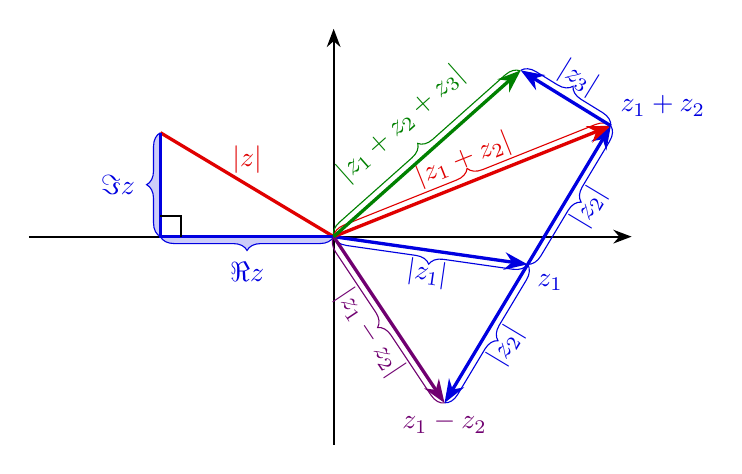
\begin{tikzpicture}[visible on=<3->,scale=.88]
			\draw[cstaxis] (-4.4,0)--(4.3,0);
			\draw[cstaxis] (0,-3)--(0,3);
			\coordinate (O) at (0,0);
			\coordinate (Z) at (-2.5,1.5);
			\coordinate (R) at (-2.5,0);
			\draw[decorate,decoration={brace,amplitude=5},main,cstfill1] (O)--(R) node[midway,below=2mm,main] {$\abs{\Re z}$};
			\draw[decorate,decoration={brace,amplitude=5},main,cstfill1] (R)--(Z) node[midway,left=2mm,main] {$\abs{\Im z}$};
			\draw[cstcurve,second] (O)--(Z) node[midway,above,second] {$|z|$};
			\draw[cstcurve,main] (Z)--(R)--(O);
			\draw[thick] (R) ++(0,.3)--++(.3,0)--++(0,-.3);
	
			\begin{scope}[visible on=<4->]
				\coordinate [label=below right:\textcolor{main}{$z_1$}] (Z1) at (2.8,-.4);
				\coordinate (Z2) at (1.2,2);
				\coordinate [label=above right:\textcolor{main}{$z_1+z_2$}] (P) at ($(Z1)+(Z2)$);
				\coordinate [label=below:\textcolor{third}{$z_1-z_2$}] (M) at ($(Z1)-(Z2)$);
				\draw[decorate,decoration={brace,amplitude=5},main] (Z1)--(O) node[midway,below,sloped] {$|z_1|$};
				\draw[decorate,decoration={brace,amplitude=5},main] (P)--(Z1) node[midway,below,sloped] {$|z_2|$};
				\draw[decorate,decoration={brace,amplitude=5},second] (O)--(P) node[midway,above,sloped] {$|z_1+z_2|$};
				\draw[decorate,decoration={brace,amplitude=5},main] (Z1)--(M) node[midway,below,sloped] {$|z_2|$};
				\draw[decorate,decoration={brace,amplitude=5},third] (M)--(O) node[midway,below,sloped] {$|z_1-z_2|$};
				\begin{scope}[cstcurve,cstra]
					\draw[main] (O)--(Z1);
					\draw[main] (Z1)--(P);
					\draw[second] (O)--(P);
					\draw[third] (O)--(M);
					\draw[main] (Z1)--(M);
				\end{scope}
			\end{scope}

			\begin{scope}[visible on=<5->]
				\coordinate (A) at (2.7,2.4);
				\draw[decorate,decoration={brace,amplitude=5},main] (A)--(P) node[midway,above,sloped] {$|z_3|$};
				\draw[decorate,decoration={brace,amplitude=5},fourth] (O)--(A) node[midway,above=2mm,sloped] {$|z_1+z_2+z_3|$};
				\begin{scope}[cstcurve,cstra]
					\draw[main] (P)--(A);
					\draw[fourth] (O)--(A);
				\end{scope}
			\end{scope}
		\end{tikzpicture}
	\end{center}
\end{frame}


\begin{frame}{例题:共轭复数解决模的等式}
	\beqskip{0pt}
	\onslide<+->
	\begin{example}
		证明
		\begin{enumerate}
			\item $|z_1z_2|=|z_1\ov{z_2}|=|z_1|\cdot|z_2|$;
			\item $|z_1+z_2|^2=|z_1|^2+|z_2|^2+2\Re(z_1\ov{z_2})$.
		\end{enumerate}
	\end{example}

	\onslide<+->
	\begin{proof}
		\begin{enumerate}
			\item 因为
				\[|z_1z_2|^2=z_1z_2\cdot\ov{z_1}\ov{z_2}
				=z_1z_2\ov{z_1}\ov{z_2}=|z_1|^2\cdot|z_2|^2,
	\]
				\onslide<+->{%
					所以 $|z_1z_2|=|z_1|\cdot|z_2|$.
				}\onslide<+->{%
					因此 $|z_1\ov{z_2}|=|z_1|\cdot|\ov{z_2}|=|z_1|\cdot|z_2|$.
				}
			\item 因为
				\begin{align*}
					\text{左边}&=(z_1+z_2)(\ov{z_1}+\ov{z_2})
					=z_1\ov{z_1}+z_2\ov{z_2}+z_1\ov{z_2}+\ov{z_1}z_2,\\
					\text{右边}&=z_1\ov{z_1}+z_2\ov{z_2}+z_1\ov{z_2}+\ov{z_1\ov{z_2}},
				\end{align*}
				\onslide<+->{%
					而 $\ov{z_1\ov{z_2}}=\ov{z_1}z_2$, 所以两侧相等.\qedhere
				}
		\end{enumerate}
	\end{proof}
	\endgroup
\end{frame}


\subsection{复数的三角形式和指数形式}
\begin{frame}{复数的三角形式和指数形式}
	\onslide<+->
	由 $x=r\cos\theta,y=r\sin\theta$ 可得
	\onslide<+->
	\begin{definition}[复数的三角形式]
	\[
		z=r(\cos\theta+\ii\sin\theta).\]	
	\end{definition}
	\onslide<+->
	定义 \alert{$\ee^{\ii\theta}=\exp(\ii\theta):=\cos\theta+\ii\sin\theta$} (欧拉恒等式),
	\onslide<+->
	则我们得到
	\begin{definition}[复数的指数形式]
	\[
		z=r\ee^{\ii\theta}=r\exp(\ii\theta).
	\]
	\end{definition}
	\onslide<+->
	这两种形式的等价的, 指数形式可以认为是三角形式的一种缩写方式.

	\onslide<+->
	求复数的三角和指数形式的\alert{关键在于计算模和辐角}.
\end{frame}


\begin{frame}{例: 求复数的三角和指数形式}
	\onslide<+->
	\begin{example}
		将 $z=-\sqrt{12}-2\ii$ 化成三角形式和指数形式.
	\end{example}

	\onslide<+->
	\begin{solution}
		$r=|z|=\sqrt{12+4}=4$.
		\onslide<+->{%
			由于 $z$ 在第三象限,
		}\onslide<+->{%
			因此
			\[\arg z=\arctan\frac{-2}{-\sqrt{12}}-\pi=\frac\pi6-\pi=-\frac{5\pi}6.
	\]
		}\onslide<+->{%
			故
			\[z=4\left[\cos\Bigl(-\frac{5\pi}6\Bigr)+\ii\sin\Bigl(-
			\frac{5\pi}6\Bigr)\right]=4\ee^{-\frac{5\pi\ii}6}.
	\]
		}
	\end{solution}
\end{frame}


\begin{frame}{例: 求复数的三角和指数形式}
	\beqskip{0pt}
	\onslide<+->
	\begin{example}
		将 $z=\sin\dfrac\pi5+\ii\cos\dfrac\pi5$ 化成三角形式和指数形式.
	\end{example}
	\onslide<+->
	\begin{solution}
		$r=|z|=1$.
		\onslide<+->{%
		由于 $z$ 在第一象限, 因此
		\[\arg z=\arctan\frac{\cos(\pi/5)}{\sin(\pi/5)}=\arctan\cot\frac\pi 5=\frac\pi2-\frac\pi5=\frac{3\pi}{10}.
		\]}\onslide<+->{%
		故
		\[
			z=\cos\frac{3\pi}{10}+\ii\sin\frac{3\pi}{10}=\ee^{\frac{3\pi\ii}{10}}.
		\]}
	\end{solution}
	\onslide<+->
	\begin{solution}[另解]
		\[
			z=\sin\frac\pi5+\ii\cos\frac\pi5
			\visible<+->{=\cos\Bigl(\frac\pi2-\frac\pi5\Bigr)+\ii\sin\Bigl(\frac\pi2-\frac\pi5\Bigr)}
			\visible<+->{=\cos\frac{3\pi}{10}+\ii\sin\frac{3\pi}{10}=\ee^{\frac{3\pi\ii}{10}}.}
		\]
	\end{solution}
	\endgroup
\end{frame}


\begin{frame}{例: 求复数的三角和指数形式}
	\onslide<+->
	求复数的三角或指数形式时, 我们只需要任取一个辐角就可以了, 不要求必须是辐角主值.

	\onslide<+->
	\begin{exercise}
		将 $z=\sqrt 3-3\ii$ 化成三角形式和指数形式.
	\end{exercise}

	\onslide<+->
	\begin{answer}
		$\displaystyle z=2\sqrt3\Bigl(\cos\frac{-\pi}3+\ii\sin\frac{-\pi}3\Bigr)
		=2\sqrt3\ee^{-\frac{\pi\ii}3}$, 写成 $\dfrac{5\pi}3$ 也可以.
	\end{answer}
\end{frame}


\begin{frame}{模为 $1$ 的复数}
	\onslide<+->
	两个模相等的复数之和的三角和指数形式形式较为简单.
	\onslide<+->
	\[
		\ee^{\ii\theta}+\ee^{\ii\varphi}
		=2\cos\frac{\theta-\varphi}2\ee^{\frac{\theta+\varphi}2\ii}.
	\]
	\vspace{-\baselineskip}
	\onslide<+->
	\begin{center}
		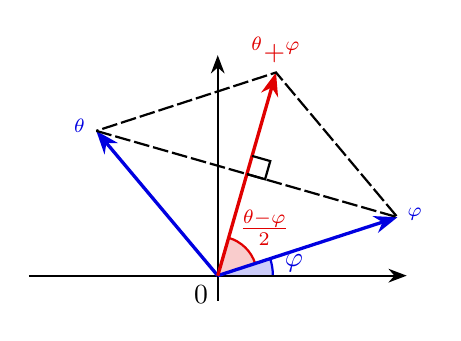
\begin{tikzpicture}[scale=.8]
			\coordinate [label=below left:0] (O) at (0,0);
			\coordinate [label=right:\textcolor{main}{$\ee^{\ii\varphi}$}] (Z1) at ({3*cos(18)},{3*sin(18)});
			\coordinate [label=left:\textcolor{main}{$\ee^{\ii\theta}$}] (Z2) at ({3*cos(130)},{3*sin(130)});
			\coordinate [label=above:\textcolor{second}{$\ee^{\ii\theta}+\ee^{\ii\varphi}$}] (P) at ($(Z1)+(Z2)$);
			\coordinate (M) at ($0.5*(P)$);
			\coordinate (X) at (2,0);
			\draw[thick,main] pic [cstfill1, draw=main,"$\varphi$", angle eccentricity=1.4, angle radius=0.7cm] {angle=X--O--Z1};
			\draw[thick,second] pic [cstfill2, draw=second, "$\frac{\theta-\varphi}2$", angle eccentricity=1.7] {angle=Z1--O--P};
			\draw[cstaxis] (-3,0)--(3,0);
			\draw[cstaxis] (0,-.4)--(0,3.5);
			\draw[cstcurve,cstra,main] (O)--(Z1);
			\draw[cstcurve,cstra,main] (O)--(Z2);
			\draw[cstcurve,cstra,second] (O)--(P);
			\draw[cstdash] (Z2)--(Z1)--(P)--(Z2);
			\draw[thick] (M)--++({.3*cos(16)},{-.3*sin(16)})--++({.3*sin(16)},{.3*cos(16)})--++({-.3*cos(16)},{.3*sin(16)});
		\end{tikzpicture}
	\end{center}
	\onslide<+->
	\begin{example}
		如果 $|z|=1,\arg z=\theta$, 则 $z+1=2\cos\dfrac\theta2 \ee^{\frac{\theta \ii}2}$.
	\end{example}
\end{frame}

\section{方阵的行列式}

\subsection{行列式的定义}

\begin{frame}{引例: 平行四边形的面积\noexer}
	\onslide<+->
	设平面上有 $\parallelogram OACB$, 其中 $A,B$ 坐标分别为 $\bfu=(a,b)^\rmT, \bfv=(c,d)^\rmT$.
\onslide<+->{%
		如果 $\bfu=(1,0)^\rmT,\bfv=(0,1)^\rmT$, 那么面积为 $1$.
	}\onslide<+->{%
		如果将 $\bfu$ 换成 $k\bfu$, 那么面积变为 $|k|$ 倍.
	}\onslide<+->{%
		如果将 $\bfu$ 拆分为 $(a,0)^\rmT+(0,b)^\rmT$, 那么得到的三个平行四边形的面积有什么联系呢?
	}
	\begin{center}
	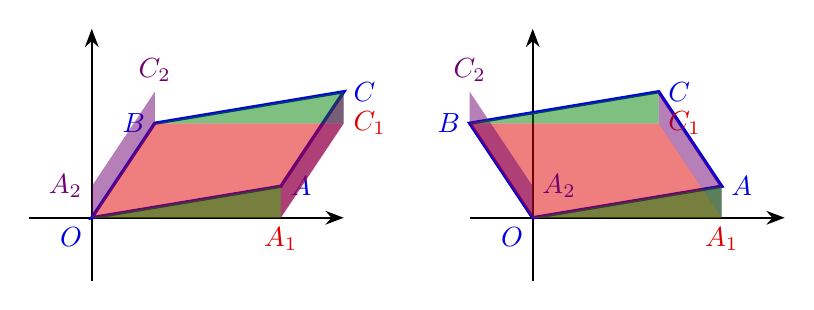
\begin{tikzpicture}[scale=.8]
		\begin{scope}
			\draw[cstaxis] (-1,0)--(4,0);
			\draw[cstaxis] (0,-1)--(0,3);
			\draw[cstcurve,main] (0,0)--(3,0.5)--(4,2)--(1,1.5)--cycle;
			\draw (0,0) node[main,below left] {$O$};
			\draw (3,0.5) node[main,right] {$A$};
			\draw (1,1.5) node[main,left]{$B$};
			\draw (4,2) node[main,right] {$C$};
			\fill[cstcurve,second,fill opacity=.5,visible on=<5->] (0,0)--(3,0)--(4,1.5)--(1,1.5)--cycle;
			\begin{scope}[visible on=<5->]
				\draw (3,0) node[second,below] {$A_1$};
				\draw (4,1.5) node[second,right] {$C_1$};
			\end{scope}
			\fill[cstcurve,third,fill opacity=.5,visible on=<6->] (0,0)--(0,0.5)--(1,2)--(1,1.5)--cycle;
			\begin{scope}[visible on=<6->]
				\draw (0,.5) node[third,left] {$A_2$};
				\draw (1,2) node[third,above] {$C_2$};
			\end{scope}
			\fill[cstcurve,fourth,fill opacity=.5,visible on=<8->] (1,1.5)--(4,1.5)--(4,2)--cycle;
			\fill[cstcurve,fourth,fill opacity=.5,visible on=<9->] (0,0)--(3,0)--(3,0.5)--cycle;
			\fill[cstcurve,third,fill opacity=.5,visible on=<10->] (3,0)--(3,0.5)--(4,2)--(4,1.5)--cycle;
		\end{scope}

		\begin{scope}[xshift=7cm,visible on=<11->]
			\draw[cstaxis] (-1,0)--(4,0);
			\draw[cstaxis] (0,-1)--(0,3);
			\draw[cstcurve,main] (0,0)--(3,0.5)--(2,2)--(-1,1.5)--cycle;
			\draw (0,0) node[main,below left] {$O$};
			\draw (3,0.5) node[main,right] {$A$};
			\draw (-1,1.5) node[main,left]{$B$};
			\draw (2,2) node[main,right] {$C$};
			\fill[cstcurve,second,fill opacity=.5,visible on=<12->] (0,0)--(3,0)--(2,1.5)--(-1,1.5)--cycle;
			\fill[cstcurve,third,fill opacity=.5,visible on=<12->] (0,0)--(0,0.5)--(-1,2)--(-1,1.5)--cycle;
			\begin{scope}[visible on=<12->]
				\draw (3,0) node[second,below] {$A_1$};
				\draw (2,1.5) node[second,right] {$C_1$};
				\draw (0,.5) node[third,right] {$A_2$};
				\draw (-1,2) node[third,above] {$C_2$};
			\end{scope}
			\fill[cstcurve,third,fill opacity=.5,visible on=<13->] (3,0)--(3,0.5)--(2,2)--(2,1.5)--cycle;
			\fill[cstcurve,fourth,fill opacity=.5,visible on=<13->] (0,0)--(3,0)--(3,0.5)--cycle;
			\fill[cstcurve,fourth,fill opacity=.5,visible on=<14->] (-1,1.5)--(2,1.5)--(2,2)--cycle;
		\end{scope}
	\end{tikzpicture}
	\end{center}
	\onslide<+->
	令 $A_1(a,0)$, 并作 $\parallelogram OA_1C_1B$;
	\onslide<+->
	令 $A_2(0,b)$, 并作 $\parallelogram OA_2C_2B$.
	\onslide<+->
	那么 $\parallelogram OACB$ 的面积是这两个相加还是相减?
	\onslide<+->\onslide<+->\onslide<+->
	使用割补法可知为\alert{二者相减}.
	
	\onslide<+->
	如果 $A$ 在第一象限, $B$ 在第二象限.
	\onslide<+->
	那么 $\parallelogram OACB$ 的面积是这两个相加还是相减?\onslide<+->\onslide<+->
	使用割补法可知为\alert{二者相加}.
\end{frame}


\begin{frame}{有向面积\noexer}
	\onslide<+->
	为何第一种情形是相减而第二种情形是相加呢?
	\onslide<+->
	观察发现: 这些平行四边形中只有第一种情形的 $\parallelogram OA_2C_2B$, 从 $OA_2$ 到 $OB$ 是顺时针方向.
	\onslide<+->
	如果定义\emph{有向面积}并记为
	\[|\bfu,\bfv|=\begin{vmatrix}
		a&c\\b&d
	\end{vmatrix}=\begin{cases}
		S_{\parallelogram OACB},&\text{从 $OA$ 到 $OB$ 是逆时针};\\
		-S_{\parallelogram OACB},&\text{从 $OA$ 到 $OB$ 是顺时针}.
	\end{cases}\]
	\onslide<+->
	那么
	\[\begin{vmatrix}
		a&c\\b&d
	\end{vmatrix}=\begin{vmatrix}
		a&c\\0&d
	\end{vmatrix}+\begin{vmatrix}
		0&c\\b&d
	\end{vmatrix}=a\begin{vmatrix}
		1&c\\0&d
	\end{vmatrix}+b\begin{vmatrix}
		0&c\\1&d
	\end{vmatrix}.\]
	\onslide<+->
	换言之, $\bfv$ 固定时, 则 $|\bfu,\bfv|$ 关于 $\bfu$ 是线性的.
	\onslide<+->
	同理, $\bfu$ 固定时, $|\bfu,\bfv|$ 关于 $\bfv$ 也是线性的.
\end{frame}


\begin{frame}{平行多面体情形\noexer}
	\onslide<+->
	将上述概念推广到 $n$ 维情形.
	\onslide<+->
	考虑 $n$ 维空间中由从原点出发的向量 $\bfv_1,\dots,\bfv_n$ 张成的平行多面体.
	\onslide<+->
	如果 $\bfv_1,\dots,\bfv_n$ 就是按顺序各个分量上的单位向量
	\[\bfe_1=(1,0,\dots,0)^\rmT,\quad
	\bfe_2=(0,1,\dots,0)^\rmT,\quad\cdots,\quad
	\bfe_n=(0,0,\dots,1)^\rmT,\]
	则有向面积为 $1$.
	\onslide<+->
	如果交换 $\bfv_i,\bfv_j$ 的位置, 有向面积相差 $-1$ 倍.
	\onslide<+->
	于是得到 $n$ 维情形的有向面积 $|\bfv_1,\dots,\bfv_n|$ 应当满足:
	\begin{enumerate}
		\item $|\bfe_1,\dots,\bfe_n|=1$;
		\item 反对称性: $|\cdots,\bfv_i,\cdots,\bfv_j,\cdots|=-|\cdots,\bfv_j,\cdots,\bfv_i,\cdots|$;
		\item $|\cdots,k\bma,\cdots|=k|\cdots,\bma,\cdots|$;
		\item $|\cdots,\bma+\bmb,\cdots|=|\cdots,\bma,\cdots|+|\cdots,\bmb,\cdots|$.
	\end{enumerate}
\end{frame}


\begin{frame}{行列式的定义\noexer}
	\onslide<+->
	设 $n$ 阶方阵 $\bfA=(a_{ij})$ 的各列形成的向量为 $\bfv_1,\dots,\bfv_n$,
	\onslide<+->
	称有向面积 $|\bfv_1,\cdots,\bfv_n|$ 就是方阵 $\bfA$ 的\emph{行列式}.
	\onslide<+->
	注意到
	\[\bfv_j=a_{1j}\bfe_1+a_{2j}\bfe_2+\cdots+a_{nj}\bfe_n,\]
	\onslide<+->
	利用线性性质将行列式展开将会得到 $n^n$ 项
	\[\sum_{k_1,k_2,\dots,k_n=1}^n|\bfe_{k_1},\cdots,\bfe_{k_n}| a_{k_11}a_{k_22}\cdots a_{k_nn}.\]

	\onslide<+->
	如果 $k_i=k_j$, 则交换 $\bfe_{k_i},\bfe_{k_j}$ 可知 $|\bfe_{k_1},\cdots,\bfe_{k_n}|=0$.
	\onslide<+->
	从而只剩下 $k_1,k_2,\dots,k_n$ 是 $1,2,\dots,n$ 的排列时的那些项.
	\onslide<+->
	例如: 
	\begin{align*}
		\begin{vmatrix}
			a_{11}&a_{12}\\
			a_{21}&a_{22}
		\end{vmatrix}&=|a_{11}\bfe_1,a_{12}\bfe_1+a_{22}\bfe_2|+|a_{21}\bfe_2,a_{12}\bfe_1+a_{22}\bfe_2|\\
		&=a_{11}a_{12}|\bfe_1,\bfe_1|+a_{11}a_{22}|\bfe_1,\bfe_2|+a_{21}a_{12}|\bfe_2,\bfe_1|+a_{21}a_{22}|\bfe_2,\bfe_2|\\
		&=a_{11}a_{22}-a_{21}a_{12}.
	\end{align*}
\end{frame}
	
	
\begin{frame}{行列式的展开形式\noexer}
	\onslide<+->
	设 $k_1,k_2,\dots,k_n$ 是 $1,2,\dots,n$ 的排列.
	\onslide<+->
	如果排列 $k_1,k_2,\dots,k_n$ 需要奇数次对换变成 $1,2,\dots,n$, 记 	$\sgn(k_1,\dots,k_n)=-1$; 否则 $\sgn(k_1,\dots,k_n)=+1$.
	\onslide<+->
	根据反对称性,
	\[|\bfe_{k_1},\cdots,\bfe_{k_n}|=\sgn(k_1,\dots,k_n)|\bfe_1,\cdots,\bfe_n|=\sgn(k_1,\dots,k_n).\]
	\onslide<+->
	\begin{definition}
		设 $\bfA=(a_{ij})$ 是 $n$ 阶方阵.
		定义 $\bfA$ 的\emph{行列式}为
		\[|\bfA|=\sum \sgn(k_1,\dots,k_n) a_{k_11}a_{k_22}\cdots a_{k_nn},\]
		其中 $k_1,k_2,\dots,k_n$ 取遍 $1,2,\dots,n$ 的全体排列.
	\end{definition}
\end{frame}


\begin{frame}{$2,3$ 阶行列式}
	\onslide<+->
	当 $n=2$ 时, $\sgn(12)=1,\sgn(21)=-1$,
	\onslide<+->
	于是
	\[\begin{vNiceMatrix}
		a_{11}&a_{12}\\
		a_{21}&a_{22}
		\CodeAfter
		\tikz \draw[thick,main,visible on=<3->] (1-|1) -- (3-|3);
		\tikz \draw[cstdash,second,visible on=<3->] (3-|1) -- (1-|3);
	\end{vNiceMatrix}
	:=a_{11}a_{22}-a_{12}a_{21}.\]

	\onslide<+->
	\onslide<+->
	当 $n=3$ 时,
	\[\sgn(123)=\sgn(231)=\sgn(312)=1,\]
	\[\sgn(132)=\sgn(213)=\sgn(321)=-1,\]
	\onslide<+->
	于是
	\[\begin{vNiceMatrix}
		a_{11}&a_{12}&a_{13}\\
		a_{21}&a_{22}&a_{23}\\
		a_{31}&a_{32}&a_{33}
		\CodeAfter
		\tikz \draw[thick,main,visible on=<6-8>] (1-|1) -- (4-|4);
		\tikz \draw[thick,second,visible on=<7-8>] (1-|2) -- (3-|4);
		\tikz \draw[thick,second,visible on=<7-8>] (3-|1) -- (4-|2);
		\tikz \draw[thick,third,visible on=<8>] (1-|3) -- (2-|4);
		\tikz \draw[thick,third,visible on=<8>] (2-|1) -- (4-|3);
		\tikz \draw[cstdash,main,visible on=<9->] (1-|4) -- (4-|1);
		\tikz \draw[cstdash,second,visible on=<10->] (1-|3) -- (3-|1);
		\tikz \draw[cstdash,second,visible on=<10->] (3-|4) -- (4-|3);
		\tikz \draw[cstdash,third,visible on=<11->] (1-|2) -- (2-|1);
		\tikz \draw[cstdash,third,visible on=<11->] (2-|4) -- (4-|2);
	\end{vNiceMatrix}
	:=
	a_{11}a_{22}a_{33}+a_{12}a_{23}a_{31}+a_{13}a_{21}a_{32}
	-a_{11}a_{23}a_{32}-a_{12}a_{21}a_{33}-a_{13}a_{22}a_{31}.
	\]
\end{frame}


\begin{frame}{例: $2,3$ 阶行列式的计算}
	\onslide<+->
	\begin{example}
		\begin{align*}
			\begin{vmatrix}
				1&3&2\\3&-5&1\\2&1&4
			\end{vmatrix}
			&\onslide<+->{=1\cdot (-5)\cdot 4+3\cdot 1\cdot2+2\cdot3\cdot1-1\cdot1\cdot1-3\cdot3\cdot4-2\cdot(-5)\cdot2}\\
			&\onslide<+->{=-20+6+6-1-36+20=-25.}
		\end{align*}
	\end{example}
	\onslide<+->
	\begin{exercise}
		若 $k>0$ 且 $\begin{vmatrix}
			k&2&1\\2&k&1\\k&1&2
		\end{vmatrix}=0$, 则 $k=$\fillblankframe{$2$}.
	\end{exercise}
\end{frame}


\begin{frame}{注记}
	\begin{enumerate}
		\item 行列式将一个方阵映射到一个数.
		\item $1$ 阶行列式就是方阵里面唯一的那个元素, 尽管也记作 $|\cdot|$, 但注意和绝对值区分.
		\item $2,3$ 阶行列式可以用对角线法直接得到展开式, 但是更高阶的没有这种表示方法.
		\item \emph{对角阵}的行列式
		\[\bigl|\diag(a_1,a_2,\dots,a_n)\bigr|=a_1a_2\cdots a_n,\]
		特别地 $|\bfE_n|=1,|\bfO_n|=0$.
		\item $|\bfA|$ 是由一些 $\pm a_{k_11}a_{k_22}\cdots a_{k_nn}$ 相加得到, 其中 $k_1,k_2,\dots,k_n$ 取遍 $1,2,\dots,n$ 的所有排列, 一共有 $n!$ 个这样的项, 其中一半取 $+$, 一半取 $-$ ($n\ge2$).
		\item {\itshape $|\bfA|$ 对应的线性变换(常数倍)是 $\bfA$ 对应的线性变换 $\BR^n\ra\BR^n$ 诱导的 $n$ 次外代数上的线性变换 $\bigwedge^n\BR^n\to\bigwedge^n\BR^n$, 感兴趣的可自行阅读有关材料.}
	\end{enumerate}
\end{frame}


% \begin{frame}{三阶行列式的几何意义}
% 	\onslide<+->
% 	类似地, 若 $A(a_1,a_2,a_3),B(b_1,b_2,b_3),C(c_1,c_2,c_3)$,
% 	\onslide<+->
% 	则三阶行列式 $\begin{vmatrix}
% 		a_1&a_2&a_3\\b_1&b_2&b_3\\c_1&c_2&c_3
% 	\end{vmatrix}$ 的绝对值就是下述平行六面体的体积.
% 	\begin{center}
% 	\begin{tikzpicture}[scale=.8]
% 		\draw[cstcurve,main] (0,0)--(3,0)--(4,1.5)--(1,1.5)--cycle;
% 		\draw[cstcurve,main] (4.5,1)--(5.5,2.5)--(2.5,2.5);
% 		\draw[cstdash,cstcurve,main] (2.5,2.5)--(1.5,1)--(4.5,1);
% 		\draw[cstdash,cstcurve,main] (0,0)--(1.5,1);
% 		\draw[cstcurve,main] (3,0)--(4.5,1);
% 		\draw[cstcurve,main] (4,1.5)--(5.5,2.5);
% 		\draw[cstcurve,main] (1,1.5)--(2.5,2.5);
% 		\draw (0,0) node[second,left] {$O$};
% 		\draw (3,0) node[second,right] {$A$};
% 		\draw (1,1.5) node[second,left] {$C$};
% 		\draw (1.5,1) node[second,below] {$B$};
% 	\end{tikzpicture}
% 	\end{center}
% 	\onslide<+->
% 	它的符号则表示使用右手四指从 $OA$ 旋转到 $OB$ 方向时, 大拇指所指方向与 $OC$ 是否在平面 $OAB$ 的同侧.
% \end{frame}


\subsection{行列式的性质}

\begin{frame}{行列式的乘性}
	\onslide<+->
	\begin{theorem@}
		\begin{enumerate}
			\item $|\bfA\bfB|=|\bfA|\cdot|\bfB|$.
		\end{enumerate}
	\end{theorem@}
	\onslide<+->
	\begin{proof}
		设 $f(\bfX):=|\bfA\bfX|$, 即 $f(\bfv_1,\dots,\bfv_n)=|\bfA\bfv_1,\dots,\bfA\bfv_n|$.
	\onslide<+->{%
			容易知道 $f$ 也满足反对称性, 且对任意 $\bfv_i$ 是线性的.
		}\onslide<+->{%
			类似于行列式展开可知, 对于 $\bfX=(a_{ij})$,
			\begin{align*}
				f(\bfX)&=\sum f(\bfe_{k_1},\dots,\bfe_{k_n})a_{k_11}a_{k_22}\cdots a_{k_nn}\\
				&=\sum f(\bfe_1,\dots,\bfe_n)\sgn(k_1,\dots,k_n)a_{k_11}a_{k_22}\cdots a_{k_nn}\\
				&=f(\bfE)|\bfX|=|\bfA|\cdot|\bfX|,
			\end{align*}
			其中 $k_1,k_2,\dots,k_n$ 取遍 $1,2,\dots,n$ 的全体排列.
		}\onslide<+->{%
			故 $|\bfA\bfB|=f(\bfB)=|\bfA|\cdot|\bfB|$.
		}
	\end{proof}
	\onslide<+->
	由此可知, 对于平行多面体 $V\subset \BR^n$, $\bfA$ 对应的线性映射将其面积变为 $|\bfA|$ 倍.
\end{frame}


\begin{frame}{例: 行列式的乘性}
	\onslide<+->
	\begin{example}
		证明:
		$\begin{vmatrix}
			a_1+b_1&b_1+c_1&c_1+a_1\\
			a_2+b_2&b_2+c_2&c_2+a_2\\
			a_3+b_3&b_3+c_3&c_3+a_3
		\end{vmatrix}=2\begin{vmatrix}
			a_1&b_1&c_1\\
			a_2&b_2&c_2\\
			a_3&b_3&c_3
		\end{vmatrix}$.
	\end{example}
	\onslide<+->
	\begin{proof}
		\[\begin{vmatrix}
			a_1+b_1&b_1+c_1&c_1+a_1\\
			a_2+b_2&b_2+c_2&c_2+a_2\\
			a_3+b_3&b_3+c_3&c_3+a_3
		\end{vmatrix}=\begin{vmatrix}
			a_1&b_1&c_1\\
			a_2&b_2&c_2\\
			a_3&b_3&c_3
		\end{vmatrix}\cdot\begin{vmatrix}
			1&0&1\\
			1&1&0\\
			0&1&1
		\end{vmatrix}\onslide<+->{=2\begin{vmatrix}
			a_1&b_1&c_1\\
			a_2&b_2&c_2\\
			a_3&b_3&c_3
		\end{vmatrix}.}\qedhere\]
	\end{proof}
\end{frame}


\begin{frame}{行列式的转置不变性}
	\onslide<+->
	\begin{theorem@}
		\begin{enumerate}
			\setcounter{enumi}{1}
			\item 转置不改变行列式: $|\bfA^\rmT|=|\bfA|$.
		\end{enumerate}
	\end{theorem@}
	\onslide<+->
	一个排列 $k_1,\dots,k_n$ 可以看成是集合 $\{1,2,\dots,n\}$ 到自身的双射 $i\mapsto k_i$.
	\onslide<+->
	设它的逆映射对应的排列是 $\ell_1,\dots,\ell_n$, 则 $\ell_{k_i}=i$.
	\onslide<+->
	由于
	\begin{align*}
		|\bfA|&=\sum\sgn(k_1,\dots,k_n) a_{k_11}\cdots a_{k_nn}=\sum\sgn(k_1,\dots,k_n)a_{1\ell_1}\cdots a_{n\ell_n},\\
		|\bfA^\rmT|&=\sum\sgn(\ell_1,\dots,\ell_n)a_{1\ell_1}\cdots a_{n\ell_n},
	\end{align*}
	\onslide<+->
	我们只需说明 $\sgn(k_1,\dots,k_n)=\sgn(\ell_1,\dots,\ell_n)$.
	\onslide<+->
	设
	\[\bfP=(\bfe_{k_1},\bfe_{k_2},\dots,\bfe_{k_n})\]
	的 $k_i$ 行 $i$ 列为 $1$, 其余项为零.
	\onslide<+->
	那么 $|\bfP|=\sgn(k_1,\dots,k_n)$, $|\bfP^\rmT|=\sgn(\ell_1,\dots,\ell_n)$.
	\onslide<+->
	由于 $\bfP\bfP^\rmT=\bfE$, 因此 $|\bfP|\cdot|\bfP^\rmT|=|\bfE|=1$.
	\onslide<+->
	而 $|\bfP|=\pm1$, 因此 $|\bfP|=|\bfP^\rmT|$.
\end{frame}


\begin{frame}{例: 方阵的行列式}
	\beqskip{6pt}
		\onslide<+->
		\begin{example}
			设 $\bfA=\begin{pmatrix}
				a&-b&-c&-d\\
				b&a&-d&c\\
				c&d&a&-b\\
				d&-c&b&a
			\end{pmatrix}$, 求 $|\bfA|$.
		\end{example}
		\onslide<+->
		\begin{solution}
			这题可以直接硬算, 不过我们可以利用一点小技巧:
		\onslide<+->{%
				\[\bfA\bfA^\rmT=\begin{pmatrix}
					a&-b&-c&-d\\
					b&a&-d&c\\
					c&d&a&-b\\
					d&-c&b&a
				\end{pmatrix}\begin{pmatrix}
					a&b&c&d\\
					-b&a&d&-c\\
					-c&-d&a&b\\
					-d&c&-b&a
				\end{pmatrix}=(a^2+b^2+c^2+d^2)\bfE.\]
			}\onslide<+->{%
				因此 $|\bfA|=\pm(a^2+b^2+c^2+d^2)^2$.
			}\onslide<+->{%
				因为 $|\bfA|$ 一定有 $a^4$ 项, 所以 $|\bfA|=(a^2+b^2+c^2+d^2)^2$.
			}
		\end{solution}
	\endgroup
\end{frame}


\begin{frame}{行列式线性性}
	\onslide<+->
	再根据行列式关于每个列向量的线性性和反对称性有:
	\onslide<+->
	\begin{theorem@}
		\begin{enumerate}
			\setcounter{enumi}{2}
			\item 互换两行(列)后, 方阵的行列式变为 $-1$ 倍.
			\item 方阵的某一行(列)乘 $k$ 后, 方阵的行列式变为 $k$ 倍.
			\item 将方阵某一行(列)对应向量写成两个向量之和, 则行列式也可对应拆成两个行列式之和.
		\end{enumerate}
	\end{theorem@}
	\onslide<+->
	\begin{corollary}
		\begin{enumerate}
			\item 具有相同的两行(列)的方阵的行列式为零: $|\cdots,\bfv,\cdots,\bfv,\cdots|=0$.
			\item 若方阵有一行(列)全为零, 则行列式为零: $|\cdots,{\bf0},\cdots|=0$.
			\item 若方阵有两行(列)成比例, 则行列式为零: $|\cdots,\bfv,\cdots,k\bfv,\cdots|=0$.
			\item 行列式中某一行(列)的公因子可以提到行列式外面.
		\end{enumerate}
	\end{corollary}
\end{frame}


\begin{frame}{初等变换}
	\onslide<+->
	计算行列式可以通过实施下列变换来化简:
	\onslide<+->
	\begin{third}{初等变换}
		\begin{enumerate}
			\item 互换两行(列): $\alertm{r_i\swap r_j, c_i\swap c_j}$, 行列式变号;
			\item 一行(列)乘\alert{非零常数} $k$: $\alertm{kr_i, kc_i}$, 行列式变为 $k$ 倍;
			\item $j$ 行(列)乘 $k$ 加到 $i$ 行(列): $\alertm{r_i+kr_j, c_i+kc_j}$, 行列式不变.
		\end{enumerate}
	\end{third}
	\onslide<+->
	实施第三类初等变换 $c_i+kc_j$ 时, 第 $j$ 列不变, 改变的是第 $i$ 列.
	\onslide<+->
	由于
	\begin{align*}
		|\cdots,\bfv_i,\cdots,\bfv_j,\cdots|
		&=|\cdots,\bfv_i,\cdots,\bfv_j,\cdots|
		+|\cdots,k\bfv_j,\cdots,\bfv_j,\cdots|\\
		&=|\cdots,\bfv_i+k\bfv_j,\cdots,\bfv_j,\cdots|,
	\end{align*}
	\onslide<+->
	因此第三类初等变换不改变行列式的值.
\end{frame}


\begin{frame}{例: 使用初等变换计算行列式}
	\onslide<+->
	\begin{exercise}
		\begin{enumerate}
			\item 判断题: $|\lambda \bfA|=\lambda|\bfA|$. \onslide<+->{\alert{$|\lambda \bfA|=\lambda^n|\bfA|$}}
			\item 判断题: $\begin{vmatrix}
				1&&&\\&2&&\\&&3&\\&&&4
			\end{vmatrix}=-\begin{vmatrix}
				&&&1\\&&2&\\&3&&\\4&&&
			\end{vmatrix}$. \onslide<+->{\alert{$|\bfe_4,\bfe_3,\bfe_2,\bfe_1|=1$}}
			\item 计算 $\begin{vmatrix}
				a_1+b_1&b_1+c_1&c_1+d_1&d_1+a_1\\
				a_2+b_2&b_2+c_2&c_2+d_2&d_2+a_2\\
				a_3+b_3&b_3+c_3&c_3+d_3&d_3+a_3\\
				a_4+b_4&b_4+c_4&c_4+d_4&d_4+a_4
			\end{vmatrix}=$\fillblankframe{$0$}.
			\item 设 $\bfA$ 为 $5$ 阶方阵, $|\bfA|=-1$, 则
				$|2\bfA|=$\fillblankframe{$-32$},
				$\bigl||\bfA|\bfA\bigr|=$\fillblankframe{$1$}.
		\end{enumerate}
	\end{exercise}
\end{frame}


\begin{frame}{例: 方阵的行列式}
	\onslide<+->
	\begin{example}
		计算
		$\begin{vmatrix}
			2\sin a\cos a&\sin a\cos b+\cos a\sin b&\sin a\cos c+\cos a\sin c\\
			\sin b\cos a+\cos b\sin a&2\sin b\cos b&\sin b\cos c+\cos b\sin c\\
			\sin c\cos a+\cos c\sin a&\sin c\cos b+\cos c\sin b&2\sin c\cos c
		\end{vmatrix}$.
	\end{example}
	\onslide<+->
	容易看出该方阵可写成两个方阵之和
	\[\begin{pmatrix}
		\sin a\cos a&\sin a\cos b&\sin a\cos c\\
		\sin b\cos a&\sin b\cos b&\sin b\cos c\\
		\sin c\cos a&\sin c\cos b&\sin c\cos c
	\end{pmatrix}+\begin{pmatrix}
		\cos a\sin a&\cos a\sin b&\cos a\sin c\\
		\cos b\sin a&\cos b\sin b&\cos b\sin c\\
		\cos c\sin a&\cos c\sin b&\cos c\sin c
	\end{pmatrix}.\]
	\onslide<+->
	这两个方阵各自满足各行成比例, 因此可分别写成
	\[\begin{pmatrix}
			\sin a\\
			\sin b\\
			\sin c
		\end{pmatrix}(\cos a,\cos b,\cos c),\qquad
		\begin{pmatrix}
			\cos a\\
			\cos b\\
			\cos c
		\end{pmatrix}(\sin a,\sin b,\sin c).\]
\end{frame}


\begin{frame}{例: 方阵的行列式}
	\onslide<+->
	因此原方阵为
	\[\begin{pmatrix}
			\sin a&\cos a\\
			\sin b&\cos b\\
			\sin c&\cos c
		\end{pmatrix}\cdot\begin{pmatrix}
			\cos a&\cos b&\cos c\\
			\sin a&\sin b&\sin c
		\end{pmatrix}.\]
	\onslide<+->
	\begin{solution}
		原式$=\begin{vmatrix}
			\sin a&\cos a&0\\
			\sin b&\cos b&0\\
			\sin c&\cos c&0
		\end{vmatrix}\cdot\begin{vmatrix}
			\cos a&\cos b&\cos c\\
			\sin a&\sin b&\sin c\\
			0&0&0
		\end{vmatrix}=0$.
	\end{solution}
	\onslide<+->
	设 $\bfA\in M_{m\times n},\bfB\in M_{n\times m}$.
	\onslide<+->
	若 $m>n$, 则
	\[\alertn{|\bfA\bfB|}=\left|
		(\bfA,\bfO_{m\times(m-n)})\begin{pmatrix}
		\bfB\\\bfO_{(m-n)\times m}
	\end{pmatrix}\right|\alertn{=0}.\]
\end{frame}


\begin{frame}{例: 方阵的行列式}
	\onslide<+->
	\begin{example}
		设 $n$ 阶方阵 $\bfA$ 是反对称阵.
		若 $n$ 是奇数, 则 $|\bfA|=0$.
	\end{example}
	\onslide<+->
	\begin{proof}
		由于 $\bfA^\rmT=-\bfA$, 于是
		\[|\bfA|=|\bfA^\rmT|=|{-\bfA}|=(-1)^n|\bfA|=-|\bfA|.\]
	\onslide<+->{%
			故 $|\bfA|=0$.\qedhere
		}
	\end{proof}
\end{frame}


\begin{frame}{例: 使用初等变换计算行列式}\small
	\onslide<+->
	\begin{example}
		若 $abcd=1$, 证明 $\bfA=\begin{pNiceMatrix}
			a^2+a^{-2}&a&a^{-1}&1\\
			b^2+b^{-2}&b&b^{-1}&1\\
			c^2+c^{-2}&c&c^{-1}&1\\
			d^2+d^{-2}&d&d^{-1}&1
		\end{pNiceMatrix}$ 行列式为零.
	\end{example}
	\onslide<+->
	\begin{proof}
		\[|\bfA|=
			\begin{vNiceMatrix}
				a^2&a&a^{-1}&1\\
				b^2&b&b^{-1}&1\\
				c^2&c&c^{-1}&1\\
				d^2&d&d^{-1}&1
			\end{vNiceMatrix}+\begin{vNiceMatrix}
				{a^{-2}}&a&a^{-1}&1\\
				{b^{-2}}&b&b^{-1}&1\\
				{c^{-2}}&c&c^{-1}&1\\
				{d^{-2}}&d&d^{-1}&1
			\end{vNiceMatrix}
			\onslide<+->{=abcd\begin{vNiceMatrix}
				a&1&{a^{-2}}&a^{-1}\\
				b&1&{b^{-2}}&b^{-1}\\
				c&1&{c^{-2}}&c^{-1}\\
				d&1&{d^{-2}}&d^{-1}
			\end{vNiceMatrix}+\begin{vNiceMatrix}
				a&{a^{-2}}&1&a^{-1}\\
				b&{b^{-2}}&1&b^{-1}\\
				c&{c^{-2}}&1&c^{-1}\\
				d&{d^{-2}}&1&d^{-1}
			\end{vNiceMatrix}.}\]
	\onslide<+->{%
			由于 $abcd=1$, 且等式右侧两个行列式相差 $-1$ 倍, 因此 $|\bfA|=0$.\qedhere
		}
	\end{proof}
\end{frame}


\subsection{拉普拉斯展开}

\begin{frame}{余子式和代数余子式}
	\onslide<+->
	我们来介绍行列式与方阵子式的联系.
	\onslide<+->
	\begin{definition}
		设 $\bfA=(a_{ij})$ 是 $n\ge2$ 阶方阵.
		\begin{enumerate}
			\item $\bfA$ 去掉第 $i$ 行和 $j$ 列得到的 $n-1$ 阶方阵的行列式称为 $\bfA$ 在 $(i,j)$ 处的\emph{余子式} (Minor), 记为 $M_{ij}$.
			\item 称 $A_{ij}=(-1)^{i+j}M_{ij}$ 为 $\bfA$ 在 $(i,j)$ 处的\emph{代数余子式} (Algebraic Minor).
		\end{enumerate}
	\end{definition}
	\onslide<+->
	注意余子式和代数余子式是数而不是矩阵.
\end{frame}


\begin{frame}{行列式与余子式的联系\noexer}
	\onslide<+->
	假设 $\bfA$ 的第 $n$ 列除了 $a_{nn}$ 都是零.
	\onslide<+->
	若 $k_n\neq n$, 则 $a_{k_11}\cdots a_{k_nn}=0$; 若 $k_n=n$, 则 $\sgn(k_1,\dots,k_{n-1},n)=\sgn(k_1,\dots,k_{n-1})$.
	\onslide<+->
	因此
	\[|\bfA|=\sum \sgn(k_1,\dots,k_{n-1},n)a_{k_1,1}\cdots a_{k_{n-1},n-1}a_{n,n}=a_{nn} M_{nn}=a_{nn} A_{nn}.\]

	\onslide<+->
	假设 $\bfA$ 的第 $j$ 列除了 $a_{ij}$ 都是零.
	\onslide<+->
	依次对 $\bfA$ 实施
	\[r_i\swap r_{i+1},\quad r_{i+1}\swap r_{i+2},\quad\dots,\quad r_{n-1}\swap r_n,\]
	得到的方阵 $\bfB$ 就是将 $\bfA$ 的第 $i$ 行移动到第 $n$ 行的后面得到的方阵.
	\onslide<+->
	由于一共 $n-i$ 次列互换, 因此 $|\bfB|=(-1)^{n-i}|\bfA|$.

	\onslide<+->
	同理, 将 $\bfB$ 的第 $j$ 列移动到第 $n$ 列的后面得到的方阵记为 $\bfC$, 则
	\[|\bfC|=(-1)^{n-j}|\bfB|=(-1)^{i+j}|\bfA|.\]
	\onslide<+->
	注意到 $\bfC$ 在 $(n,n)$ 处元素是 $a_{ij}$, 余子式是 $M_{ij}$,
	\onslide<+->
	因此
	\[|\bfC|=a_{ij}M_{ij},\qquad |\bfA|=(-1)^{i+j}a_{ij}M_{ij}=a_{ij}A_{ij}.\]
\end{frame}


\begin{frame}{行列式与余子式的联系}
	\onslide<+->
	将 $\bfA$ 的第 $j$ 列写成
	\[\begin{pmatrix}
		a_{1j}\\a_{2j}\\\vdots\\a_{nj}
	\end{pmatrix}
	=\begin{pmatrix}
		a_{1j}\\0\\\vdots\\0
	\end{pmatrix}
	+\begin{pmatrix}
		0\\a_{2j}\\\vdots\\0
	\end{pmatrix}+\cdots+\begin{pmatrix}
		0\\0\\\vdots\\a_{nj}
	\end{pmatrix},\]
	\onslide<+->
	根据行列式的线性性质, 我们得到
	\[|\bfA|=a_{1j}A_{1j}+a_{2j}A_{2j}+\cdots+a_{nj}A_{nj}.\]
	\onslide<+->
	由于转置不改变方阵的行列式, 于是得到
	\[|\bfA|=a_{i1}A_{i1}+a_{i2}A_{i2}+\cdots+a_{in}A_{in}.\]
\end{frame}


\begin{frame}{拉普拉斯展开}
	\onslide<+->
	\begin{second}{行列式沿任一行或列展开}
		方阵的行列式等于任一行(列)的元素与其对应的代数余子式乘积的和:
		\begin{align*}
			|\bfA|&=a_{i1}A_{i1}+a_{i2}A_{i2}+\cdots+a_{in}A_{in}\\
			&=a_{1j}A_{1j}+a_{2j}A_{2j}+\cdots+a_{nj}A_{nj}.
		\end{align*}
	\end{second}
	\onslide<+->
	由此也可以看出 \alert{$i\neq k$ 时,}
	\[\alertn{a_{i1}A_{k1}+a_{i2}A_{k2}+\cdots+a_{in}A_{kn}=0,}\]
	\onslide<+->
	因为它是第 $i,k$ 行相同的方阵的行列式.
\end{frame}


\begin{frame}{例: 三角阵的行列式}
	\onslide<+->
	\begin{example}
		\begin{align*}
			\begin{vmatrix}
				a_{11}&      &      &\\
				a_{21}&a_{22}&      &\\
				\vdots&\vdots&\ddots&\\
				a_{n1}&a_{n2}&\cdots&a_{nn}
			\end{vmatrix}
			&\onslide<+->{=a_{11}\begin{vmatrix}
				a_{22}&      &\\
				\vdots&\ddots&\\
				a_{n2}&\cdots&a_{nn}
			\end{vmatrix}}
			\onslide<+->{=a_{11}a_{22}\begin{vmatrix}
				a_{33}&      &\\
				\vdots&\ddots&\\
				a_{n3}&\cdots&a_{nn}
			\end{vmatrix}}\\
			&\onslide<+->{=\cdots=a_{11}a_{22}\cdots a_{nn}.}
		\end{align*}
		\onslide<+->{
			由于转置不改变行列式, 因此上\alert{三角阵行列式也等于对角元乘积}.}
	\end{example}
\end{frame}


\begin{frame}{例: 反对角阵的行列式}
	\onslide<+->
	\begin{example}
		计算 $|\bfA|$, 其中 $\bfA=\begin{pmatrix}
			&&&a_1\\&&a_2&\\&\udots&&\\a_n&&&
		\end{pmatrix}$.
	\end{example}
	\onslide<+->
	\begin{solution*}
		\begin{align*}
			|\bfA|&=(-1)^{n+1}a_1\begin{vmatrix}
				&&a_2\\&\udots&\\a_n&&
			\end{vmatrix}
			\onslide<+->{=(-1)^{n+1}a_1\cdot (-1)^{n}a_2\begin{vmatrix}
				&&a_3\\&\udots&\\a_n&&
			\end{vmatrix}}\\
			&\onslide<+->{=\cdots=\prod_{i=1}^n (-1)^{n-i}a_i}
			\onslide<+->{=(-1)^{\frac{n(n-1)}2}a_1a_2\cdots a_n.}
		\end{align*}
	\end{solution*}
\end{frame}


\begin{frame}{例: 利用初等变换计算行列式}
	\onslide<+->
	对于具体的方阵, 我们可以利用初等变换将其化为三角阵来计算行列式.
	\onslide<+->
	也可以在某一行或一列只有少数非零元时用拉普拉斯展开来降阶.
	\onslide<+->
	\begin{example}
		\begin{align*}
			\begin{vmatrix}
				2& 3& 1&-1\\
				-4&-5& 1& 3\\
				-3& 1&-5& 3\\
				1&-2& 0&-1
			\end{vmatrix}
			&\onslide<+->{\!\!\xeq[\nsmath{r_1-2r_4}]{\substack{\nsmath{r_2+4r_4}\\\nsmath{r_3+3r_4}}}\!\!
			\begin{vmatrix}
				\alertn0& 7& 1&1\\
				\alertn0&-13& 1&-1\\
				\alertn0&-5&-5&0\\
				\alertn1&-2& 0&-1
			\end{vmatrix}}
			\onslide<+->{=(-1)^{4+1}\begin{vmatrix}
				-13& 1&-1\\
				-5&-5&0\\
					7& 1&1
				\end{vmatrix}}\\
			&\onslide<+->{\xeq{\nsmath{r_3+r_1}}
			-\begin{vmatrix}
				-13& 1&\alertn{-1}\\
				-5&-5&\alertn0\\
				-6& 2&\alertn0
			\end{vmatrix}}
			\onslide<+->{=(-1)^{1+3}\begin{vmatrix}
				-5&-5\\-6&2
			\end{vmatrix}=-40.}
		\end{align*}
	\end{example}
\end{frame}


\begin{frame}{例: 利用初等变换计算行列式}
	\onslide<+->
	\begin{exercise}
		\begin{enumerate}
			\item $\begin{vmatrix}
				-2&0&1\\
				501&200&299\\
				500&200&300
			\end{vmatrix}=$\fillblankframe{$-200$}.
			\item $\begin{vmatrix}
				1&1&1\\
				a&b&c\\
				b+c&c+a&a+b
			\end{vmatrix}=$\fillblankframe{$0$}.
			\item 设 $\bma=(1,0,-1),\bfA=\bma^\rmT\bma$, 则
				$|5\bfE-\bfA^3|=$\fillblankframe{$-75$}.
		\end{enumerate}
	\end{exercise}
	\onslide<+->
	回忆: 若 $\bfA=\bma\bmb^\rmT$, 则 $\bfA^k=\lambda^{k-1}\bfA$, 其中 $k=\bmb^{\rmT}\bma$.
\end{frame}


\begin{frame}{例: 分块矩阵行列式}
	\onslide<+->
	\begin{example}
		设
		\[\bfA=\begin{pmatrix}
			a_{11}&\cdots&a_{1m}\\
			\vdots&\ddots&\vdots\\
			a_{m1}&\cdots&a_{mm}
		\end{pmatrix},\qquad
		\bfB=\begin{pmatrix}
			b_{11}&\cdots&b_{1n}\\
			\vdots&\ddots&\vdots\\
			b_{n1}&\cdots&b_{nn}
		\end{pmatrix},\]
		\[\bfC=\begin{pNiceMatrix}
			a_{11}&\cdots&a_{1m}&&&\\
			\vdots&\ddots&\vdots&&0&\\
			a_{m1}&\cdots&a_{mm}&&&\\
			*&\cdots&*&b_{11}&\cdots&b_{1n}\\
			\vdots&\ddots&\vdots&\vdots&\ddots&\vdots\\
			*&\cdots&*&b_{n1}&\cdots&b_{nn}
			\CodeAfter
			\tikz \draw[cstdash,second] (4-|1) -- (4-|7);
			\tikz \draw[cstdash,second] (1-|4) -- (7-|4);
		\end{pNiceMatrix}.\]
		证明 $|\bfC|=|\bfA|\cdot|\bfB|$.
	\end{example}
\end{frame}


\begin{frame}{例: 分块矩阵行列式}
	\onslide<+->
	\begin{proof*}
		对 $m$ 归纳.
		\onslide<+->{当 $m=1$ 时将 $|\bfC|$ 沿第一行展开可知成立.}

	\onslide<+->{%
			假设命题对于 $m-1$ 成立.
		}\onslide<+->{%
			设 $\bfA$ 在 $(1,j)$ 处的余子式为 $M_{1j}$, $\bfC$ 在 $(1,j)$ 处的余子式为 $N_{1j}$.
		}\onslide<+->{%
			则由归纳假设 $N_{1j}=M_{1j}|\bfB|$.
		}\onslide<+->{%
			因此
			\begin{align*}
				|\bfC|&=\sum_{j=1}^m (-1)^{1+j}a_{1j}N_{1j}\\
				&=\sum_{j=1}^m (-1)^{1+j}a_{1j}M_{1j}|\bfB|
				=|\bfA|\cdot|\bfB|.\qedhere
			\end{align*}
		}
	\end{proof*}
\end{frame}


\begin{frame}{例: 拉普拉斯展开的应用}
	\onslide<+->
	\begin{example}
		设 $\bfA=\begin{pmatrix}
			3&0&4&0\\
			2&2&2&2\\
			0&-7&0&0\\
			5&3&-2&2
		\end{pmatrix}$.
		计算 $A_{41}+A_{42}+A_{43}+A_{44}$ 和 $M_{41}+M_{42}+M_{43}+M_{44}$.
	\end{example}
	\onslide<+->
	\begin{solution}
		由拉普拉斯展开可知
		\[A_{41}+A_{42}+A_{43}+A_{44}
		=\begin{vmatrix}
			3&0&4&0\\
			2&2&2&2\\
			0&-7&0&0\\
			1&1&1&1
		\end{vmatrix}=0.\]
	\end{solution}
\end{frame}


\begin{frame}{例: 拉普拉斯展开的应用}
	\onslide<+->
		\begin{solution}[续解]
			\vspace{-\baselineskip}
			\begin{align*}
				M_{41}+M_{42}+M_{43}+M_{44}
				&=-A_{41}+A_{42}-A_{43}+A_{44}
				=\begin{vmatrix}
					3&0&4&0\\
					2&2&2&2\\
					0&-7&0&0\\
					-1&1&-1&1
				\end{vmatrix}\\
				&\onslide<+->{=7\begin{vmatrix}
					3&4&0\\
					2&2&2\\
					-1&-1&1
				\end{vmatrix}=-28.}
		\end{align*}
	\end{solution}
	\onslide<+->
	\begin{exercise}
		若 $\bfA=\begin{pmatrix}
			a_1&a_2&a_3&f\\
			b_1&b_2&b_3&f\\
			c_1&c_2&c_3&f\\
			d_1&d_2&d_3&f
		\end{pmatrix}$,
		则 $A_{11}+A_{21}+A_{31}+A_{41}=$\fillblankframe{$0$}.
		\vspace{-.2\baselineskip}
	\end{exercise}
\end{frame}


\subsection{行列式的计算举例}


\begin{frame}{例: 行和为常数的行列式}
	\onslide<+->
	计算 $n$ 阶矩阵的行列式可以使用初等变换将其变为三角型, 也可以使用拉普拉斯展开来对其实施降阶.
	\onslide<+->
	\begin{example}
		\begin{align*}
			\begin{vmatrix}
				a&1&\cdots&1\\
				1&a&\cdots&1\\
				\vdots&\vdots&\ddots&\vdots\\
				1&1&\cdots&a
			\end{vmatrix}
		&\onslide<+->{\xeq[\nsmath{i\ge2}]{\nsmath{c_1+c_i}}\begin{vmatrix}
				a+n-1&1&\cdots&1\\
				a+n-1&a&\cdots&1\\
				\vdots&\vdots&\ddots&\vdots\\
				a+n-1&1&\cdots&a
			\end{vmatrix}}
		\onslide<+->{=(a+n-1)\begin{vmatrix}
				1&1&\cdots&1\\
				1&a&\cdots&1\\
				\vdots&\vdots&\ddots&\vdots\\
				1&1&\cdots&a
			\end{vmatrix}}\\
		&\onslide<+->{\xeq[\nsmath{i\ge2}]{\nsmath{r_i-r_1}}(a+n-1)\begin{vmatrix}
				1&1&\cdots&1\\
				0&a-1&\cdots&0\\
				\vdots&\vdots&\ddots&\vdots\\
				0&0&\cdots&a-1
			\end{vmatrix}}
		\onslide<+->{=(a+n-1)(a-1)^{n-1}.}
		\end{align*}
	\end{example}
\end{frame}


\begin{frame}{例: 行和为常数的行列式}
	\onslide<+->
	若方阵的每行(列)之和为常数, 可用此法化简.
	\onslide<+->
	\begin{exercise}
		计算 $n$ 阶行列式 $\begin{vmatrix}
			1+a_1&a_2&\cdots&a_n\\
			a_1&1+a_2&\cdots&a_n\\
			\vdots&\vdots&\ddots&\vdots\\
			a_1&a_2&\cdots&1+a_n
		\end{vmatrix}=$\fillblankframe[4cm]{$1+a_1+\cdots+a_n$}.
	\end{exercise}
\end{frame}


\begin{frame}{例: 箭形行列式}
	\onslide<+->
	\begin{example}
		\[\begin{vmatrix}
			1&1&\cdots&1\\
			1&2&\cdots&0\\
			\vdots&\vdots&\ddots&\vdots\\
			1&0&\cdots&n
		\end{vmatrix}\onslide<+->{\xeq[\nsmath{i\ge 2}]{\nsmath{c_1-\dfrac1i c_i}}
		\begin{vmatrix}
			1-\dfrac12-\cdots-\dfrac1n&1&\cdots&1\\
			0&2&\cdots&0\\
			\vdots&\vdots&\ddots&\vdots\\
			0&0&\cdots&n
		\end{vmatrix}}
		\onslide<+->{=\Bigl(1-\frac12-\cdots-\frac1n\Bigr)n!.}\]
	\end{example}
	\onslide<+->
	一般的箭形行列式均可用此法处理.
\end{frame}


\begin{frame}{例: 特殊形状行列式}\small
	\beqskip{0pt}
	\onslide<+->
	\begin{exercise}
		计算 $n$ 阶行列式 $\begin{vmatrix}
			1&2&3&\cdots&n-1&n\\
			-1&0&3&\cdots&n-1&n\\
			-1&-2&0&\cdots&n-1&n\\
			\vdots&\vdots&\vdots&\ddots&\vdots&\vdots\\
			-1&-2&-3&\cdots&0&n\\
			-1&-2&-3&\cdots&-(n-1)&0
		\end{vmatrix}=$\fillblankframe{$n!$}.
	\end{exercise}
	\onslide<+->
	\begin{answer}
		对该方阵实施 $r_i+r_1,i\ge 2$ 即可化为上三角阵.
	\end{answer}
	\endgroup
\end{frame}


\begin{frame}{例: 降阶法}
	\beqskip{3pt}
	\onslide<+->
	\begin{example}
		计算矩阵 $\bfA_n=\begin{pmatrix}
			   x   &   -1    &    0    &\cdots&   0  &   0  \\
			   0   &    x    &   -1    &\cdots&   0  &   0  \\
			   0   &    0    &    x    &\cdots&   0  &   0  \\
			\vdots &  \vdots & \vdots  &\ddots&\vdots&\vdots\\
			   0   &    0    &    0    &\cdots&   x  &  -1  \\
				a_n  & a_{n-1} & a_{n-2} &\cdots&  a_2 & x+a_1
		\end{pmatrix}$ 的行列式.
	\end{example}
	\onslide<+->
	\begin{solution}
		沿着第一列展开得到
		\[|\bfA_n|=x|\bfA_{n-1}|+(-1)^{1+n}a_n(-1)^{n-1}=x|\bfA_{n-1}|+a_n,\]
	\onslide<+->{%
		递推或归纳可知
		\[|\bfA_n|=x(x|\bfA_{n-2}|+a_{n-1})+a_n=\cdots=x^n+a_1x^{n-1}+a_2x^{n-2}+\cdots+a_n.\]
	}\vspace{-\baselineskip}
	\end{solution}
	\endgroup
\end{frame}

\subsection{三对角和范德蒙型行列式}

\begin{frame}{例: 降阶法计算三对角矩阵行列式}
	\onslide<+->
	\begin{example}
		计算矩阵 $\bfA_n=\begin{pmatrix}
				2  &   1  &   0  &\cdots&   0  &   0  \\
				1  &   2  &   1  &\cdots&   0  &   0  \\
				0  &   1  &   2  &\cdots&   0  &   0  \\
			\vdots&\vdots&\vdots&\ddots&\vdots&\vdots\\
				0  &   0  &   0  &\cdots&   2  &   1  \\
				0  &   0  &   0  &\cdots&   1  &   2  \\
		\end{pmatrix}$ 的行列式.
	\end{example}
\end{frame}


\begin{frame}{例: 降阶法计算三对角矩阵行列式}
	\onslide<+->
	\begin{solution}
		设 $D_n=|\bfA_n|$.
	\onslide<+->{%
		沿着第一行展开得到
		\[|\bfA_n|=2|\bfA_{n-1}|-\begin{vmatrix}
			1  &   1  &   0  &\cdots&   0  &   0  \\
			0  &   2  &   1  &\cdots&   0  &   0  \\
			0  &   1  &   2  &\cdots&   0  &   0  \\
		\vdots&\vdots&\vdots&\ddots&\vdots&\vdots\\
			0  &   0  &   0  &\cdots&   2  &   1  \\
			0  &   0  &   0  &\cdots&   1  &   2
		\end{vmatrix}_{n-1}=2|\bfA_{n-1}|-|\bfA_{n-2}|,\]
	}\onslide<+->{%
		因此
		\[|\bfA_n|-|\bfA_{n-1}|=|\bfA_{n-1}|-|\bfA_{n-2}|=\cdots=|\bfA_2|-|\bfA_1|=1,\]
	}\onslide<+->{%
		从而 $|\bfA_n|=n-1+|\bfA_1|=n+1$.}
	\end{solution}
\end{frame}


\begin{frame}{例: 降阶法计算三对角矩阵行列式}
	\onslide<+->
	若主对角线元素均为 $a$, 上下副对角线元素均为 $b$ 和 $c$, 则
	\[
		|\bfA_n|-a|\bfA_{n-1}|+bc|\bfA_{n-2}|=0.
	\]
	\onslide<+->
	设 $\lambda^2-a\lambda+bc=0$ 的两个根为 $\lambda_1,\lambda_2$, 则归纳可知
	\begin{align*}
		|\bfA_n|&=\lambda_1^n+\lambda_1^{n-1}\lambda_2+\cdots+\lambda_1\lambda_2^{n-1}+\lambda_2^n\\
		&=\begin{cases}
			\dfrac{\lambda_1^{n+1}-\lambda_2^{n+1}}{\lambda_1-\lambda_2},&\text{若}\ \lambda_1\neq \lambda_2;\\[8pt]
			(n+1)\Bigl(\dfrac a2\Bigr)^n,&\text{若}\ \lambda_1=\lambda_2=\dfrac a2.
		\end{cases}
	\end{align*}
\end{frame}


\begin{frame}{例: 范德蒙行列式}
\beqskip{0pt}
	\onslide<+->
	\begin{main}{范德蒙行列式}
		设 $\bfA_n=\begin{pmatrix}
			1&1&1&\cdots&1\\
			x_1&x_2&x_3&\cdots&x_n\\
			x_1^2&x_2^2&x_3^2&\cdots&x_n^2\\
			\vdots&\vdots&\vdots&\ddots&\vdots\\
			x_1^{n-1}&x_2^{n-1}&x_3^{n-1}&\cdots&x_n^{n-1}
		\end{pmatrix}$.
		证明 \alert{$|\bfA_n|=\prod\limits_{1\le i<j\le n}(x_j-x_i)$}.
		\vspace{-.36\baselineskip}
	\end{main}
	\onslide<+->
	\begin{solution}[证明]
		归纳证明.
	\onslide<+->{%
			当 $n=1,2$ 时显然成立.
		}\onslide<+->{%
			设 $n\ge 3$, 由 $r_n-x_1 r_{n-1}, \dots,r_2-x_1r_1$ 得到
			\[|\bfA_n|=\begin{vmatrix}
				1&1&1&\cdots&1\\
				0&x_2-x_1&x_3-x_1&\cdots&x_n-x_1\\
				0&x_2(x_2-x_1)&x_3(x_3-x_1)&\cdots&x_n(x_n-x_1)\\
				\vdots&\vdots&\vdots&\ddots&\vdots\\
				0&x_2^{n-2}(x_2-x_1)&x_3^{n-2}(x_3-x_1)&\cdots&x_n^{n-2}(x_n-x_1)
			\end{vmatrix}.\]}
			\vspace{-.44\baselineskip}
	\end{solution}
\endgroup
\end{frame}


\begin{frame}{例: 范德蒙行列式}
		\onslide<+->
		\begin{proof}[续证]
		\onslide<+->{
			沿着第一列展开, 然后提取每一列的公因式 $(x_j-x_1)$ 得到
		\[|\bfA_n|
		=\prod_{j=2}^n(x_j-x_1)\begin{vmatrix}
				1&1&\cdots&1\\
				x_2&x_3&\cdots&x_n\\
				\vdots&\vdots&\ddots&\vdots\\
				x_2^{n-1}&x_3^{n-1}&\cdots&x_n^{n-1}
			\end{vmatrix}.\]}
			\onslide<+->{由归纳假设可知
			\[|\bfA_n|
		=\prod_{j=2}^n(x_j-x_1)\cdot \prod_{2\le i<j\le n}(x_j-x_i)=\prod_{1\le i<j\le n}(x_j-x_i).\qedhere\]}
	\end{proof}
\end{frame}


\begin{frame}{例: 范德蒙行列式的应用}
	\onslide<+->
	\begin{exercise}
		\begin{enumerate}
			\item $\begin{vmatrix}
				x_1^{-3}&x_2^{-3}&x_3^{-3}&x_4^{-3}\\
				x_1^{-1}&x_2^{-1}&x_3^{-1}&x_4^{-1}\\
				x_1&x_2&x_3&x_4\\
				x_1^{3}&x_2^{3}&x_3^{3}&x_4^{3}
			\end{vmatrix}=$\fillblankframe[6cm][3mm]{\onslide<+->{$x_1^{-3}x_2^{-3}x_3^{-3}x_4^{-3}\prod\limits_{1\le i<j\le 4}(x_j^2-x_i^2)$}}.
			\item $\begin{vmatrix}
				1&1&1&1\\
				1&2&3&4\\
				1&4&9&16\\
				1&8&27&65
			\end{vmatrix}=$\fillblankframe{$14$}.
			\onslide<.->{$\alert{=\begin{vmatrix}
				1&1&1&1\\
				1&2&3&4\\
				1&4&9&16\\
				1&8&27&64
			\end{vmatrix}+\begin{vmatrix}
				1&1&1&1\\
				1&2&3&4\\
				1&4&9&16\\
				0&0&0&1
			\end{vmatrix}}$}
			\item 设 $a,b,c$ 两两不等, 且 $\begin{vmatrix}
				a&b&c\\
				a^2&b^2&c^2\\
				b+c&c+a&a+b
			\end{vmatrix}=0$, 则 $a+b+c=$\fillblankframe{$0$}.
		\end{enumerate}
	\end{exercise}
\end{frame}


\begin{frame}{例: 范德蒙行列式\noexer}
	\onslide<+->
	范德蒙行列式还有另一种证明方式, 这种思路对于其它行列式的计算也有帮助.
	\onslide<+->
	\begin{proof}
		$f=|\bfA_n|$ 是 $x_1,\dots,x_n$ 的多项式, 且次数不超过 $1+2+\cdots+(n-1)$.
	\onslide<+->{%
			由于当 $x_i=x_j$ 时 $f=0$, 因此 $f$ 包含因式 $x_i-x_j$, 从而
			\[f=g\prod_{1\le i<j\le n}(x_j-x_i).\]
		}\onslide<+->{%
			比较两边次数可知 $g$ 是常数.
		}\onslide<+->{%
			注意到 $\prod\limits_{i=1}^n x_i^{i-1}$ 只出现在范德蒙行列式对角元的乘积中, 且它在 $\prod\limits_{1\le i<j\le n}(x_j-x_i)$ 中的系数是 $1$.
		}\onslide<+->{%
			因此 $g=1$.\qedhere
		}
	\end{proof}
\end{frame}


\begin{frame}{特殊形状行列式\noexer}
	% \beqskip{1pt}
	\onslide<+->
	\begin{example}
		计算 $\displaystyle\begin{vmatrix}
			1^{50}&2^{50}&\cdots&100^{50}\\
			2^{50}&3^{50}&\cdots&101^{50}\\
			\vdots&\vdots&\ddots&\vdots\\
			100^{50}&101^{50}&\cdots&199^{50}\\
		\end{vmatrix}$.
	\end{example}
	\onslide<+->
	\begin{proof}
		将第一行换成 $(x+1)^{50},\dots,(x+100)^{50}$, 并将行列式记为 $f(x)$.
	\onslide<+->{%
			那么 $f(1)=\cdots=f(99)=0$.
		}\onslide<+->{%
			注意到 $f$ 的次数不超过 $50$, 因此 $f\equiv 0$.\qedhere
		}
	\end{proof}
	\onslide<+->
	同理若 $k<n-1$, $\Bigl|\bigl((a_i+b_j)^k\bigr)_{1\le i,j\le n}\Bigr|=0$.
	% \onslide<+->
	% 对于 $k=n-1$, 可以通过
	% \[(x+b_j)^k=x^k+\rmC_k^1 x^{k-1} b_j+\cdots+\cdots+b_j^k\]
	% 将这个方阵拆分为
	% \[((a_i+b_j)^{n-1})_{ij}
	% =(a_i^{n-j})_{ij}\cdot \diag(\rmC_{n-1}^0,\rmC_{n-1}^1,\dots,\rmC_{n-1}^{n-1}) \cdot (b_j^{i-1})_{ij}.\]
	% \endgroup
\end{frame}


\begin{frame}{行列式常见计算方法总结}
	\begin{enumerate}
		\item $2,3$ 阶行列式可用对角线法直接展开.
		\item 三角阵行列式等于对角元的乘积, 分块三角阵行列式等于对角阵行列式乘积.
		\item 行列式的计算一般需要用到\alert{三类初等变换}, 创造出足够多的零.
		\item 行列式沿一行(列)的展开往往是\alert{降阶法}的必要手段.
		\item 范德蒙型行列式可处理方阵为元素幂次递增的情形.
	\end{enumerate}
\end{frame}


\section{曲线和区域}


\subsection{复数表平面曲线}


\begin{frame}{例题: 复数方程表圆}
	\onslide<+->
	很多的平面图形能用复数形式的方程来表示.
	\onslide<+->
	这种表示方程有些时候会显得更加直观和易于理解.
	\onslide<+->
	\begin{example}[sidepic,righthand width=3.3cm,indent]
		$\abs{z+2\ii}=2$.
		\onslide<+->{%
			该方程表示与 $-2\ii $ 的距离为 $2$ 的点全体, 即圆心为 $-2\ii $ 半径为 $2$ 的圆.
		}
		
		\onslide<+->{%
			一般的圆方程为 $\abs{z-z_0}=R$, 其中 $z_0$ 是圆心, $R$ 是半径.
		}
		\tcblower
		\onslide<4->{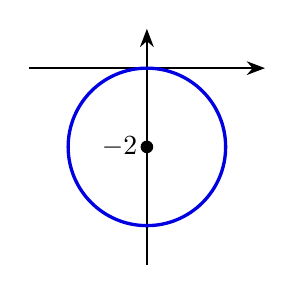
\begin{tikzpicture}
			\draw[cstaxis] (-1.5,0)--(1.5,0);
			\draw[cstaxis] (0,-2.5)--(0,.5);
			\coordinate (A) at (0,-1);
			\fill[cstdot] (A) circle
				node[left] {$-2\ii $};
			\draw[cstcurve,main] (A) circle (1);
		\end{tikzpicture}}
	\end{example}
\end{frame}


\begin{frame}{例题: 复数方程表直线}
	\onslide<+->
	\begin{example}[sidepic,righthand width=3.3cm]
		$\abs{z-4\ii}=\abs{z-2}$.
		\onslide<+->{%
			该方程表示与 $4\ii$ 和 $2$ 的距离相等的点, 即二者连线的垂直平分线.
		}\onslide<+->{%
			两边同时平方化简可得 $x-2y+3=0$.
		}\onslide<+->{%
			该方程也可以表达为
			\[
				(1+2\ii)z+(1-2\ii)\ov z+6=0.
			\]
		}
		\tcblower
		\onslide<2->{
      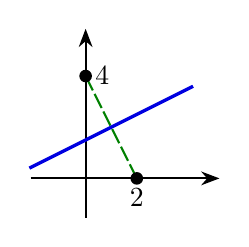
\begin{tikzpicture}[
        declare function={
          f(\y)=2*\y-1.5;
        }
      ]
        \def\u{.65}
        \draw[cstaxis] (-.7,0)--(1.7,0);
        \draw[cstaxis] (0,-.5)--(0,1.9);
        \coordinate (A) at (\u,0);
        \coordinate (B) at (0,{2*\u});
        \draw[cstdash,fourth] (A)--(B);
        \draw[cstcurve,main] ({f(.2)*\u},{.2*\u})--({f(1.8)*\u},{1.8*\u});
        \begin{scope}[cstdot]
          \fill (A) circle node[below] {$2$};
          \fill (B) circle node[right] {$4\ii$};
        \end{scope}
      \end{tikzpicture}}
	\end{example}
\end{frame}


\begin{frame}{例题: 复数方程表椭圆和双曲线}
	\onslide<+->
	\begin{example}
		$\abs{z-z_1}+\abs{z-z_2}=2a$.
		\begin{itemize}
			\item 当 $2a>\abs{z_1-z_2}$ 时, 该方程表示以 $z_1,z_2$ 为焦点, $a$ 为长半轴的椭圆;
			\item 当 $2a=\abs{z_1-z_2}$ 时, 该方程表示连接 $z_1,z_2$ 的线段;
			\item 当 $2a<\abs{z_1-z_2}$ 时, 该方程表示空集.
		\end{itemize}
	\end{example}
	\onslide<+->
	\begin{example}
		$\abs{z-z_1}-\abs{z-z_2}=2a$.
		\begin{itemize}
			\item 当 $2a<\abs{z_1-z_2}$ 时, 该方程表示以 $z_1,z_2$ 为焦点, $a$ 为实半轴的双曲线的一支;
			\item 当 $2a=\abs{z_1-z_2}$ 时, 该方程表示以 $z_2$ 为起点, 与 $z_2,z_1$ 连线反向的射线;
			\item 当 $2a>\abs{z_1-z_2}$ 时, 该方程表示空集.	
		\end{itemize}
	\end{example}
\end{frame}


\begin{frame}{例题: 复数方程表平面图形}
	\onslide<+->
	\begin{exercise}[nearnext]
		$z^2+\ov z^2=1$ 和 $z^2-\ov z^2=\ii$ 分别表示什么图形?
	\end{exercise}

	\onslide<+->
	\begin{answer}[nearprev]
		双曲线 $x^2-y^2=\dfrac12$ 和双曲线 $xy=\dfrac14$.
	\end{answer}
\end{frame}


\begin{frame}{连续曲线、闭路}
	\onslide<+->
	设 $x(t),y(t),t\in[a,b]$ 是两个连续函数.
	\onslide<+->
	参变量方程 $\begin{cases}
		x=x(t),& \\y=y(t),&
	\end{cases}t\in[a,b]$ 定义了一条\emph{连续曲线}.
	\onslide<+->
	这也等价于 $C:z=z(t)=x(t)+\ii y(t),t\in[a,b]$.
	\begin{itemize}
		\item 若除了两个端点有可能重叠外, 其它情形不会出现重叠的点, 则称 $C$ 是\emph{简单曲线}.
		\item 若连续曲线 $C$ 满足两个端点重叠, 即 $z(a) = z(b)$, 则称 $C$ 是闭合曲线.
		\item 称闭合的简单曲线为\emph{简单闭曲线}或\emph{闭路}.
	\end{itemize}
	\onslide<3->
	\begin{center}
		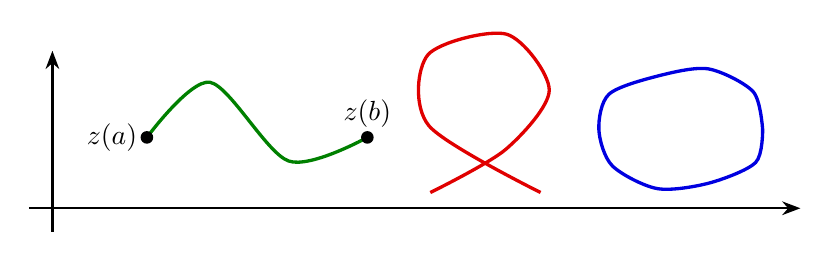
\begin{tikzpicture}
			\draw[cstaxis](-.3,.5)--(9.5,.5);
			\draw[cstaxis](0,.2)--(0,2.5);
			\coordinate (A) at (1.2,1.4);
			\coordinate (B) at (4,1.4);
			\draw[cstcurve,fourth,smooth] plot coordinates {(A) (2,2.1) (3,1.1) (B)};
			\fill[cstdot] (A) circle node[left] {$z(a)$};
			\fill[cstdot] (B) circle node[above] {$z(b)$};
			\draw[cstcurve,second,smooth,visible on=<4->] plot coordinates {(4.8,.7) (5.76,1.25) (6.31,2) (5.77,2.71) (4.77,2.45) (4.78,1.55) (6.2,.7) };
			\draw[cstcurve,main,smooth,visible on=<5->] plot coordinates {(9.02,1.5) (8.9,1.98) (8.33,2.27) (7.69,2.18) (7.07,1.95) (6.94,1.5) (7.11,1.04) (7.68,.75) (8.34,.82) (8.93,1.08) (9.02,1.5)};
		\end{tikzpicture}
	\end{center}
\end{frame}


\begin{frame}{例题: 连续曲线}
	\onslide<+->
	\begin{example}[near]
		圆 $\abs{z-z_0}=R$ 的参数方程: $z=z_0+R\ee^{\ii\theta},\quad\theta\in[0,2\pi]$.
	\end{example}
	\onslide<+->
	\begin{example}[sidepic,righthand width=150pt,near]
		直线段:
		\[
			z(t)=z_0+(z_1-z_0)t,\quad t\in[0,1],
		\]
		其中 $z_0,z_1$ 为两个端点.
		它是简单曲线.
		\tcblower
		\begin{center}
			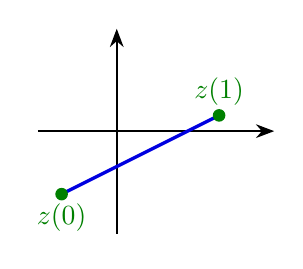
\begin{tikzpicture}
				\draw[cstaxis] (-1.3,.3)--(1.7,.3);
				\draw[cstaxis] (-.3,-1)--(-.3,1.6);
				\coordinate (A) at (-1,-.5);
				\coordinate (B) at (1,.5);
				\draw[cstcurve,main] (A)--(B);
				\begin{scope}[cstdot,fourth]
					\fill (A) circle node[below] {$z(0)$};
					\fill (B) circle node[above] {$z(1)$};
				\end{scope}
			\end{tikzpicture}
		\end{center}
	\end{example}
	\onslide<+->
	\begin{example}[sidepic,righthand width=150pt,near]
		正弦函数曲线段
		\[
			z(t)=\sin t,\quad t\in[0,2\pi]
		\]
		是简单曲线.
		\tcblower
		\begin{center}
			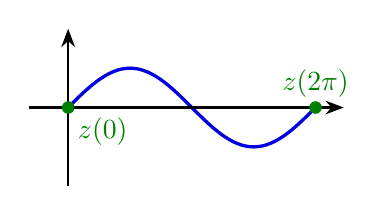
\begin{tikzpicture}
				\draw[cstcurve,main,domain=0:360,smooth] plot ({\x*pi/360},{sin(\x)*.5});
				\draw[cstaxis] (0,-1)--(0,1);
				\draw[cstaxis] (-.5,0)--(3.5,0);
				\coordinate (C) at (0,0);
				\coordinate (D) at ({pi},0);
				\begin{scope}[cstdot,fourth]
					\fill (C) circle node[below right] {$z(0)$};
					\fill (D) circle node[above] {$z(2\pi)$};
				\end{scope}
			\end{tikzpicture}
		\end{center}
	\end{example}
\end{frame}


\begin{frame}{例题: 连续曲线}
	\onslide<+->
	\begin{example}[sidepic,righthand width=150pt]
		椭圆 $\abs{z-\sqrt5}+\abs{z+\sqrt5}=6$ 的参数方程: 
		\[
			z=3\cos\theta+2\ii\sin\theta,\quad \theta\in[0,2\pi].
		\]
		\tcblower
		\begin{center}
			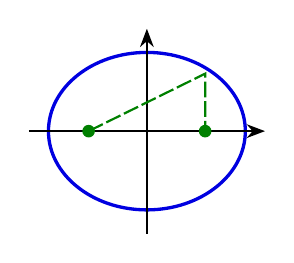
\begin{tikzpicture}
				\coordinate (E) at (-.74,0);
				\coordinate (F) at (.74,0);
				\draw[cstcurve,main] (0,0) circle(1.25 and 1);
				\draw[cstaxis] (-1.5,0)--(1.5,0);
				\draw[cstaxis] (0,-1.3)--(0,1.3);
				\draw[cstdash,fourth] (E)--(.74,.73)--(F);
				\begin{scope}[cstdot,fourth]
					\fill (E) circle;
					\fill (F) circle;
				\end{scope}
			\end{tikzpicture}
		\end{center}
	\end{example}
	\onslide<+->
	\begin{example}[sidepic,righthand width=150pt]
		双纽线 $\abs{z^2-1}=1$ 是闭合曲线, 但不是闭路.
		\tcblower
		\begin{center}
			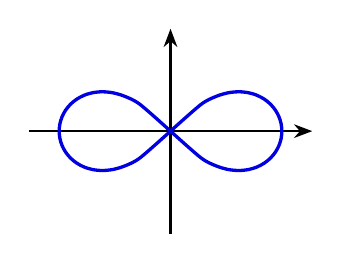
\begin{tikzpicture}
				\draw[cstaxis] (-1.8,0)--(1.8,0);
				\draw[cstaxis] (0,-1.3)--(0,1.3);
				\draw[cstcurve,main,domain=-45:45,smooth] plot ({sqrt(2*cos(2*\x))*cos(\x)},{sqrt(2*cos(2*\x))*sin(\x)});
				\draw[cstcurve,main,domain=-45:45,smooth] plot ({-sqrt(2*cos(2*\x))*cos(\x)},{sqrt(2*cos(2*\x))*sin(\x)});
			\end{tikzpicture}
		\end{center}
	\end{example}
\end{frame}


\subsection{区域和闭区域}


\begin{frame}{邻域}
	\onslide<+->
	为了引入极限的概念, 我们需要考虑点的邻域.
	\onslide<+->
	类比于高等数学中的邻域和去心邻域, 我们在复变函数中, 称开圆盘
		\[
			U(z_0,\delta)=\{z:\abs{z-z_0}<\delta\}
		\]
		为 $z_0$ 的一个 \emph{$\delta$-邻域}.
	\onslide<+->
	称去心开圆盘
		\[
			\Uc(z_0,\delta)=\{z:0<\abs{z-z_0}<\delta\}
		\]
		为 $z_0$ 的一个\emph{去心 $\delta$-邻域}.
	\onslide<2->
	\begin{center}
		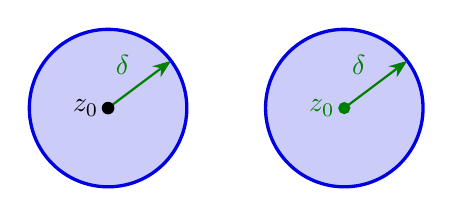
\begin{tikzpicture}
			\begin{scope}
				\coordinate (A) at (-1,0);
				\coordinate (B) at (2,0);
				\filldraw[cstcurve,main,cstfill1] (A) circle (1);
				\filldraw[cstcurve,main,cstfill1,visible on=<3->] (B) circle (1);
				\draw[cstra,fourth,thick] (A)--++(.8,.6)
					node[midway,above left] {$\delta$};
				\draw[cstra,fourth,thick,visible on=<3->] (B)--++(.8,.6)
					node[midway,above left] {$\delta$};
			\end{scope}
			\fill[cstdot] (A) circle node[left] {$z_0$};
			\filldraw[cstdote,fourth,visible on=<3->] (B) circle node[left] {$z_0$};
		\end{tikzpicture}
	\end{center}
\end{frame}


\begin{frame}{内部、外部、边界}
	\onslide<+->
	设 $G$ 是复平面的一个子集, $z_0\in\BC$.
	\onslide<+->
	它们的位置关系有三种可能:
		\begin{enumerate}
			\item 若存在 $z_0$ 的一个邻域 $U$ 完全包含在 $G$ 中, 则称 $z_0$ 是 $G$ 的一个\emph{内点}.
			\item 若存在 $z_0$ 的一个邻域 $U$ 完全不包含在 $G$ 中, 则称 $z_0$ 是 $G$ 的一个\emph{外点}.
			\item 若 $z_0$ 既不是内点也不是外点, 则称 $z_0$ 是 $G$ 的一个\emph{边界点}.
		\end{enumerate}
	\onslide<+->
	内点都属于 $G$, 外点都不属于 $G$, 而边界点则都有可能.
	\onslide<+->
	这类比于区间的端点和区间的关系.
	\onslide<1->
	\begin{center}
		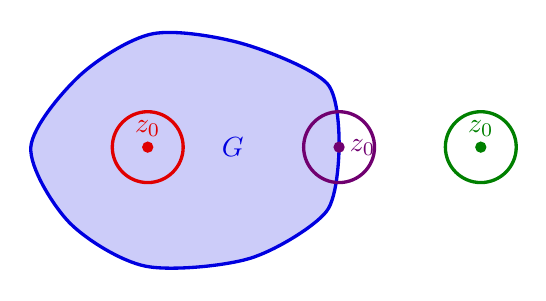
\begin{tikzpicture}[scale=.9]
			\filldraw[cstcurve,main,cstfill1,smooth] plot coordinates {(2,0) (1.83,.9) (.64,1.46) (-.63,1.6) (-1.66,1.01) (-2.35,0) (-1.81,-1.06) (-.73,-1.68) (.74,-1.57) (1.82,-.91) (2,0)};
			\begin{scope}[visible on=<3->]
				\coordinate (A) at (-.7,0);
				\draw[cstcurve,second] (A) circle (.5) node[above] {$z_0$};
				\fill[cstdot,second] (A) circle;
			\end{scope}
			\begin{scope}[visible on=<5->]
				\coordinate (B) at (2,0);
				\draw[cstcurve,third] (B) circle (.5) node[right] {$z_0$};
				\fill[cstdot,third] (B) circle;
			\end{scope}
			\begin{scope}[visible on=<4->]
				\coordinate (C) at (4,0);
				\draw[cstcurve,fourth] (C) circle (.5) node[above] {$z_0$};
				\fill[cstdot,fourth] (C) circle;
			\end{scope}
			\draw (.5,0) node[main] {$G$};
		\end{tikzpicture}
	\end{center}
\end{frame}


\begin{frame}{开集和闭集、有界和无界}
	\onslide<+->
	\begin{definition}[nearnext]
		\begin{enumerate}
			\item 若 $G$ 的所有点都是内点, 也就是说, $G$ 的边界点都不属于它, 称 $G$ 是一个\emph{开集}.
			\item 若 $G$ 的所有边界点都属于 $G$, 称 $G$ 是一个\emph{闭集}.
		\end{enumerate}
	\end{definition}
	\onslide<+->
	$G$ 是一个闭集当且仅当它的补集是开集.

	\onslide<+->
	例如
	\[
		\abs{z-z_0}<R,\quad 1<\Re z<3,\quad\frac\pi4<\arg z<\dfrac{3\pi}4
	\]
	都是开集.
	\onslide<+->
	直观上看: 开集往往由 $>,<$ 的不等式给出, 闭集往往由 $\ge,\le$ 的不等式给出. 
	\onslide<+->
	不过注意这并不是绝对的.

	\onslide<+->
	若 $D$ 可以被包含在某个开圆盘 $U(0,R)$ 中, 则称它是\emph{有界}的.
	\onslide<+->
	否则称它是\emph{无界}的.
\end{frame}


\begin{frame}{区域和闭区域}
	\onslide<+->
	\begin{definition}
		若开集 $D$ 的任意两个点之间都可以用一条完全包含在 $D$ 中的折线连接起来, 则称 $D$ 是一个\emph{区域}.
		\onslide<+->{%
			也就是说, 区域是连通的开集.
		}
	\end{definition}
	\onslide<+->
	\begin{twopart}[indent]{132pt}
		观察右侧图案, 阴影部分(不包含线条部分)中任意两点可用折线连接, 因此它是一个区域.
		\onslide<+->
		这些线条和点构成了它的边界.

		\onslide<+->
		区域和它的边界一起构成了\emph{闭区域}, 记作 $\ov D$.
		\onslide<+->
		它是一个闭集.
		\tcblower
		\onslide<3->
		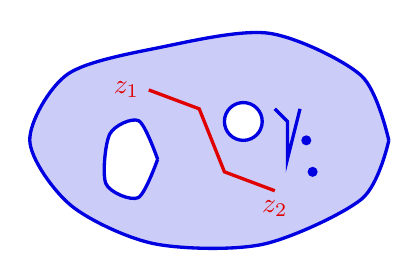
\begin{tikzpicture}[scale=.8]
			\filldraw[cstcurve,main,cstfill1,smooth] plot coordinates {(2.81,0) (2.37,1.03) (.91,1.7) (-.8,1.48) (-2.29,1.05) (-2.89,0) (-2.24,-1.03) (-.92,-1.64) (.81,-1.65) (2.38,-.93) (2.81,0)};
			\filldraw[cstcurve,main,fill=white,smooth] plot coordinates {(-.86,-.3) (-1.16,.31) (-1.62,.1) (-1.68,-.69) (-1.17,-.91) (-.86,-.3)};
			\filldraw[cstcurve,main,fill=white] (.5,.3) circle (.3);
			\fill[cstdot,main] (1.5,0) circle;
			\fill[cstdot,main] (1.6,-.5) circle;
			\draw[cstcurve,second,main] plot coordinates {(1,.5) (1.2,.3) (1.2,-.3) (1.4,.5)};
			\coordinate [label=left:\textcolor{second}{$z_1$}] (A) at (-1,.8);
			\coordinate [label=below:\textcolor{second}{$z_2$}] (B) at (1,-.8);
			\draw[cstcurve,second] (A)--(-.2,.5)--(.2,-.5)--(B);
		\end{tikzpicture}
	\end{twopart}
	\onslide<+->
	注意数学中边界的概念与日常所说的边界是两码事.
	\onslide<+->
	例如区域 $\abs{z}>1$ 的边界是 $\abs{z}=1$, 其闭区域是 $\abs{z}\ge 1$.
\end{frame}


\begin{frame}{常见区域}\small
	\onslide<+->
	很多区域可以由复数的实部、虚部、模和辐角的不等式所确定.
	\onslide<7->{%
		下方区域对应的闭区域是什么?
	}\bigdel
	\onslide<2->
	\begin{figure}[hbpt]
		\begin{minipage}{.24\textwidth}
			\centering
			\begin{tikzpicture}[scale=.7]
				\draw[cstaxis](-1.5,0)--(1.5,0);
				\draw[cstaxis](0,-1.5)--(0,1.5);
				\fill[cstfille1] (-1.2,0) rectangle (1.2,.8);
				\draw (0,-1.5) node[below,align=center] {上半平面\\$\Im z>0$};
			\end{tikzpicture}
		\end{minipage}
		\begin{minipage}{.24\textwidth}
			\centering
			\begin{tikzpicture}[scale=.7]
				\draw[cstaxis](-1.5,0)--(1.5,0);
				\draw[cstaxis](0,-1.5)--(0,1.5);
				\fill[cstfille1] (-1.2,0) rectangle (1.2,-.8);
				\draw (0,-1.5) node[below,align=center] {下半平面\\$\Im z<0$};
			\end{tikzpicture}
		\end{minipage}
		\begin{minipage}{.24\textwidth}
			\centering
			\begin{tikzpicture}[scale=.7,visible on=<3->]
				\draw[cstaxis](-1.5,0)--(1.5,0);
				\draw[cstaxis](0,-1.5)--(0,1.5);
				\fill[cstfille1] (-1.2,-1) rectangle (0,1);
				\draw (0,-1.5) node[below,align=center] {左半平面\\$\Re z<0$};
			\end{tikzpicture}
		\end{minipage}
		\begin{minipage}{.24\textwidth}
			\centering
			\begin{tikzpicture}[scale=.7,visible on=<3->]
				\draw[cstaxis](-1.5,0)--(1.5,0);
				\draw[cstaxis](0,-1.5)--(0,1.5);
				\fill[cstfille1] (0,1) rectangle (1.2,-1);
				\draw (0,-1.5) node[below,align=center] {右半平面\\$\Re z>0$};
			\end{tikzpicture}
		\end{minipage}
	\end{figure}
	\vspace{-.5\baselineskip}	
	\begin{figure}[hbpt]
		\begin{minipage}{.24\textwidth}
			\centering
			\begin{tikzpicture}[scale=.7,visible on=<4->]
				\draw[cstaxis](-1.5,0)--(1.5,0);
				\draw[cstaxis](0,-1.5)--(0,1.5);
				\fill[cstfille1] (-.6,-1) rectangle (.2,1);
				\draw[cstcurve,main] (-.6,-1)--(-.6,1);
				\draw[cstcurve,main] (.2,-1)--(.2,1);
				\draw (0,-1.5) node[below,align=center] {竖直带状区域\\$x_1<\Re z<x_2$};
			\end{tikzpicture}
		\end{minipage}
		\begin{minipage}{.24\textwidth}
			\centering
			\begin{tikzpicture}[scale=.7,visible on=<4->]
				\draw[cstaxis](-1.5,0)--(1.5,0);
				\draw[cstaxis](0,-1.5)--(0,1.5);
				\fill[cstfille1] (-1,-.4) rectangle (1,.4);
				\draw[cstcurve,main] (-1,-.4)--(1,-.4);
				\draw[cstcurve,main] (-1,.4)--(1,.4);
				\draw (0,-1.5) node[below,align=center] {水平带状区域\\$y_1<\Im z<y_2$};
			\end{tikzpicture}
		\end{minipage}
		\begin{minipage}{.24\textwidth}
			\centering
			\begin{tikzpicture}[scale=.7,visible on=<5->]
				\draw[cstaxis](-.5,0)--(2.5,0);
				\draw[cstaxis](0,-.5)--(0,2.5);
				\coordinate (A) at (0,0);
				\coordinate (B) at ({2.2*cos(60)},{2.2*sin(60)});
				\coordinate (C) at ({2.2*cos(10)},{2.2*sin(10)});
				\fill[cstfille1] (A)--(B) arc(60:10:2.2)--cycle;
				\draw[cstcurve,main] (C)--(A)--(B);
				\draw (1,-.5) node[below,align=center] {角状区域\\$\alpha_1<\arg z<\alpha_2$};
			\end{tikzpicture}
		\end{minipage}
		\begin{minipage}{.24\textwidth}
			\centering
			\begin{tikzpicture}[scale=.7,visible on=<6->]
				\filldraw[cstcurve,main,cstfill1] (0,0) circle (1.2);
				\filldraw[cstcurve,main,fill=white] (0,0) circle (.6);
				\draw[cstaxis](-1.5,0)--(1.5,0);
				\draw[cstaxis](0,-1.5)--(0,1.5);
				\draw (0,-1.5) node[below,align=center] {圆环域\\$r<\abs{z}<R$};
			\end{tikzpicture}
		\end{minipage}
	\end{figure}
\end{frame}


\subsection{区域的特性}


\begin{frame}{闭路的内部和外部}
	\onslide<+->
	闭路 $C$ 把复平面划分成了两个区域, 一个有界一个无界.
	\onslide<+->
	分别称这两个区域是 $C$ 的\emph{内部}和\emph{外部}.
	\onslide<+->
	$C$ 是它们的公共边界.
	\onslide<1->
	\begin{center}
		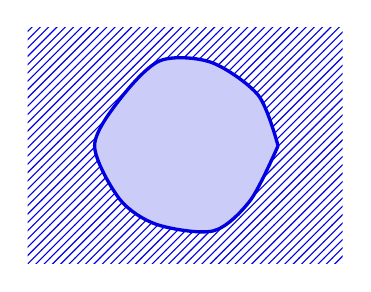
\begin{tikzpicture}
			\fill[cstfille1] (-2,-1.5) rectangle (2,1.5);
			\filldraw[cstcurve,main,cstfill1,smooth] plot coordinates {(1.18,0) (.93,.64) (.33,1.06) (-.32,1.08) (-.83,.59) (-1.15,0) (-.83,-.68) (-.36,-1) (.36,-1.08) (.83,-.69) (1.18,0)};
		\end{tikzpicture}
	\end{center}
\end{frame}


\begin{frame}{单连通区域和多连通区域}
	\onslide<+->
	在前面所说的几个常见区域的例子中, 我们在区域中画一条闭路.
	\onslide<+->
	除了圆环域之外, 闭路的内部仍然包含在这个区域内.
	\onslide<+->
	\begin{definition}
		若区域 $D$ 中的任一闭路的内部都包含在 $D$ 中, 则称 $D$ 是\emph{单连通区域}.
		否则称之为\emph{多连通区域}.
	\end{definition}
	\onslide<+->
	单连通区域内的任一闭路可以``连续地变形''成一个点.
	\onslide<+->
	这也等价于: 设 $\ell_0,\ell_1$ 是从 $A$ 到 $B$ 的两条连续曲线, 则 $\ell_0$ 可以连续地变形为 $\ell_1$ 且保持端点不动.
	\onslide<4->
	\bigdel
	\begin{center}
		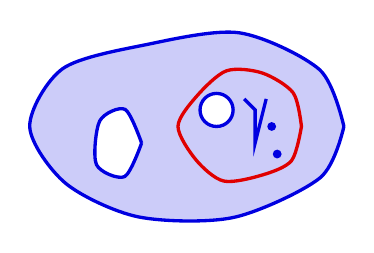
\begin{tikzpicture}[scale=.7]
			\filldraw[cstcurve,main,cstfill1,smooth] plot coordinates {(2.81,0) (2.37,1.03) (.91,1.7) (-.8,1.48) (-2.29,1.05) (-2.89,0) (-2.24,-1.03) (-.92,-1.64) (.81,-1.65) (2.38,-.93) (2.81,0)};
			\filldraw[cstcurve,main,fill=white,smooth] plot coordinates {(-.86,-.3) (-1.16,.31) (-1.62,.1) (-1.68,-.69) (-1.17,-.91) (-.86,-.3)};
			\filldraw[cstcurve,main,fill=white] (.5,.3) circle (.3);
			\fill[cstdot,main] (1.5,0) circle;
			\fill[cstdot,main] (1.6,-.5) circle;
			\draw[cstcurve,main] plot coordinates {(1,.5) (1.2,.3) (1.2,-.3) (1.4,.5)};
			\draw[cstcurve,second,smooth,visible on=<5->,shift={(.1,.2)}] plot coordinates {(1.94,-.2) (1.79,.41) (1.23,.77) (.58,.81) (.04,.35) (-.3,-.2) (.03,-.81) (.53,-1.19) (1.23,-1.08) (1.76,-.82) (1.94,-.2)};
		\end{tikzpicture}
	\end{center}
\end{frame}


\begin{frame}{典型例题: 区域的特性}
	\onslide<+->
	\begin{example}[sidepic,righthand width=3.3cm]
		$\Re(z^2)<1$.
		\onslide<+->{%
			设 $z=x+y\ii$, 则 $\Re(z^2)=x^2-y^2<1$.
		}\onslide<+->{%
			这是无界的单连通区域.
		}
		\tcblower
		\onslide<2->{%
		\begin{center}
			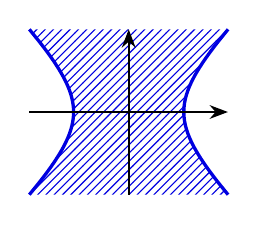
\begin{tikzpicture}[scale=.7]
				\def\t{{atan(1.5)}}
				\fill[cstfille1,domain=-\t:\t,smooth] plot ({sec(\x)},{tan(\x)})
				-- plot[domain=\t:-\t] ({-sec(\x)},{tan(\x)})
				--cycle;
				\draw[cstcurve,main,domain=-\t:\t,smooth] plot ({sec(\x)},{tan(\x)});
				\draw[cstcurve,main,domain=-\t:\t,smooth] plot ({-sec(\x)},{tan(\x)});
				\draw[cstaxis] (-1.8,0)--(1.8,0);
				\draw[cstaxis] (0,-1.5)--(0,1.5);
			\end{tikzpicture}
		\end{center}}
	\end{example}
	\onslide<+->
	\begin{example}[sidepic,righthand width=3.3cm]
		$\arg z\neq \pi$. 
		\onslide<+->{%
			即角状区域 $-\pi<\arg z<\pi$.
		}\onslide<+->{%
			这是无界的单连通区域.
		}
		\tcblower
		\onslide<5->{%
		\begin{center}
			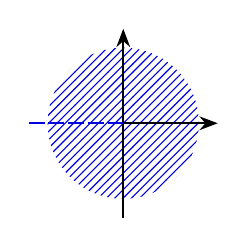
\begin{tikzpicture}[scale=.8]
				\fill[cstfille1] (0,0) circle (1.2);
				\draw[cstaxis] (0,0)--(1.5,0);
				\draw[cstaxis] (0,-1.5)--(0,1.5);
				\draw[cstdash,main] (-1.5,0)--(0,0);
			\end{tikzpicture}
		\end{center}}
	\end{example}
\end{frame}


\begin{frame}{典型例题: 区域的特性}
	\onslide<+->
	\begin{example}[near,sidepic,righthand width=3.3cm]
		$\Bigabs{\dfrac1z}\le3$.
		\onslide<+->{%
			即 $\abs{z}\ge\dfrac13$.
		}\onslide<+->{%
			这是无界的多连通\alertn{闭区域}.
		}
		\tcblower
		\onslide<2->{%
		\begin{center}
			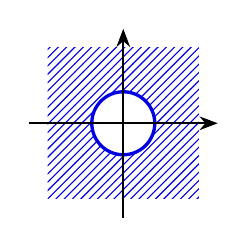
\begin{tikzpicture}[scale=.8]
				\fill[cstfille1] (-1.2,-1.2) rectangle (1.2,1.2);
				\filldraw[cstcurve,main,fill=white] (0,0) circle (.5);
				\draw[cstaxis] (-1.5,0)--(1.5,0);
				\draw[cstaxis] (0,-1.5)--(0,1.5);
			\end{tikzpicture}
		\end{center}}
	\end{example}
	\onslide<+->
	\begin{example}[near,sidepic,righthand width=3.3cm]
		$\abs{z+1}+\abs{z-1}<4$.
		\onslide<+->{%
			表示一个椭圆的内部.
		}\onslide<+->{%
			这是有界的单连通区域.
		}
		
		\tcblower
		\onslide<5->{%
		\begin{center}
			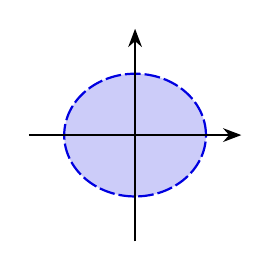
\begin{tikzpicture}[scale=.9]
				\filldraw[cstdash,main,cstfill1] (0,0) circle (1 and {0.5*sqrt(3)});
				\draw[cstaxis] (-1.5,0)--(1.5,0);
				\draw[cstaxis] (0,-1.5)--(0,1.5);
			\end{tikzpicture}
		\end{center}}
	\end{example}
	\onslide<+->
	\begin{exercise}[near]
		$\abs{z+1}+\abs{z-1}\ge 1$ 表示什么集合?
		\onslide<+->{\alertn{整个复平面.}}
	\end{exercise}
\end{frame}


\section{分块矩阵}

\subsection{分块矩阵的定义和运算}

\begin{frame}{分块矩阵的定义}
	\onslide<+->
	有时为了研究矩阵和其部分元素形成的矩阵的联系, 需要使用\emph{分块法}将其进行拆分:
	\onslide<+->
	\begin{definition}[分块矩阵]
		用若干条横线和竖线将矩阵 $\bfA$ 分成许多小矩阵, 每个小矩阵成为 $\bfA$ 的子块, 以子块为元素的矩阵称为\emph{分块矩阵}.
	\end{definition}
	\onslide<+->
	例如
	\[\bfA=\begin{pmatrix}
		\bfO_{m\times n}&\bfE_m\\
		\bfE_n&\bfO_{n\times m}
	\end{pmatrix}\]
	就是一个分块矩阵.
	\onslide<+->
	事实上我们已经不加声明地用过分块矩阵了.
\end{frame}


\begin{frame}{分块矩阵的运算: 加法和数乘}
	\onslide<+->
	若分块矩阵 $\bfA,\bfB$ 同型, 且每个对应分块也同型, 则 $\bfA+\bfB$ 就是对应分块相加形成的分块矩阵:
	\[\begin{pmatrix}
		\bfA_{11}&\cdots&\bfA_{1r}\\
		\vdots&\ddots&\vdots\\
		\bfA_{s1}&\cdots&\bfA_{sr}
	\end{pmatrix}+\begin{pmatrix}
		\bfB_{11}&\cdots&\bfB_{1r}\\
		\vdots&\ddots&\vdots\\
		\bfB_{s1}&\cdots&\bfB_{sr}
	\end{pmatrix}=\begin{pmatrix}
		\bfA_{11}+\bfB_{11}&\cdots&\bfA_{1r}+\bfB_{1r}\\
		\vdots&\ddots&\vdots\\
		\bfA_{s1}+\bfB_{s1}&\cdots&\bfA_{sr}+\bfB_{sr}
	\end{pmatrix}.\]

	\onslide<+->
	数 $\lambda$ 和分块矩阵的数乘, 就是 $\lambda$ 和对应分块数乘形成的分块矩阵:
	\[\lambda\begin{pmatrix}
		\bfA_{11}&\cdots&\bfA_{1r}\\
		\vdots&\ddots&\vdots\\
		\bfA_{s1}&\cdots&\bfA_{sr}
	\end{pmatrix}=\begin{pmatrix}
		\lambda\bfA_{11}&\cdots&\lambda\bfA_{1r}\\
		\vdots&\ddots&\vdots\\
		\lambda\bfA_{s1}&\cdots&\lambda\bfA_{sr}
	\end{pmatrix}.\]
\end{frame}


\begin{frame}{分块矩阵的运算: 乘法}
	\onslide<+->
	设
	\[\bfA=\begin{pmatrix}
		\bfA_{11}&\cdots&\bfA_{1r}\\
		\vdots&\ddots&\vdots\\
		\bfA_{s1}&\cdots&\bfA_{sr}
	\end{pmatrix},\quad
	\bfB=\begin{pmatrix}
		\bfB_{11}&\cdots&\bfB_{1t}\\
		\vdots&\ddots&\vdots\\
		\bfB_{r1}&\cdots&\bfB_{rt},
	\end{pmatrix}\]
	且 $\bfA_{ij}$ 的列数和 $\bfB_{jk}$ 的行数相同, 则
	\[\bfA\bfB=\begin{pmatrix}
		\bfC_{11}&\cdots&\bfC_{1r}\\
		\vdots&\ddots&\vdots\\
		\bfC_{s1}&\cdots&\bfC_{sr}
	\end{pmatrix},\quad\bfC_{ij}=\sum_{k=1}^r \bfA_{ik}\bfB_{kj}.\]
	\onslide<+->
	简单来说就是, 若对应的分块能做相应运算, 则分块矩阵的运算就如同把这些分块视作数一样运算.
\end{frame}


\begin{frame}{分块矩阵的运算: 转置}
	\onslide<+->
	设
	\[\bfA=\begin{pmatrix}
		\bfA_{11}&\cdots&\bfA_{1r}\\
		\vdots&\ddots&\vdots\\
		\bfA_{s1}&\cdots&\bfA_{sr}
	\end{pmatrix},\]
	则
	\[\bfA^\rmT=\begin{pmatrix}
		\bfA_{11}^\rmT&\cdots&\bfA_{s1}^\rmT\\
		\vdots&\ddots&\vdots\\
		\bfA_{1r}^\rmT&\cdots&\bfA_{sr}^\rmT
	\end{pmatrix}.\]
	\onslide<+->
	注意小块的位置需要转置, 每个小块也需要转置.
\end{frame}


\subsection{特殊分块矩阵}
\begin{frame}{分块对角阵}
	\onslide<+->
	若方阵
	\[\bfA=\begin{pmatrix}
		\bfA_1&&\\
		&\ddots&\\
		&&\bfA_m
	\end{pmatrix},\]
	其中 $\bfA_1,\dots,\bfA_m$ 都是方阵,
	\onslide<+->
	称 $\bfA$ 为\emph{分块对角阵}.
	\onslide<+->
	记作 $\bfA=\diag(\bfA_1,\dots,\bfA_m)$.

	\onslide<+->
	分块对角阵具有如下性质:
	\begin{enumerate}
		\item $|\bfA|=|\bfA_1|\cdots|\bfA_m|$;
		\item $\bfA$ 可逆当且仅当 $\bfA_1,\dots,\bfA_m$ 均可逆, 此时
		$\bfA^{-1}=\diag(\bfA_1^{-1},\dots,\bfA_m^{-1})$.
		\item $\bfA^k=\diag(\bfA_1^k,\dots,\bfA_m^k)$.
	\end{enumerate}
\end{frame}


\begin{frame}{例: 分块对角阵}
	\onslide<+->
	\begin{example}
		求 $\bfA=\begin{pmatrix}
			2&1&0&0\\
			1&1&0&0\\
			0&0&2&0\\
			0&0&-1&3
		\end{pmatrix}$ 的逆矩阵.
	\end{example}
	\onslide<+->
	\begin{solution}
		设 $\bfA_1=\begin{pmatrix}
			2&1\\1&1
		\end{pmatrix},\bfA_2=\begin{pmatrix}
			2&0\\-1&3
		\end{pmatrix}$,
		\onslide<+->{%
			则 $\bfA_1^{-1}=\begin{pmatrix}
				1&-1\\-1&2
			\end{pmatrix},\quad\bfA_2^{-1}=\dfrac16\begin{pmatrix}
				3&0\\1&2
			\end{pmatrix}$.
		}

		\onslide<+->{%
			故 $\bfA^{-1}=\diag(\bfA_1^{-1},\bfA_2^{-1})=\begin{pNiceMatrix}
				1&-1&&\\
				-1&2&&\\
				&&1/2&0\\
				&&1/6&1/3
			\end{pNiceMatrix}$.
		}
	\end{solution}
\end{frame}


\begin{frame}{例: 分块三角阵的逆}
\beqskip{2pt}
	\onslide<+->
	\begin{example}
		设 $\bfA,\bfB$ 均可逆, 求 $\begin{pmatrix}
			\bfA&\bfO\\\bfC&\bfB
		\end{pmatrix}$ 的逆矩阵.
	\end{example}
	\onslide<+->
	\begin{solution}
		由 $\begin{vmatrix}
			\bfA&\bfO\\\bfC&\bfB
		\end{vmatrix}=|\bfA|\cdot|\bfB|\neq0$ 可知该方阵可逆.
		\onslide<+->{%
			设 $\begin{pmatrix}
				\bfA&\bfO\\\bfC&\bfB
			\end{pmatrix}\begin{pmatrix}
				\bfA_1&\bfA_2\\\bfA_3&\bfA_4
			\end{pmatrix}=\bfE$.
		}
		
		\onslide<+->{%
			则 $\bfA\bfA_1=\bfE, \bfA\bfA_2=\bfO, \bfC\bfA_2+\bfB\bfA_4=\bfE$.
		}\onslide<+->{%
			于是 $\bfA_1=\bfA^{-1},\bfA_2=\bfO,\bfA_4=\bfB^{-1}$.
		}\onslide<+->{%
			再由 $\bfC\bfA_1+\bfB\bfA_3=\bfO$ 可得
			\[\bfA_3=-\bfB^{-1}\bfC\bfA_1=-\bfB^{-1}\bfC\bfA^{-1}.\]
		}\onslide<+->{%
			故 $\begin{pmatrix}
				\bfA&\bfO\\\bfC&\bfB
			\end{pmatrix}^{-1}=\begin{pmatrix}
				\bfA^{-1}&\bfO\\-\bfB^{-1}\bfC\bfA^{-1}&\bfB^{-1}
			\end{pmatrix}$.
		}
	\end{solution}
	\onslide<+->
	由此可知, (分块)上/下三角阵的逆还是(分块)上/下三角阵.
\endgroup
\end{frame}


\begin{frame}{例: 分块方阵的伴随}
	\onslide<+->
	\begin{exercise}
		设 $\bfA,\bfB$ 为同阶方阵, $\bfC=\begin{pmatrix}
			&\bfA\\\bfB&
		\end{pmatrix}$,
		则 $\bfC^*=$\fillbrace{\visible<+->{D}}.
		\begin{taskschoice}(2)
			() $\begin{pmatrix}&\bfA^*\\\bfB^*&\end{pmatrix}$
			() $\begin{pmatrix}&\bfB^*\\\bfA^*&\end{pmatrix}$
			() $\begin{pmatrix}&|\bfB|\bfA^*\\|\bfA|\bfB^*&\end{pmatrix}$
			() $\begin{pmatrix}&|\bfA|\bfB^*\\|\bfB|\bfA^*&\end{pmatrix}$
		\end{taskschoice}
	\end{exercise}
\end{frame}


\section{极限和连续性}


\subsection{数列的极限}


\begin{frame}{数列的极限}
	\begin{itemize}
		\item 类似于实变函数情形, 我们可以定义复变函数的极限.
		\item 我们先来看数列极限的定义.
	\end{itemize}
	\onslide<+->
	\begin{definition}
		设 $\{z_n\}_{n\ge 1}$ 是一个复数列.
		\onslide<+->{%
		若存在复数 $z$ 满足对任意 $\varepsilon>0$, 存在 $N$ 使得当 $n\ge N$ 时, $\abs{z_n-z}<\varepsilon$, 则称 $z$ 是\emph{数列 $\{z_n\}$ 的极限}, 记作 \emph{$\liml_{n\ra\infty}z_n=z$}.
		}
	\end{definition}
	\begin{itemize}
		\item 此时称\emph{极限存在}或\emph{数列收敛}.
		\item 若不存在这样的 $z$, 则称\emph{极限不存在}或\emph{数列发散}.
		\item 可以看出, $\liml_{n\ra\infty}z_n=z$ 等价于实极限 $\liml_{n\ra\infty}\abs{z_n-z}=0$.
	\end{itemize}
\end{frame}


\begin{frame}{极限的四则运算}
	\begin{itemize}
		\item 由于复数列极限的定义和实数列极限的定义在形式上完全相同,
		\item 因此类似地, 极限的四则运算法则对于复数列也是成立的.
	\end{itemize}
	\onslide<+->
	\begin{theorem}
		设 $\liml_{n\to\infty}z_n=z,\liml_{n\to\infty}w_n=w$, 则
		\begin{enumerate}
			\item $\liml_{n\to\infty}(z_n\pm w_n)=z\pm w$;
			\item $\liml_{n\to\infty} z_nw_n=zw$;
			\item 当 $w\neq 0$ 时, $\liml_{n\to\infty}\dfrac{z_n}{w_n}=\dfrac zw$.
		\end{enumerate}
	\end{theorem}
\end{frame}


\begin{frame}{数列收敛的等价刻画}
	\begin{itemize}
		\item 下述定理保证了我们可以使用实数列的敛散性判定方法来研究复数列的敛散性.
	\end{itemize}
	\onslide<+->
	\begin{theorem}[nearnext]
		设 $z_n=x_n+y_n\ii,z=x+y\ii$, 则
		\[
			\liml_{n\ra\infty}z_n=z\iff
			\liml_{n\ra\infty}x_n=x\ \text{且}\ 
			\liml_{n\ra\infty}y_n=y.
		\]
	\end{theorem}
	\onslide<+->
	\begin{proof}[leftupper=0mm,nearprev]
		\begin{itemize}
			\item 我们只需证明 $
			\liml_{n\ra\infty}\abs{z_n-z}=0\iff
			\liml_{n\ra\infty}\abs{x_n-x}=\liml_{n\ra\infty}\abs{y_n-y}=0$.
			\item ``$\Rightarrow$'': 由三角不等式 $0\le \abs{x_n-x}, \abs{y_n-y}\le\abs{z_n-z}$ 和夹逼准则可得知.
			\item ``$\Leftarrow$'': 由极限的四则运算法则可知 $\liml_{n\ra\infty}\bigl(\abs{x_n-x}+\abs{y_n-y}\bigr)=0$.
			\item 再由三角不等式 $0\le\abs{z_n-z}\le\abs{x_n-x}+\abs{y_n-y}$ 和夹逼准则可得.\qedhere
		\end{itemize}
	\end{proof}
\end{frame}


\begin{frame}{例: 数列的敛散性}
	\onslide<+->
	\begin{example}[nearnext]
		设 $z_n=\Bigl(1-\dfrac1n\Bigr)\ee^{\frac{\pi\ii}n}$. 数列 $\{z_n\}$ 是否收敛?
	\end{example}
	\onslide<+->
	\begin{solution}[nearprev,leftupper=0mm]
		\begin{itemize}
			\item 由于
			\[
				x_n=\Bigl(1-\frac1n\Bigr)\cos\frac\pi n\to 1,\quad
				y_n=\Bigl(1-\frac1n\Bigr)\sin\frac\pi n\to 0.
			\]
			\item 因此 $\{z_n\}$ 收敛且 $\liml_{n\to\infty}z_n=1$.
		\end{itemize}
	\end{solution}
\end{frame}


\subsection{无穷远点和复球面}


\begin{frame}{数列极限的等价定义\noexer}
	\begin{itemize}
		\item 数列极限的定义可以用邻域的语言重新表述为:
	\end{itemize}
	\onslide<+->
	\begin{definition}
		$\liml_{n\ra\infty}z_n=z$ 是指: 对 $z$ 的任意 $\delta$ 邻域 $U$, 存在 $N$ 使得当 $n\ge N$ 时, $z_n\in U$.
	\end{definition}
	\begin{itemize}
		\item 若 $\liml_{n\ra\infty}\abs{z_n}=+\infty$, 我们将其记为 \emph{$\liml_{n\ra\infty}z_n=\infty$}.
		\item 这也等价于: 对任意 $X>0$, 存在 $N$ 使得当 $n\ge N$ 时, $\abs{z_n}>X$.
		\item 我们能不能也用邻域的语言来描述 $\liml_{n\ra\infty}z_n=\infty$ 呢?
		\item 我们将介绍复球面的概念, 它是复数的一种几何表示方式且自然地包含无穷远点 $\infty$.
		\item 这种思想是在黎曼研究多值复变函数时引入的.
	\end{itemize}
\end{frame}


\begin{frame}[b]{复球面\noexer}
	\begin{itemize}
		\item 取一个球心在 $z=0$ 的单位球面.
		\item 过 $O$ 做垂直于复平面的直线, 并与球面相交于其中一点 $N$, 称之为北极.
		\item 对于平面上的任意一点 $z$, 连接北极 $N$ 和 $z$ 的直线一定与球面相交于除 $N$ 以外的唯一一个点 $Z$.
		\item 反之, 球面上除了北极外的任意一点 $Z$, 直线 $NZ$ 一定与复平面相交于唯一一点.
		\item 这样, 球面上除北极外的所有点和全体复数建立了一一对应.
	\end{itemize}
	\onslide<1->
	\begin{center}
		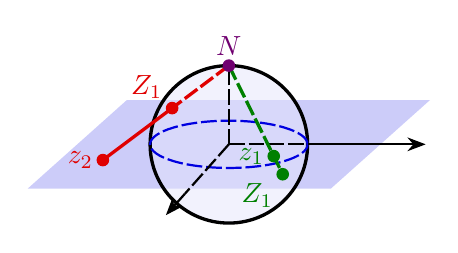
\begin{tikzpicture}
			\begin{scope}[scale=1]
				\fill[cstfill1,scale=.7] (-3.65,-.804)--(-1.85,.804)--(3.65,.804)--(1.85,-.804)--cycle;
				\filldraw[cstcurve,fill=main!10,fill opacity=.5] (0,0) circle (1);
				\draw[cstdash,main] (0,0) circle (1 and 0.3);
				\coordinate [visible on=<2->] (N) at (0,1);
				\draw[cstdash,visible on=<2->] (0,0)--(N);
				\draw[cstdash] (0,0)--(1,0);
				\draw[cstaxis] (1,0)--(2.5,0);
				\def\a{.7}
				\draw[cstdash] (0,0)--({-.8*\a},{-.9*\a});
				\draw[cstaxis] ({-.8*\a},{-.9*\a})--(-.8,-.9);
				\coordinate [visible on=<3->] (z1) at (.57,-.15);
				\coordinate [visible on=<3->] (Z1) at ($(N)!1.2!(z1)$);
				\coordinate [visible on=<4->] (z2) at (-1.6,-.2);
				\coordinate [visible on=<4->] (Z2) at ($(N)!.45!(z2)$);
				\draw[cstdash,cstcurve,fourth,visible on=<3->] (N)--(Z1);
				\draw[cstdash,cstcurve,second,visible on=<4->] (N)--(Z2);
				\draw[cstcurve,second,visible on=<4->] (Z2)--(z2);
			\end{scope}
			\fill[cstdot,fourth,visible on=<3->] (Z1) circle;
			\fill[cstdot,second,visible on=<4->] (Z2) circle;
			\fill[cstdot,fourth,visible on=<3->] (z1) circle;
			\fill[cstdot,second,visible on=<4->] (z2) circle;
			\fill[cstdot,third,visible on=<2->] (N) circle;
			\draw (N) node[third,above,visible on=<2->] {$N$};
			\draw (z1) node[fourth,left,visible on=<3->] {$z_1$};
			\draw (Z1) node[fourth,below left,visible on=<3->] {$Z_1$};
			\draw (z2) node[second,left,visible on=<4->] {$z_2$};
			\draw (Z2) node[second,above left,visible on=<4->] {$Z_1$};
		\end{tikzpicture}
	\end{center}
\end{frame}


\begin{frame}[b]{复球面: 无穷远点\noexer}
	\begin{itemize}
		\item 当 $|z|$ 越来越大时, 其对应球面上点也越来越接近 $N$.
		\item 如果我们在复平面上添加一个额外的"点"——\emph{无穷远点}, 记作 \emph{$\infty$}.
		\item 那么\emph{扩充复数集合 $\BC^*=\BC\cup\{\infty\}$} 就正好和球面上的点一一对应.
		\item 称这样的球面为\emph{复球面}, 称包含无穷远点的复平面为\emph{扩充复平面}或\emph{闭复平面}.
	\end{itemize}
	\onslide<1->
	\begin{center}
		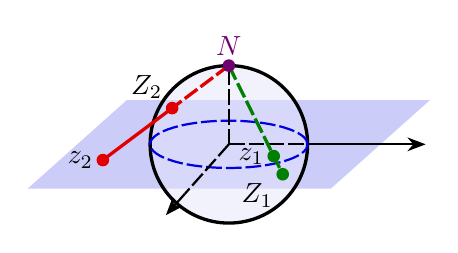
\begin{tikzpicture}
			\begin{scope}[scale=1]
				\fill[cstfill1,scale=.7] (-3.65,-.804)--(-1.85,.804)--(3.65,.804)--(1.85,-.804)--cycle;
				\filldraw[cstcurve,fill=main!10,fill opacity=.5] (0,0) circle (1);
				\draw[cstdash,main] (0,0) circle (1 and 0.3);
				\coordinate [label=above:\textcolor{third}{$N$}] (N) at (0,1);
				\draw[cstdash] (0,0)--(N);
				\draw[cstdash] (0,0)--(1,0);
				\draw[cstaxis] (1,0)--(2.5,0);
				\def\a{.7}
				\draw[cstdash] (0,0)--({-.8*\a},{-.9*\a});
				\draw[cstaxis] ({-.8*\a},{-.9*\a})--(-.8,-.9);
				\coordinate [label=left:{$z_1$}] (z1) at (.57,-.15);
				\coordinate [label=below left:{$Z_1$}] (Z1) at ($(N)!1.2!(z1)$);
				\coordinate [label=left:{$z_2$}] (z2) at (-1.6,-.2);
				\coordinate [label=above left:{$Z_2$}] (Z2) at ($(N)!.45!(z2)$);
				\draw[cstdash,cstcurve,fourth] (N)--(Z1);
				\draw[cstdash,cstcurve,second] (N)--(Z2);
				\draw[cstcurve,second] (Z2)--(z2);
			\end{scope}
			\fill[cstdot,fourth] (Z1) circle;
			\fill[cstdot,second] (Z2) circle;
			\fill[cstdot,fourth] (z1) circle;
			\fill[cstdot,second] (z2) circle;
			\fill[cstdot,third] (N) circle;
		\end{tikzpicture}
	\end{center}
\end{frame}


\begin{frame}{复球面: 无穷远点的邻域\noexer}
	\begin{itemize}
		\item 若约定 $\abs{\infty}=+\infty$, 则分别称
		\[
			U(\infty,X)=\{z\in\BC^*\midcolon \abs{z}>X\},\quad
			\Uc(\infty,X)=\{z\in\BC\midcolon \abs{z}>X\}
		\]
		为 $\infty$ 的 \emph{$X$ 邻域}和\emph{去心 $X$ 邻域}.
		\item 这样, 前述极限可统一表述为: 若对 $z\in\BC^*$ 的任意 $\delta$ 邻域 $U$, 存在 $N$ 使得当 $n\ge N$ 时, $z_n\in U$, 则记 $\liml_{n\ra\infty}z_n=z$.
		\item 朴素地看, 复球面上任意一点可以定义 $\delta$ 邻域为与其距离小于 $\delta$ 的所有点.
		\item 特别地, $\infty$ 的邻域通过前面所说的对应关系, 可以对应到扩充复平面上 $\infty$ 的一个邻域.
		\item 所以在复球面上, 普通复数和 $\infty$ 的邻域具有同等地位.
	\end{itemize}
\end{frame}


\begin{frame}{复球面: 与实数无穷的联系\noexer}
	\begin{itemize}
		\item 它和实数列极限符号中的 $\infty$ 有什么联系呢?
		\item 选取上述图形的一个截面来看, 实轴可以和圆周去掉一点建立一一对应.
		\item 于是实数列极限符号中的 $\infty$ 在复球面上就是 $\infty$.
	\end{itemize}
	\onslide<2->
	\begin{center}
		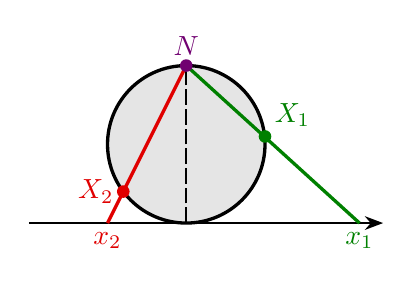
\begin{tikzpicture}
			\filldraw[cstcurve,cstfill] (0,1) circle (1);
			\coordinate [label=above:\textcolor{third}{$N$}] (N) at (0,2);
			\draw[cstdash] (0,0)--(N);
			\draw[cstaxis] (-2,0)--(2.5,0);
			\coordinate [label=below:\textcolor{fourth}{$x_1$}] (x1) at (2.2,0);
			\coordinate [label=above right:\textcolor{fourth}{$X_1$}] (X1) at (1,1.1);
			\coordinate [label=below:\textcolor{second}{$x_2$}] (x2) at (-1,0);
			\coordinate [label=left:\textcolor{second}{$X_2$}] (X2) at (-.8,.4);
			\draw[cstcurve,fourth] (0,2)--(x1);
			\fill[cstdot,fourth] (X1) circle;
			\draw[cstcurve,second] (0,2)--(x2);
			\fill[cstdot,second] (X2) circle;
			\fill[cstdot,third] (N) circle;
		\end{tikzpicture}
	\end{center}
\end{frame}


\subsection{函数的极限}


\begin{frame}{函数的极限}
	\onslide<+->
	\begin{definition}
		设函数 $f(z)$ 在点 $z_0$ 的某个去心邻域内有定义.
		\onslide<+->{%
			如果存在复数 $A$, 使得对 $A$ 的任意邻域 $U(A,\varepsilon),\exists\delta>0$ 使得
			\[z\in\Uc(z_0,\delta)\implies f(z)\in U(A,\varepsilon),
	\]
		}\onslide<+->{%
			则称 $A$ 为 \emph{$f(z)$ 当 $z\to z_0$ 时的极限}, 记为 \emph{$\liml_{z\to z_0}f(z)=A$} 或 \emph{$f(z)\to A (z\to z_0)$}.
		}
	\end{definition}
	\begin{itemize}
		\item 在此表述下, 将上述定义中的 $z_0$ 或 $A$ 换成 $\infty$, 即可得到 $z\ra\infty$ 时的极限定义, 以及 $\lim f(z)=\infty$ 的含义.
	\end{itemize}
\end{frame}


\begin{frame}{极限的四则运算}
	\begin{itemize}
		\item 类似于复数列情形, 极限的四则运算法则对于复变函数也是成立的.
	\end{itemize}
	\onslide<+->
	\begin{theorem}
		设 $\liml_{z\to z_0}f(z)=A,\liml_{z\to z_0}g(z)=B$, 则
		\begin{enumerate}
			\item $\liml_{z\to z_0}(f\pm g)(z)=A\pm B$;
			\item $\liml_{z\to z_0}(fg)(z)=AB$;
			\item 当 $B\neq 0$ 时, $\liml_{z\to z_0}\Bigl(\dfrac fg\Bigr)(z)=\dfrac AB$.
		\end{enumerate}
	\end{theorem}
\end{frame}


\begin{frame}{与实函数极限之联系}
	\begin{itemize}
		\item 和数列极限类似, 我们有下述定理:
	\end{itemize}
	\onslide<+->
	\begin{theorem}
		设 $f(z)=u(x,y)+\ii v(x,y),z_0=x_0+y_0\ii,A=u_0+v_0\ii$, 则
		\[
			\lim_{z\to z_0}f(z)=A\iff
			\lim_{\substack{x\to x_0\\y\to y_0}}u(x,y)=u_0,\quad
			\lim_{\substack{x\to x_0\\y\to y_0}}v(x,y)=v_0.
		\]
	\end{theorem}
	\begin{itemize}
		\item 该定理表明: 研究复变函数极限, 只需研究其实部、虚部两个二元实函数的极限.
		\item 在学习了复变函数的导数后, 我们也可以使用等价无穷小替换、洛必达法则等工具来计算极限.
	\end{itemize}
\end{frame}


\begin{frame}{例: 判断函数极限是否存在}
	\onslide<+->
	\begin{example}[nearnext]
		证明: 当 $z\to0$ 时, 函数 $f(z)=\dfrac{\Re z}{|z|}$ 的极限不存在.
	\end{example}
	\onslide<+->
	\begin{proof}[leftupper=0mm,nearprev]
		\begin{itemize}
			\item 令 $z=x+y\ii$, 则 $f(z)=\dfrac x{\sqrt{x^2+y^2}}$.
			\item 因此
			\[
				u(x,y)=\frac x{\sqrt{x^2+y^2}},\quad v(x,y)=0.
			\]
			\item 当 $z$ 在实轴原点两侧分别趋向于 $0$ 时, $u(x,y)\to\pm1$.
			\item 因此 $\liml_{\substack{x\to 0\\y\to0}}u(x,y)$ 不存在, 从而 $\liml_{z\to z_0}f(z)$ 不存在.\qedhere
		\end{itemize}
		\meddel
	\end{proof}
\end{frame}


\subsection{函数的连续性}


\begin{frame}{函数的连续性}
	\onslide<+->
	\begin{definition}[nearprev]
		\begin{enumerate}
			\item 如果 $\liml_{z\to z_0}f(z)=f(z_0)$, 则称 $f(z)$ 在 \emph{$z_0$ 处连续}.
			\item 如果 $f(z)$ 在区域 $D$ 内处处连续, 则称 $f(z)$ 在 \emph{$D$ 内连续}.
		\end{enumerate}
	\end{definition}
	\onslide<+->
	根据前面的极限判定定理可知:
	\onslide<+->
	\begin{theorem}[nearnext]
		\begin{enumerate}
			\item 函数 $f(z)=u(x,y)+\ii v(x,y)$ 在 $z_0=x_0+\ii y_0$ 处连续当且仅当 $u(x,y)$ 和 $v(x,y)$ 在 $(x_0,y_0)$ 处连续.
			\item 在 $z_0$ 处连续的两个函数 $f(z)$, $g(z)$ 之和、差、积、商($g(z_0)\neq 0$) 在 $z_0$ 处仍然连续.
			\item 如果函数 $g(z)$ 在 $z_0$ 处连续, 函数 $f(w)$ 在 $g(z_0)$ 处连续, 则 $f(g(z))$ 在 $z_0$ 处连续.
		\end{enumerate}
	\end{theorem}
\end{frame}


\begin{frame}{连续函数的性质}
	\onslide<+->
	\begin{example}[near]
		\begin{enumerate}
			\item 设 $f(z)=\ln(x^2+y^2)+\ii(x^2-y^2)$.
			\onslide<+->{%
			$u(x,y)=\ln(x^2+y^2)$ 除原点外处处连续, $v(x,y)=x^2-y^2$ 处处连续.
			}\onslide<+->{%
			因此 $f(z)$ 在 $z\neq0$ 处连续.
			}
			\item 显然 $f(z)=z$ 是处处连续的,
			\onslide<+->{%
			故多项式函数
			\[
				P(z)=a_0+a_1z+a_2z^2+\cdots+a_nz^n
			\]
			也处处连续,
			}\onslide<+->{%
			有理函数 $\dfrac{P(z)}{Q(z)}$ 在 $Q(z)$ 的零点以外处处连续.
			}
		\end{enumerate}
	\end{example}
\end{frame}


\begin{frame}{例: 函数连续性的判定}
	\onslide<+->
	\begin{example}[near]
		证明: 如果 $f(z)$ 在 $z_0$ 连续, 则 $\ov{f(z)}$ 在 $z_0$ 也连续.
	\end{example}
	\onslide<+->
	\begin{proof}[near,leftupper=0mm]
		\begin{itemize}
			\item 设 $f(z)=u(x,y)+\ii v(x,y),z_0=x_0+\ii y_0$.
			\item 那么 $u(x,y),v(x,y)$ 在 $(x_0,y_0)$ 连续.
			\item 从而 $-v(x,y)$ 也在 $(x_0,y_0)$ 连续.
			\item 所以 $\ov{f(z)}=u(x,y)-\ii v(x,y)$ 在 $(x_0,y_0)$ 连续.\qedhere
		\end{itemize}
	\end{proof}
	\onslide<+->
	\begin{proof}[near,leftupper=0mm][另证]
		\begin{itemize}
			\item 函数 $g(z)=\ov z=x-\ii y$ 处处连续,
			\item 从而 $g(f(z))=\ov{f(z)}$ 在 $z_0$ 处连续.\qedhere
		\end{itemize}
	\end{proof}
\end{frame}


\begin{frame}{注记}
	\begin{itemize}
		\item 可以看出, 在极限和连续性上, 复变函数和两个二元实函数没有什么差别.
		\item 那么复变函数和多变量微积分的差异究竟是什么导致的呢?
		\item 归根到底就在于 $\BC$ 是一个域, 上面可以做除法.
		\item 这就导致了复变函数有\alert{导数}, 而不是像多变量实函数只有偏导数.
		\item 这种特性使得可导的复变函数具有整洁优美的性质, 我们将在下一章来逐步揭开它的神秘面纱.
	\end{itemize}
\end{frame}



\part{等价和秩}
\section{向量组}

\subsection{向量组的线性表示}

\begin{frame}{引例题: 齐次线性方程组的解}
	\onslide<+->
	我们知道齐次线性方程组是指 $\bfA\bfx={\bf0}$.
	\onslide<+->
	令
	\[V=\{\bfx\mid \bfA\bfx={\bf0}\}\]
	表示该方程的所有解形成的集合.
	\onslide<+->
	显然 ${\bf0}\in V$.
	\onslide<+->
	若 $\bfu,\bfv\in V$, 则 $\bfA\bfu=\bfA\bfv={\bf0}$.
	\onslide<+->
	于是
	\[\bfA(\bfu+\bfv)=\bfA(\lambda \bfv)={\bf0},\quad \forall\lambda\in\BC.\]
	\onslide<+->
	换言之, $V$ 上的加法和数乘的结果还落在 $V$ 中.
	\onslide<+->
	它是 $\BC^n$ 的一个\emph{子空间}.
	
	\onslide<+->
	如何用有限个向量来表示一个子空间中的所有向量呢?
	\onslide<+->
	我们需要线性组合的概念.
\end{frame}


\begin{frame}{向量组}
	\onslide<+->
	一些具有相同维数的向量放在一起形成\emph{向量组}(可以有重复的):
	\onslide<+->
	例如:
	\begin{itemize}
		\item $\bma_1=(1,1,-1)^\rmT, \bma_2=(2,1,2)^\rmT, \bma_3=(3,2,1)^\rmT$;
		\item $\bma_1^\rmT=(1,1,-1), \bma_2^\rmT=(2,1,2), \bma_3^\rmT=(3,2,1)$;
		\item $m\times n$ 矩阵 $\bfA$ 的 $m$ 行可以看成 $m$ 个行向量, 它们构成一个向量组, 叫做 $\bfA$ 的\emph{行向量组};
		\item 类似地, $\bfA$ 的列向量构成它的\emph{列向量组}.
		\item 对于 $n$ 维向量组
		\[\bfe_1=(1,0,\dots,0)^\rmT,\bfe_2=(0,1,\dots,0)^\rmT,\dots,\bfe_n=(0,0,\dots,1)^\rmT,\]
		\onslide<+->{%
			任意 $n$ 维向量 $\bfx=(x_1,\dots,x_n)^\rmT$ 可以表示为这个向量组中向量的数乘之和:
			\[\bfx=x_1\bfe_1+\cdots+x_n\bfe_n.\]
		}
	\end{itemize}
\end{frame}


\begin{frame}{向量组的线性表示}
	\onslide<+->
	\begin{definition}
		设 $\bma_1,\dots,\bma_m,\bmb$ 为 $n$ 维向量.
		若存在数 $\lambda_1,\dots,\lambda_m$ 使得
		\[\bmb=\lambda_1\bma_1+\cdots+\lambda_m\bma_m,\]
		则称 $\bmb$ 可以被向量组 $\{\bma_1,\dots,\bma_m\}$ \emph{线性表示}, 或称 $\bmb$ 是向量组 $\{\bma_1,\dots,\bma_m\}$ 的\emph{线性组合}.
	\end{definition}
	\onslide<+->
	\begin{example}
		\begin{enumerate}
			\item $n$ 维零向量是任一 $n$ 维向量组的线性组合.
			\item 任意 $n$ 维向量是 $\bfe_1,\dots,\bfe_n$ 的线性组合.
		\end{enumerate}
	\end{example}
\end{frame}


\begin{frame}{线性表示的等价刻画}
	\onslide<+->
	向量 $\bmb$ 能被向量组 $\bma_1,\dots,\bma_m$ 线性表示, 即存在 $\lambda_1,\dots,\lambda_m$ 使得
	\[\bmb=\lambda_1\bma_1+\cdots+\lambda_m\bma_m=(\bma_1,\dots,\bma_m)\begin{pmatrix}
		\lambda_1\\\vdots\\\lambda_m
	\end{pmatrix}.\]
	\vspace{-\baselineskip}
	\onslide<+->
	\begin{theorem}
		向量 $\bmb$ 能被向量组 $\bma_1,\dots,\bma_m$ 线性表示, 当且仅当 $\bfA\bfx=\bmb$ 有解, 其中
		\[\bfA=(\bma_1,\dots,\bma_m)\in M_{n\times m}.\]
	\end{theorem}
	\onslide<+->
	记 $V$ 为向量组 $S=\{\bma_1,\dots,\bma_m\}$ 能线性表示的向量全体.
	\onslide<+->
	容易知道
	\[V=\{\bmb\in\BC^n\mid \text{存在 $\bfx$ 使得}\ \bfA\bfx=\bmb\}\]
	是 $\BC^n$ 的子空间, 称为 $S$ \emph{生成的空间}.
	\onslide<+->
	它是包含 $S$ 中所有向量的最小的线性空间.
\end{frame}


\begin{frame}{向量组的等价}
	\begin{definition}
		\begin{enumerate}
			\item 设有两个向量组 $S=\{\bma_1,\dots,\bma_m\}, T=\{\bmb_1,\dots,\bmb_k\}$.
			若 $\bmb_1,\dots,\bmb_k$ 均可以被 $\{\bma_1,\dots,\bma_m\}$ 线性表示, 则称向量组 $T$ 可以被向量组 $S$ 线性表示.
			\item 若向量组 $S$ 和 $T$ 能相互线性表示, 则称 $S,T$ \emph{向量组等价}.
		\end{enumerate}
	\end{definition}
	\onslide<+->
	设 $S,T$ 分别生成空间 $V,W$.
	\onslide<+->
	$T$ 可以被 $S$ 线性表示$\iff$ $W\subseteq V$;
	\onslide<+->
	$S,T$ 向量组等价$\iff W=V$.

	\onslide<+->
	$T$ 能被 $S$ 线性表示, 当且仅当存在 $\bfx_1,\dots,\bfx_k$ 使得
	\[\bfA\bfx_1=\bmb_1,\quad\dots,\quad\bfA\bfx_k=\bmb_k,\]
	其中 $\bfA=(\bma_1,\dots,\bma_m)$.
	\onslide<+->
	即存在矩阵 $\bfX$ 使得 $\bfA\bfX=\bfB$, 其中 $\bfB=(\bmb_1,\dots,\bmb_k)$.

	\onslide<+->
	反过来, 若 $\bfA\bfX=\bfB$, 则 $\bfB$ 的列向量组可以由 $\bfA$ 的列向量组线性表示.
\end{frame}


\begin{frame}{向量组的等价}
	\onslide<+->
	\begin{theorem}
		\begin{enumerate}
			\item $\bfB$ 的列向量组可以由 $\bfA$ 的列向量组线性表示$\iff$存在矩阵 $\bfX$ 使得 $\bfB=\bfA\bfX$.
			\item $\bfA$ 的列向量组和 $\bfB$ 的列向量组作为向量组等价$\iff$存在矩阵 $\bfX,\bfY$ 使得 $\bfB=\bfA\bfX,\bfA=\bfB\bfY$.
		\end{enumerate}
	\end{theorem}
	\onslide<+->
	\begin{proposition}
		向量组的等价满足如下性质:
		\begin{enumerate}
			\item 自反性: $S\sim S$;
			\item 对称性: $S\sim T\implies T\sim S$;
			\item 传递性: $S\sim T,T\sim R\implies S\sim R$.
		\end{enumerate}
	\end{proposition}
\end{frame}


\subsection{线性相关与线性无关}

\begin{frame}{线性相关与线性无关}
	\onslide<+->
	\begin{definition}
		对于 $n$ 维向量组 $\{\bma_1,\dots,\bma_m\}$,
		若存在一组\alert{不全为零}的数 $\lambda_1,\dots,\lambda_m$ 使得
		\[\lambda_1\bma_1+\dots+\lambda_m\bma_m={\bf0},\]
		则称该向量组\emph{线性相关}.
		否则称该向量组\emph{线性无关}.
	\end{definition}
	\onslide<+->
	向量组 $\{\bma_1,\dots,\bma_m\}$ 线性无关当且仅当
	\[\lambda_1\bma_1+\dots+\lambda_m\bma_m={\bf0}\implies
	\lambda_1=\cdots=\lambda_m=0.\]
	\onslide<+->
	即 $(\bma_1,\cdots,\bma_m)\bfx={\bf0}$ 只有零解.
\end{frame}


\begin{frame}{例题: 线性相关与线性无关}
	\begin{example}
		\begin{enumerate}
			\item $\bma_1=(1,2,3)^\rmT,\bma_2=(2,3,4)^\rmT,\bma_3=(0,0,0)^\rmT$ 线性相关.
			实际上\alert{包含零向量的向量组总是线性相关的}.
			\item $\bma_1=(1,2,3)^\rmT,\bma_2=(2,4,6)^\rmT,\bma_3=(3,0,5)^\rmT$ 线性相关.
			\alert{线性相关的向量组添加更多向量还是线性相关的}.
			\item $\bma_1=(1,2,3)^\rmT,\bma_2=(2,3,4)^\rmT,\bma_3=(3,5,7)^\rmT$ 线性相关.
			它们构成的 $3$ 阶矩阵行列式为零.
			\alert{$n$ 维向量组 $\bma_1,\dots,\bma_n$ 线性无关 $\iff |\bma_1,\cdots,\bma_n|\neq 0$}.
			\item $\bfe_1=(1,0,0)^\rmT,\bfe_2=(0,1,0)^\rmT,\bfe_3=(0,0,1)^\rmT$ 线性无关.
			一般地, \alert{$n$ 维单位向量组 $\bfe_1,\dots,\bfe_n$ 线性无关}.
			\item $\bma$ 线性相关 $\iff \bma\neq{\bf0}$.
			\item $\bma_1,\bma_2$ 线性相关 $\iff \bma_1,\bma_2$ 对应分量成比例.
		\end{enumerate}
	\end{example}
\end{frame}


\begin{frame}{例题: 判断线性无关}
	\onslide<+->
	\begin{example}
		已知向量组 $\{\bma_1,\bma_2,\bma_3\}$ 线性无关, 证明向量组 $\{\bma_1+\bma_2,\bma_2+\bma_3,\bma_3+\bma_1\}$ 线性无关.
	\end{example}
	\onslide<+->
	\begin{proof}
		设 $\bfA=\begin{pmatrix}
			1&1&0\\
			0&1&1\\
			1&0&1
		\end{pmatrix}$,
		\onslide<+->{则 $|\bfA|=2$, $\bfA$ 可逆,
		}\onslide<+->{%
			且
			\[(\bma_1+\bma_2,\bma_2+\bma_3,\bma_3+\bma_1)=(\bma_1,\bma_2,\bma_3)\bfA.\]
		}\onslide<+->{%
			若 $(\bma_1+\bma_2,\bma_2+\bma_3,\bma_3+\bma_1)\bfx={\bf0}$, 则
			\[(\bma_1,\bma_2,\bma_3)\bfA\bfx={\bf0}\implies
			\bfA\bfx={\bf0}\implies\bfx={\bf0}.\qedhere\]
		}\vspace{-\baselineskip}
	\end{proof}
\end{frame}


\begin{frame}{例题: 判断线性无关}
	\onslide<+->
	\begin{exercise}
		已知向量组 $\{\bma_1,\bma_2\}$ 线性无关, 请问向量组 $\{\bma_1-\bma_2,\bma_1+\bma_2,\bma_1\}$ 是否线性无关?
	\end{exercise}
	\onslide<+->
	\begin{answer}
		线性相关, 因为 $(\bma_1-\bma_2)+(\bma_1+\bma_2)-2\bma_1={\bf0}$.
	\end{answer}
	\onslide<+->
	\begin{exercise}
		设 $\bfA=\begin{pmatrix}
			1&2&-2\\
			2&1&2\\
			3&0&4
		\end{pmatrix},\bma=\begin{pmatrix}
			k\\1\\1
		\end{pmatrix}$.
		若 $\bfA\bma$ 和 $\bma$ 线性相关, 则 $k=$\fillblank{\visible<+->{$-1$}}.
	\end{exercise}
\end{frame}



\subsection{线性相关和线性无关的性质}

\begin{frame}{线性相关和线性无关的等价刻画}
	\onslide<+->
	\begin{theorem}
		向量组 $\bma_1,\dots,\bma_m$ 线性相关$\iff$其中至少有一个向量可以由其它向量线性表示.
	\end{theorem}
	\onslide<+->
	\begin{proof*}
		若该向量组线性相关, 则存在不全为零的数 $\lambda_1,\dots,\lambda_m$ 使得
		\[\lambda_1\bma_1+\cdots+\lambda_m\bma_m={\bf0}.\]
		\onslide<+->{%
			设 $\lambda_i\neq 0$, 则
			$\bma_i=-\displaystyle\frac1{\lambda_i}\sum_{\substack{j=1\\j\neq i}}^m \lambda_j \bma_j$
			可由其它向量线性表示.
		}

		\onslide<+->{
			反之, 若 $\bma_i=\displaystyle\sum_{\substack{j=1\\j\neq i}}^m \lambda_j \bma_j$ 
			可由其它向量线性表示.
		}\onslide<+->{%
			则 $\displaystyle -\bma_i+\sum_{\substack{j=1\\j\neq i}}^m \lambda_j \bma_j={\bf0}$, 
			向量组 $\bma_1,\dots,\bma_m$ 线性相关.\qedhere
		}
	\end{proof*}
\end{frame}


\begin{frame}{线性相关和线性无关的等价刻画}
	\onslide<+->
	向量组 $\bma_1,\dots,\bma_m$ 线性无关$\iff$其中任一向量不可以由其它向量线性表示.

	\onslide<+->
	注意, 向量组 $\bma_1,\dots,\bma_m$ 线性相关\alert{$\ \ \not\!\!\!\!\implies$}其中任一向量可以由其它向量线性表示.
	\onslide<+->
	\begin{exercise}
		设 $\bma_1,\dots,\bma_m$ 是 $m$ 个 $n$ 维向量, 则下列结论是否正确的有\fillblank{\visible<8->{1}}个.
		\begin{enumerate}
			\item {若 $\bma_1,\dots,\bma_m$ 线性相关, 则其中任一向量均可由其余向量线性表示}%
			\item {若 $\bma_m$ 不能由 $\bma_1,\dots,\bma_{m-1}$ 线性表示, 则向量组 $\bma_1,\dots,\bma_m$ 线性无关}%
			\item {若 $\bma_1,\dots,\bma_m$ 线性相关, 且存在不全为零的 $\lambda_1,\dots,\lambda_{m-1}$ 使得\\ $\lambda_1\bma_1+\cdots+\lambda_{m-1}\bma_{m-1}={\bf0}$, 则 $\bma_m$ 不能由 $\bma_1,\dots,\bma_{m-1}$ 线性表示}%
			\item {若 $\bma_1,\dots,\bma_m$ 线性相关, 且 $\bma_m$ 不能由 $\bma_1,\dots,\bma_m$ 线性表示, 则 $\bma_1,\dots,\bma_{m-1}$ 线性相关}
		\end{enumerate}
	\end{exercise}
\end{frame}


\begin{frame}{线性相关和线性无关的性质}
\beqskip{3mm}
	\onslide<+->
	\begin{theorem}
		若向量组 $\bma_1,\dots,\bma_m$ 线性无关, 向量组 $\bma_1,\dots,\bma_m,\bmb$ 线性相关, 则 $\bmb$ 可以由 $\bma_1,\dots,\bma_m$ 线性表示, 且表达形式唯一.
	\end{theorem}
	\onslide<+->
	\begin{proof*}
		存在不全为零的数 $\lambda_1,\dots,\lambda_m,k$ 使得
		\[\lambda_1\bma_1+\cdots+\lambda_m\bma_m+k\bmb={\bf0}.\]
		\onslide<+->{%
			若 $k=0$, 则 $\lambda_1,\dots,\lambda_m$ 不全为零且
			$\lambda_1\bma_1+\cdots+\lambda_m\bma_m={\bf0}$.
		}\onslide<+->{%
			这与 $\bma_1,\dots,\bma_m$ 线性无关矛盾. 因此 $k\neq 0$.
		}
		\onslide<+->{%
			于是 $\bmb$ 可由 $\bma_1,\dots,\bma_m$ 线性表示.
		}

		\onslide<+->{
			若 $\bmb$ 有两种线性表达形式, 二式相减得到不全为零的数 $\lambda_1,\dots,\lambda_m,k$ 使得
			\[\lambda_1\bma_1+\cdots+\lambda_m\bma_m+k\bmb={\bf0}.\]
			矛盾.\qedhere
		}
	\end{proof*}
\endgroup
\end{frame}


\begin{frame}{线性相关和线性无关的性质}
	\onslide<+->
	\begin{theorem}
		设向量组 $S=\{\bma_1,\dots,\bma_m\},T=\{\bma_1,\dots,\bma_m,\bma_{m+1},\dots,\bma_s\}$.
		\begin{enumerate}
			\item 若向量组 $S$ 线性相关, 则 $T$ 也线性相关.
			\item 若向量组 $T$ 线性无关, 则 $S$ 也线性无关.
		\end{enumerate}
	\end{theorem}
	\onslide<+->
	即\alert{部分相关$\implies$整体相关, 整体无关$\implies$部分无关}.
	\onslide<+->
	\begin{example}
		$n$ 维向量组 $\bma_1,\dots,\bma_s (3\le s\le n)$ 线性无关$\iff$\fillbrace{\visible<+->{D}}
		\xx{$\bma_1,\dots,\bma_s$ 中存在一个向量不能由其余向量线性表示}%
		{$\bma_1,\dots,\bma_s$ 中任两个向量都线性无关}%
		{$\bma_1,\dots,\bma_s$ 中不含零向量}%
		{$\bma_1,\dots,\bma_s$ 中任一个向量都不能由其余向量线性表示}
	\end{example}
\end{frame}


\begin{frame}{例题: 线性相关和线性无关}
	\onslide<+->
	\begin{exercise}
		若向量组 $\bma,\bmb,\bmg$ 线性无关, $\bma,\bmb,\bmd$ 线性相关, 则\fillbrace{\visible<+->{C}}.
		\xx{$\bma$ 一定能由 $\bmb,\bmg,\bmd$ 线性表示}%
		{$\bmb$ 一定不能由 $\bma,\bmg,\bmd$ 线性表示}%
		{$\bmd$ 一定能由 $\bma,\bmb,\bmg$ 线性表示}%
		{$\bmd$ 一定不能由 $\bma,\bmb,\bmg$ 线性表示}
	\end{exercise}
	\onslide<+->
	\begin{example}
		设向量 $\bmb$ 可由 $\bma_1,\dots,\bma_m$ 线性表示, 但不能由向量组 $S=\{\bma_1,\dots,\bma_{m-1}\}$ 线性表示. 记 $T=\{\bma_1,\dots,\bma_{m-1},\bmb\}$, 则\fillbrace{\visible<+->{B}}.
		\xx{$\bma_m$ 不能由 $S$ 线性表示, 也不能由 $T$ 线性表示}%
		{$\bma_m$ 不能由 $S$ 线性表示, 但能由 $T$ 线性表示}%
		{$\bma_m$ 能由 $S$ 线性表示, 也能由 $T$ 线性表示}%
		{$\bma_m$ 能由 $S$ 线性表示, 但不能由 $T$ 线性表示}%
	\end{example}
\end{frame}


\begin{frame}{例题: 线性相关和线性无关}
	\onslide<+->
	\begin{example}
		设向量组 $\bma_1,\bma_2,\bma_3$ 线性相关, $\bma_2,\bma_3,\bma_4$ 线性无关, 证明
		\begin{enumerate}[<*>]
			\item $\bma_1$ 能由 $\bma_2,\bma_3$ 线性表示;
			\item $\bma_4$ 不能由 $\bma_1,\bma_2,\bma_3$ 线性表示;
		\end{enumerate}
	\end{example}
	\onslide<+->
	\begin{proof}
		\begin{enumerate}
			\item 由 $\bma_2,\bma_3,\bma_4$ 线性无关可知 $\bma_2,\bma_3$ 线性无关, 从而它们不能相互表示.
			\onslide<+->{%
				于是 $\bma_2$ 不能被 $\bma_3,\bma_1$ 线性表示, $\bma_3$ 不能被 $\bma_2,\bma_1$ 线性表示.
			}\onslide<+->{%
				但是 $\bma_1,\bma_2,\bma_3$ 线性相关, 所以 $\bma_1$ 能由 $\bma_2,\bma_3$ 线性表示.
			}
			\item 若 $\bma_4$ 能由 $\bma_1,\bma_2,\bma_3$ 线性表示, 由于 $\bma_1$ 能由 $\bma_2,\bma_3$ 线性表示, 于是 $\bma_4$ 也能由 $\bma_2,\bma_3$ 线性表示.
			\onslide<+->{这与 $\bma_2,\bma_3,\bma_4$ 线性无关矛盾.\qedhere}
		\end{enumerate}
	\end{proof}
\end{frame}


\begin{frame}{线性相关和线性无关的性质}
	\onslide<+->
	\begin{theorem}
		设 $\bma_j=(a_{1j},\dots,a_{nj})^\rmT, 
		\bmb_j=(a_{1j},\dots,a_{nj},a_{n+1,j})^\rmT$.
		\begin{enumerate}
			\item 若向量组 $\bma_1,\dots,\bma_m$ 线性无关, 则 $\bmb_1,\dots,\bmb_m$ 线性无关.
			\item 若向量组 $\bmb_1,\dots,\bmb_m$ 线性相关, 则 $\bma_1,\dots,\bma_m$ 线性相关.
		\end{enumerate}
	\end{theorem}
	\onslide<+->
	\begin{proof}
		设 $\bfA=(\bma_1,\dots,\bma_m),\bfB=(\bmb_1,\dots,\bmb_m)$, 则存在 $m$ 维向量 $\bmg$ 使得 $\bfB=\begin{pmatrix}
			\bfA\\\bmg^\rmT
		\end{pmatrix}$.
		\onslide<+->{%
			若向量组 $\bma_1,\dots,\bma_m$ 线性无关, 则 $\bfA\bfx={\bf0}$ 只有零解.
		}\onslide<+->{%
			而
			\[\bfB\bfx={\bf0}\iff\bfA\bfx={\bf0},\bmg^\rmT\bfx=0,\]
			因此 $\bfx={\bf0}$, $\bfB\bfx={\bf0}$ 只有零解, $\bmb_1,\dots,\bmb_m$ 线性无关.\qedhere
		}
	\end{proof}
	\onslide<+->
	即\alert{高维相关$\implies$低维相关, 低维无关$\implies$高维无关}.
\end{frame}


\begin{frame}{例题: 线性相关和线性无关}
	\onslide<+->
	\begin{example}
		判断下列向量组的线性相关性:
		\begin{enumerate}[<*>]
			\item $(1,2,3,4)^\rmT,(2,3,4,5)^\rmT,(0,0,0,0)^\rmT$; 
			\item $(a,b,1,0,0)^\rmT,(c,d,0,6,0)^\rmT,(a,c,0,5,6)^\rmT$;
			\item $(a,1,0,b,0)^\rmT,(c,0,6,d,0)^\rmT,(a,0,5,c,6)^\rmT$.
		\end{enumerate}
	\end{example}
	\onslide<+->
	\begin{solution}
		相关; 无关; 无关.
	\end{solution}
	\onslide<+->
	\begin{exercise}
		若 $(1,0,0,2)^\rmT,(0,1,5,0)^\rmT,(2,1,t+2,4)^\rmT$ 线性相关, 则 $t=$\fillblank{\visible<+->{3}}.
	\end{exercise}
\end{frame}


\begin{frame}{线性相关和线性无关的性质}
	\onslide<+->
	\begin{theorem}
		设向量组 $S=\{\bma_1,\dots,\bma_s\}$ 可由 $T=\{\bmb_1,\dots,\bmb_t\}$ 线性表示. 
		若 $s>t$, 则 $S$ 线性相关.
	\end{theorem}
	\onslide<+->
	即\alert{多的由少的表示, 多的一定线性相关}.
	\onslide<+->
	\begin{proof}
		设 $\bfA=(\bma_1,\dots,\bma_s),\bfB=(\bmb_1,\dots,\bmb_t)$.
		则存在矩阵 $\bfP$ 使得 $\bfA=\bfB\bfP_{t\times s}$.
		\onslide<+->{%
			将 $\bfP$ 补充 $s-t$ 个零行得到 $\bfQ=\begin{pmatrix}
				\bfP\\\bfO
			\end{pmatrix}$.
		}\onslide<+->{%
			则 $|\bfQ|=0$, 存在非零向量 $\bfx$ 使得 $\bfQ\bfx={\bf0}$.
		}\onslide<+->{%
			从而 $\bfP\bfx={\bf0},\bfA\bfx=\bfB\bfP\bfx={\bf0}$, $S$ 线性相关.\qedhere
		}
	\end{proof}
\end{frame}


\begin{frame}{推论和总结}
	\begin{corollary}
		\begin{enumerate}
			\item 设向量组 $S=\{\bma_1,\dots,\bma_s\}$ 可由 $\bmb_1,\dots,\bmb_t$ 线性表示. 若 $S$ 线性无关, 则 $s\le t$.
			\item $m>n$ 个 $n$ 维向量一定线性相关.
			\item 任意两个\alert{等价的线性无关}向量组所含向量的个数相同.
		\end{enumerate}
	\end{corollary}
	\begin{enumerate}
		\item 向量组线性相关$\iff$其中至少有一个向量可以由其它向量线性表示.
		\item 若 $S$ 线性无关, $S\cup\{\bmb\}$ 线性相关, 则 $\bmb$ 可以由 $S$ 唯一线性表示.
		\item 部分相关$\implies$整体相关, 整体无关$\implies$部分无关.
		\item 高维相关$\implies$低维相关, 低维无关$\implies$高维无关.
		\item 多的由少的表示, 多的一定线性相关.
	\end{enumerate}
\end{frame}




\section{函数的极限}

\subsection{函数极限的定义}
\begin{frame}{函数在 $+\infty$ 的极限}
	\onslide<+->
	我们仿造数列的极限来定义 $x\ra+\infty$ 时 $f(x)$ 的极限.
	\onslide<+->
	回忆数列的 $\varepsilon$-$N$ 语言:
	\begin{center}
		\alert{$\forall\varepsilon>0, \exists N$ 使得当 $n>N$ 时, 有 $\abs{a_n-a}<\varepsilon$.}
	\end{center}
	\onslide<+->
	\begin{definition}
		设 $x>M$ 时函数 $f(x)$ 有定义.
		\onslide<+->{如果存在常数 $A$ 满足:
		\begin{center}
			\alert{$\forall\varepsilon>0, \exists X$ 使得当 $x>X$ 时, 有 $\abs{f(x)-A}<\varepsilon$,}
		\end{center}
		}\onslide<+->{则称 $A$ 为 \emph{$f(x)$ 当 $x\ra+\infty$ 时的极限}, 记为 \emph{$\lim\limits_{x\ra+\infty}f(x)=A$} 或 $f(x)\ra A (x\ra+\infty)$.}
		\onslide<+->{\begin{tikzpicture}[overlay]
			\draw[semithick,third] (1.3,1.3) rectangle (10.5,2);
			\draw (11.6,1.65) node[third] {$\varepsilon$-$X$ 语言};
		\end{tikzpicture}}
	\end{definition}
\end{frame}


\begin{frame}{函数在 $-\infty$ 的极限}
	\onslide<+->
	从图像上看, 就是函数在 $(X,+\infty)$ 上的图像被夹在直线 $y=A\pm\varepsilon$ 之间.
	\begin{center}
		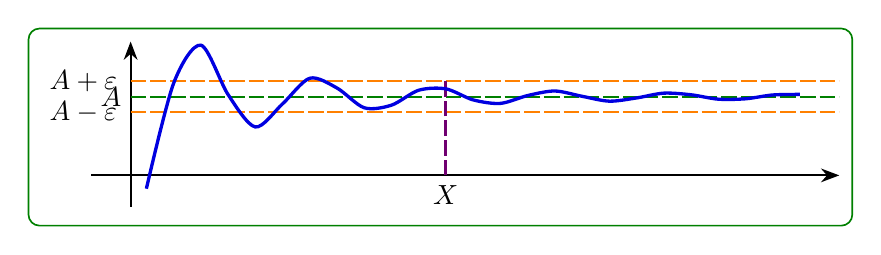
\begin{tikzpicture}[framed]
			\draw[cstaxis] (-0.5,0)--(9,0);
			\draw[cstaxis] (0,-0.4)--(0,1.7);
			\begin{scope}[visible on=<1>]
				\draw[cstdash,fourth] (0,1)--(9,1);
				\draw (-0.25,1) node {$A$};
			\end{scope}
			\begin{scope}[visible on=<2->]
				\draw[cstdash,fifth] (0,1.2)--(9,1.2);
				\draw[cstdash,fifth] (0,0.8)--(9,0.8);
				\draw[cstdash,third] (4,0)--(4,1.2);
				\draw (-0.6,1.2) node {$A+\varepsilon$};
				\draw (-0.6,0.8) node {$A-\varepsilon$};
				\draw (4,-0.25) node {$X$};
			\end{scope}
			\draw[cstcurve,main,smooth,domain=1.2:9.5] plot({\x-1},{1+3*sin(\x*240)/(1+\x*\x)});
		\end{tikzpicture}
	\end{center}

	\onslide<+->\onslide<+->
	仿造上述定义, 我们有:
	\onslide<+->
	\begin{definition}
		设 $x<-M$ 时函数 $f(x)$ 有定义.
		\onslide<+->{如果存在常数 $A$ 满足:
			\begin{center}
				\alert{$\forall\varepsilon>0, \exists X$ 使得当 $x<-X$ 时, 有 $\abs{f(x)-A}<\varepsilon$,}
			\end{center}
		}\onslide<+->{则称 $A$ 为 \emph{$f(x)$ 当 $x\ra-\infty$ 时的极限}, 记为 \emph{$\lim\limits_{x\ra-\infty}f(x)=A$}.}
	\end{definition}
\end{frame}


\begin{frame}{函数在 $\infty$ 的极限}
	\onslide<+->
	\begin{definition}
		设 $|x|>M$ 时函数 $f(x)$ 有定义.
		\onslide<+->{如果存在常数 $A$ 满足:
			\begin{center}
				\alert{$\forall\varepsilon>0, \exists X$ 使得当 $|x|>X$ 时, 有 $\abs{f(x)-A}<\varepsilon$,}
			\end{center}
		}\onslide<+->{则称 $A$ 为 \emph{$f(x)$ 当 $x\ra\infty$ 时的极限}, 记为 \emph{$\lim\limits_{x\ra\infty}f(x)=A$}.}
	\end{definition}
	\onslide<+->
	注意, 函数极限中需要分清 $x\ra\infty, x\ra+\infty, x\ra-\infty$, 而数列情形只有 $n\ra\infty$, 因为 $n$ 是正整数.

	\onslide<+->
	类似于数列极限与子数列极限的关系, 我们有
	\onslide<+->
	\begin{theorem}
		$\lim\limits_{x\ra\infty}f(x)=A \iff \lim\limits_{x\ra+\infty}f(x)=\lim\limits_{x\ra-\infty}f(x)=A$.
	\end{theorem}
\end{frame}


\begin{frame}{函数在一点的极限}
	\onslide<+->
	类似地, 当 $x$ 越来越接近 $x_0$ 时,
	\onslide<+->
	如果函数值 $f(x)$ 越来越接近常数 $A$, 则 $A$ 就是 $x\to x_0$ 时的极限.
	\onslide<+->
	\begin{center}
		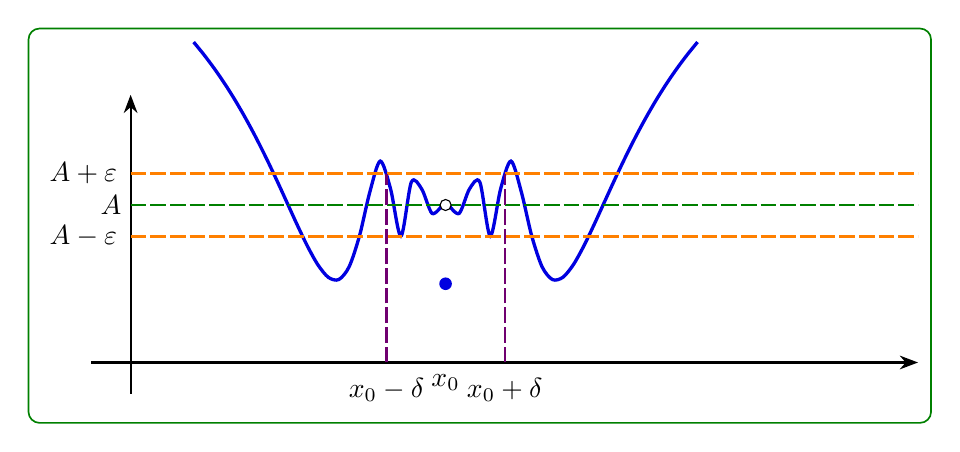
\begin{tikzpicture}[framed]
			\draw[cstaxis] (-0.5,0)--(10,0);
			\draw[cstaxis] (0,-0.4)--(0,3.4);
			\draw[cstcurve,main,smooth,domain=0.02:1.6] plot({4+2*\x},{2+1.4*\x*sin(1/\x*180)});
			\draw[cstcurve,main,smooth,domain=0.02:1.6] plot({4-2*\x},{2+1.4*\x*sin(1/\x*180)});
			\begin{scope}[visible on=<3>]
				\draw[cstdash,fourth] (0,2)--(10,2);
				\draw (-0.25,2) node {$A$};
				\draw (4,-0.25) node {$x_0$};
			\end{scope}
			\begin{scope}[visible on=<4->]
				\draw[cstdash,fifth] (0,2.4)--(10,2.4);
				\draw[cstdash,fifth] (0,1.6)--(10,1.6);
				\draw[cstdash,third] (3.25,0)--(3.25,2.4);
				\draw[cstdash,third] (4.75,0)--(4.75,2.4);
				\draw (-0.6,2.4) node {$A+\varepsilon$};
				\draw (-0.6,1.6) node {$A-\varepsilon$};
				\draw (4.75,-0.35) node {$x_0+\delta$};
				\draw (3.25,-0.35) node {$x_0-\delta$};
			\end{scope}
			\filldraw[cstdote] (4,2) circle;
			\fill[cstdot,main] (4,1) circle;
		\end{tikzpicture}
	\end{center}
\end{frame}


\begin{frame}{函数在一点的极限}
	\onslide<+->
	为了陈述方便, 我们引入去心邻域的概念.
	\onslide<+->
	\begin{definition}
	设 $\delta>0$. $x_0$ 的\emph{去心 $\delta$ 邻域}是指
		\[\Uc(x_0,\delta)=\set{x: 0<|x-x_0|<\delta}=(x_0-\delta,x_0)\cup(x_0,x_0+\delta).\]
	\end{definition}
	\onslide<+->
	\begin{definition}
		设函数 $f(x)$ 在 $x_0$ 的某个去心邻域内有定义.
		\onslide<+->{如果存在常数 $A$ 满足
		\begin{center}
			\alert{$\forall\varepsilon>0, \exists\delta>0$ 使得当 $x\in\Uc(x_0,\delta)$ 时, 有 $|f(x)-A|<\varepsilon$,}
		\end{center}
		}\onslide<+->{则称 $A$ 为 $f(x)$ 当 $x\ra x_0$ 时的极限, 记为 $\lim\limits_{x\ra x_0}f(x)=A$ 或 $f(x)\ra A(x\ra x_0)$.
		}\onslide<+->{\begin{tikzpicture}[overlay]
			\draw[semithick,third] (1.8,1.2) rectangle (12.4,1.9);
			\draw (13.4,1.55) node[third] {$\varepsilon$-$\delta$ 语言};
		\end{tikzpicture}}
	\end{definition}
\end{frame}


\begin{frame}{函数在一点的单侧极限}
	\onslide<+->
	类似地可以定义单侧极限:
	\onslide<+->
	\begin{align*}
		 \lim\limits_{x\ra x_0^+}f(x)=A&\iff\alert{\forall\varepsilon>0, \exists\delta>0\;\text{使得当}\;x\in(x_0,x_0+\delta)\;\text{时, 有}\;|f(x)-A|<\varepsilon}.\\
		\lim\limits_{x\ra x_0^-}f(x)=A&\iff\alert{\forall\varepsilon>0, \exists\delta>0\;\text{使得当}\;x\in(x_0-\delta,x_0)\;\text{时, 有}\;|f(x)-A|<\varepsilon}.
	\end{align*}
	\onslide<+->
	同样地, 我们有:
	\begin{theorem}
		$\lim\limits_{x\ra x_0}f(x)=A\iff\lim\limits_{x\ra x_0^+}f(x)=\lim\limits_{x\ra x_0^-}f(x)=A$.
	\end{theorem}
	\onslide<+->
	为了简便, 我们记 \alert{$f(x_0^+)=\lim\limits_{x\ra x_0^+}f(x)$, $f(x_0^-)=\lim\limits_{x\ra x_0^-}f(x)$}.
	\onslide<+->
	注意它们和 $f(x_0)$ 并无关系, $f$ 甚至可以在 $x_0$ 处无定义.
\end{frame}


\subsection{函数极限的证明}
\begin{frame}{例题: 函数在无穷远的极限}
	\onslide<+->
	\begin{example}
		证明 $\lim\limits_{x\ra\infty}\dfrac1x=0$.
	\end{example}
	\onslide<+->
	\begin{analysis}
		和数列极限类似, 这种问题的证明通常也分为两步:
		\begin{itemize}
			\item 估计 $|f(x)-A|$, 得到它和 $|x-x_0|<\delta$ 或 $|x|>X$ 的不等式关系. 从而求得 $\delta$ 或 $X$. 这个过程中可以进行适当的放缩.
			\item 将 $\delta$ 或 $X$ 代入极限的定义中.
		\end{itemize}
		\onslide<+->{对于本题, 从 $\Bigl|\dfrac1x-0\Bigr|<\varepsilon$ 解得 $|x|>\dfrac1\varepsilon$.}
	\end{analysis}
	\onslide<+->
	\begin{proof}
		$\forall\varepsilon>0$, 令 $X=\dfrac1\varepsilon$.
		\onslide<+->{当 $|x|>X$ 时, 有 $\Bigl|\dfrac1x-0\Bigr|=\dfrac1{|x|}<\varepsilon$.
		}\onslide<+->{所以 $\lim\limits_{x\ra\infty}\dfrac1x=0$.\qedhere}
	\end{proof}
\end{frame}


\begin{frame}{例题: 函数在无穷远的单侧极限}
	\onslide<+->
	\begin{example}
		证明 $a>1$ 时, $\lim\limits_{x\ra-\infty}a^x=0$.
	\end{example}
	\onslide<+->
	\begin{analysis}
		由于 $a>1$ 时, $\log_ax$ 是单调递增的.
		\onslide<+->{因此 $|a^x-0|=a^x<\varepsilon \iff x<\log_a \varepsilon$.}
	\end{analysis}
	\onslide<+->
	\begin{proof}
		$\forall\varepsilon>0$, 令 $X=-\log_a\varepsilon$.
		\onslide<+->{当 $x<-X$ 时, 有 $|a^x-0|=a^x<\varepsilon$.}
		
		\onslide<+->{所以 $\lim\limits_{x\ra-\infty}a^x=0$.\qedhere}
	\end{proof}
\end{frame}


\begin{frame}{例题: 函数在一点的极限}\small
	\onslide<+->
	\begin{example}
		证明 $\lim\limits_{x\ra x_0}(ax+b)=ax_0+b$.
	\end{example}
	\onslide<+->
	\begin{analysis}
		$|(ax+b)-(ax_0+b)|=a\cdot|x-x_0|<\varepsilon$, 因此我们可以取 $\delta=\varepsilon/a$.
		\onslide<+->{注意我们需要单独考虑 $a=0$ 的情形.}
	\end{analysis}
	\onslide<+->
	\begin{proof*}
		我们有 $|(ax+b)-(ax_0+b)|=a\cdot|x-x_0|$.
		\onslide<+->{如果 $a=0$, $\forall\varepsilon>0$, 令 $\delta=1$.
		}\onslide<+->{当 $0<|x-x_0|<\delta$ 时, 有 $|(ax+b)-(ax_0+b)|=0<\varepsilon$.}

		\onslide<+->{如果 $a\neq 0$, $\forall\varepsilon>0$, 令 $\delta=\dfrac\varepsilon a$.
		}\onslide<+->{当 $0<|x-x_0|<\delta$ 时, 有
			\[|(ax+b)-(ax_0+b)|=a\cdot|x-x_0|<a\delta=\varepsilon.\]
		}\onslide<+->{所以 $\lim\limits_{x\ra x_0}(ax+b)=ax_0+b$.\qedhere}
	\end{proof*}
\end{frame}


\begin{frame}{例题: 线性函数在一点的极限}
	\onslide<+->
	\begin{example}
		证明 $\lim\limits_{x\ra x_0}\sin x=\sin x_0$.
	\end{example}
	\onslide<+->
	与三角函数有关的放缩往往要用到和差化积公式
	\[\sin x-\sin y=2\sin\frac{x-y}2\cos\frac{x+y}2,\quad
	\cos x-\cos y=-2\sin\frac{x+y}2\sin\frac{x-y}2,\]
	然后将不含 $x-x_0$ 的项放缩到 $1$;
	\onslide<+->
	以及三角函数基本不等式
	\[\left|\sin x\right|\le|x|, \forall x;\qquad|x|\le\left|\tan x\right|, \forall x \in\bigl(-\frac\pi2,\frac\pi2\bigr).\]
\end{frame}


\begin{frame}{例题: 三角函数在一点的极限}
	\onslide<+->
	\begin{proof*}
		我们有
		\[\left|\sin x-\sin x_0\right|=\Bigl|2\sin\frac{x-x_0}2\cos\frac{x+x_0}2\Bigr|
			\le2\Bigl|\sin\frac{x-x_0}2\Bigr|
			\le2\Bigl|\frac{x-x_0}2\Bigr|=|x-x_0|.\]

		\onslide<+->{$\forall\varepsilon>0$, 令 $\delta=\varepsilon$.
		}\onslide<+->{当 $0<|x-x_0|<\delta$ 时, 有
		\[\left|\sin x-\sin x_0\right|\le|x-x_0|<\delta=\varepsilon.\]
		}\onslide<+->{所以 $\lim\limits_{x\ra x_0}\sin x=\sin x_0$.\qedhere}
	\end{proof*}
\end{frame}


\begin{frame}{例题: 函数在无穷远的极限}
	\onslide<+->
	\begin{example}
		证明 $\lim\limits_{x\ra\infty}\arctan x$ 不存在.
	\end{example}
	\onslide<+->
	\begin{analysis*}
		从图像上可以看出 $\lim\limits_{x\ra\pm\infty}\arctan x=\pm\dfrac\pi2$.

		\onslide<+->{我们想要使用 $|x|$ 来控制 $\Bigl|\arctan x-\dfrac\pi2\Bigr|$, 不过这个形式不容易估计.
		}\onslide<+->{令 $t=\dfrac\pi2-\arctan x$, 则问题变成了 $|x|=\Bigl|\tan\Bigl(\dfrac\pi2-t\Bigr)\Bigr|=\dfrac1{\left|\tan t\right|}$ 和 $|t|$ 的关系.
		}\onslide<+->{而我们有 $|t|\le |\tan t|$.}

		\onslide<+->{我们还需要估计 $t$ 的范围.
		}\onslide<+->{由于我们考虑的是 $x\ra+\infty$, 不妨设 $x>0$,
		}\onslide<+->{那么
		\[\arctan x \in\Bigl(0,\frac\pi2\Bigr),\qquad t=\frac\pi2-\arctan x\in\Bigl(0,\frac\pi2\Bigr).\]}
		\vspace{-\baselineskip}
	\end{analysis*}
\end{frame}


\begin{frame}{例题: 函数在无穷远的极限}
	\begin{proof*}
		我们来证明 $\lim\limits_{x\ra+\infty}\arctan x=\dfrac\pi2$.
		\onslide<+->{当 $x>0$ 时, $0<\dfrac\pi2-\arctan x<\dfrac\pi2$.
		}\onslide<+->{因此
			\[\Bigl|\frac\pi2-\arctan x\Bigr|
			\le\Bigl|\tan\Bigl(\frac\pi2-\arctan x\Bigr)\Bigr|
			=\frac1{\left|\tan(\arctan x)\right|}=\frac1{|x|}.\]
		}\onslide<+->{$\forall\varepsilon>0$, 令 $X=\dfrac1\varepsilon>0$.
		}\onslide<+->{当 $x>X$ 时, 有
		\[\Bigl|\frac\pi2-\arctan x\Bigr|\le\frac1{|x|}<\frac1X=\varepsilon.\]
		}\onslide<+->{所以 $\lim\limits_{x\ra+\infty}\arctan x=\dfrac\pi2$.}

		\onslide<+->{类似可证, $\lim\limits_{x\ra-\infty}\arctan x=-\dfrac\pi2$.
		}\onslide<+->{因此 $\lim\limits_{x\ra\infty}\arctan x$ 不存在.\qedhere}
	\end{proof*}
\end{frame}


\begin{frame}{例题: 有理函数在一点的极限}\small
	\beqskip{2pt}
	\onslide<+->
	\begin{example}
		证明 $\lim\limits_{x\ra2}\dfrac{x^2-4}{x-2}=4$.
	\end{example}
	\onslide<+->
	\begin{analysis}
		这种极限是 $\dfrac fg$ 型, 其中 $f\ra0, g\ra0$.
		\onslide<+->{我们称之为 \emph{$\dfrac00$ 型不定式}.
		}\onslide<+->{它的极限可能存在, 可能不存在.
		}\onslide<+->{这种一般要去掉公因式, 将其变为定式.}
	\end{analysis}
	\onslide<+->
	\begin{proof}
		$\displaystyle \biggl|\frac{x^2-4}{x-2}-4\biggr|=|x+2-4|=|x-2|$.
		\onslide<+->{$\forall\varepsilon>0$, 令 $\delta=\varepsilon$.
		}\onslide<+->{当 $0<|x-2|<\delta$ 时, 有
		\[\biggl|\frac{x^2-4}{x-2}-4\biggr|=|x-2|<\varepsilon.\]
		}\onslide<+->{所以 $\lim\limits_{x\ra2}\dfrac{x^2-4}{x-2}=4$.\qedhere}
	\end{proof}
	\endgroup
\end{frame}


\begin{frame}{例题: 分段函数求待定参数}
	\onslide<+->
	\begin{example}
		如果函数 $f(x)=\begin{cases}
			a\sin x,&x<\pi/2;\\
			x+b,&x>\pi/2
		\end{cases}$ 满足 $\lim\limits_{x\ra\pi/2}f(x)=1$, 求 $a,b$.
	\end{example}
	\onslide<+->
	\begin{analysis*}
		本题是典型的由分段函数性质求待定参数的问题, 我们后续会经常遇到.
		\onslide<+->{由于一点处极限等价于两侧极限都存在且为 $1$, 因此我们会得到两个等式, 从而可以解出两个未知参数.}

		\onslide<+->{由于 $f(x)$ 的两个分段都是我们已经求过极限的函数, 因此我们可以直接用前面已经证明的结论.}
	\end{analysis*}
	\onslide<+->
	\begin{solution}
		由于 $\displaystyle f\Bigl[\bigl(\frac\pi2\bigr)^+\Bigr]=\frac\pi2+b,\ 
		f\Bigl[\bigl(\frac\pi2\bigr)^-\Bigr]=a\sin\frac\pi2=a$,
		\onslide<+->{因此 $a=1, b=1-\dfrac\pi2$.}
	\end{solution}
\end{frame}


\begin{frame}{例题: 取整函数的极限}
	\beqskip{7pt}
	\onslide<+->
	\begin{example}
		对于哪些 $x_0$, $\lim\limits_{x\ra x_0}[x]$ 存在.
	\end{example}
	\onslide<+->
	\begin{analysis*}
		与 $[x]$ 有关的问题往往需要用到两个不等式
		\begin{center}
			\alert{$[x]\le x<x+1$} 或 \alert{$x-1<[x]\le x$}.
		\end{center}

		\onslide<+->{从 $[x]$ 的图像上可以看出 $x_0\in\BZ$ 时左右极限不相等, 从而极限不存在.
		}\onslide<+->{解答时, 我们取 $x_0$ 的 $\delta=1/2$ 邻域, 则在这个邻域的左右各自半边内, $[x]$ 是常值函数, 从而得到单侧极限.}

		\onslide<+->{当 $x_0\notin \BZ$ 时, 我们同样希望取一个小邻域使得 $[x]$ 是常值函数.
		}\onslide<+->{这需要 $\delta$ 不超过 $x_0$ 和两边的最近的整数的距离.
		}\onslide<+->{所以
		\[\delta=\min\set{x_0-[x_0], [x_0]+1-x_0}.\]}
		\vspace{-\baselineskip}
	\end{analysis*}
	\endgroup
\end{frame}


\begin{frame}{例题: 取整函数的极限}
	\onslide<+->
	\begin{solution*}
		如果 $x_0\in\BZ$, 则
		\begin{itemize}
			\item 当 $x\in(x_0, x_0+1/2)$ 时, $[x]=x_0$, 所以 $\lim\limits_{	x\ra x_0^+}[x]=x_0$;
			\item 当 $x\in(x_0-1/2, x_0)$ 时, $[x]=x_0-1$, 所以 $\lim\limits_{	x\ra x_0^-}[x]=x_0-1$.
		\end{itemize}
		\onslide<+->{因此 $\lim\limits_{x\ra x_0}[x]$ 不存在.}

		\onslide<+->{如果 $x_0\notin\BZ$, 令 $\delta=\min\set{x_0-[x_0], [x_0]+1-x_0}>0$.
		}\onslide<+->{name 
		\[[x_0]\le x_0-\delta<x_0+\delta\le[x_0]+1.\]
		}\onslide<+->{当 $0<|x-x_0|<\delta$ 时, 有 $x_0-\delta<x<x_0+\delta$,
		}\onslide<+->{从而 $[x_0]<x<[x_0]+1$, $[x]=x_0$.
		}\onslide<+->{因此 $\lim\limits_{x\ra x_0}[x]=x_0$.}

		\onslide<+->{故当且仅当 $x_0\notin\BZ$ 时, $\lim\limits_{x\ra x_0}[x]$ 存在.}
	\end{solution*}
\end{frame}

\section{初等函数}

\subsection{指数函数}

\begin{frame}{指数函数}
	\onslide<+->
	我们将实变函数中的初等函数推广到复变函数.
	\onslide<+->
	多项式函数和有理函数的解析性质已经介绍过, 这里不再重复.
	\onslide<+->
	现在我们来定义指数函数.

	\onslide<+->
	指数函数有多种等价的定义方式:
	\begin{enumerate}
		\item $\exp z=\ee^x(\cos y+\ii\sin y)$ (欧拉恒等式);
		\item $\exp z=\liml_{n\to\infty}\Bigl(1+\dfrac zn\Bigr)^n$ (极限定义);
		\item $\exp z=1+z+\dfrac{z^2}{2!}+\dfrac{z^3}{3!}+\cdots
		=\liml_{n\to\infty}\sum\limits_{k=0}^n\dfrac{z^k}{k!}$ (级数定义);
		\item $\exp z$ 是唯一的一个处处解析的函数, 使得当 $z=x\in\BR$ 时, $\exp z=\ee^x$ ($\ee^x$ 的解析延拓).
	\end{enumerate}
\end{frame}


\begin{frame}{指数函数与欧拉恒等式}
	\onslide<+->
	有些人会从 $\ee^x,\cos x,\sin x$ 的泰勒展开
	\begin{align*}
		\ee^x&=1+x+\frac{x^2}{2!}+\frac{x^3}{3!}+\cdots\\
		\cos x&=1-\frac{x^2}{2!}+\frac{x^4}{4!}+\cdots\\
		\sin x&=x-\frac{x^3}{3!}+\frac{x^5}{5!}\cdots
	\end{align*}
	形式地带入得到欧拉恒等式 $\ee^{\ii x}=\cos x+\ii\sin x$.
	\onslide<+->
	事实上我们可以把它当做复指数函数的定义, 而不是欧拉恒等式的证明.
	\onslide<+->
	我们将在第四章说明\enumnum1、\enumnum3和\enumnum4是等价的.
\end{frame}



\begin{frame}{指数函数的定义}
	\onslide<+->
	我们来证明\enumnum1和\enumnum2等价.
	\onslide<+->
	\begin{align*}
		\lim_{n\to\infty}\Bigabs{1+\frac zn}^n
		&=\lim_{n\to\infty}\Bigl(1+\frac{2x}n+\frac{x^2+y^2}{n^2}\Bigr)^{\frac n2}\quad
		\visible<+->{(1^\infty\ \text{型不定式})}\\
		&\visible<+->{=\exp\left[\lim_{n\to\infty}\frac n2
		\Bigl(\frac{2x}n+\frac{x^2+y^2}{n^2}\Bigr)\right]=\ee^x.}
	\end{align*}
	\onslide<+->
	不妨设 $n>\abs{z}$, 这样 $1+\dfrac zn$ 落在右半平面,
	\onslide<+->
	\[
		\lim_{n\to\infty} n\arg{\Bigl(1+\frac zn\Bigr)}
		=\lim_{n\to\infty} n\arctan \frac y{n+x}
		\visible<+->{=\lim_{n\to\infty}\frac{ny}{n+x}=y.}
	\]
	\bigdel
	\onslide<+->
	故 $\exp z=\ee^x(\cos y+\ii\sin y)$.
\end{frame}


\begin{frame}{指数函数的性质}
	\onslide<+->
	\begin{definition*}[][指数函数]
	\[
		\exp z:=\ee^x(\cos y+\ii\sin y).
	\]
	\end{definition*}
	\onslide<+->
	为了方便, 我们也记 $\emphm{\ee^z=\exp z}$.
	\onslide<+->
	指数函数有如下性质:
	\begin{itemize}\bf
		\item $\exp z$ 处处解析, 且 $(\exp z)'=\exp z$.
		\item $\exp z\neq 0$.
		\item $\exp(z_1+z_2)=\exp z_1\cdot \exp z_2$.
		\item $\exp(z+2k\pi\ii)=\exp z$, 即 $\exp z$ 周期为 $2\pi\ii$.
		\item $\exp z_1=\exp z_2$ 当且仅当 $z_1=z_2+2k\pi\ii,k\in\BZ$.
		\item 指数函数将直线族 $\Re z=c$ 映为圆周族 $\abs{w}=\ee^c$, 将直线族 $\Im z=c$ 映为射线族 $\Arg w=c$.
	\end{itemize}
\end{frame}


\begin{frame}{指数函数的性质}
	\onslide<+->
	\begin{example}
		计算函数 $f(z)=\exp(z/6)$ 的周期.
	\end{example}

	\onslide<+->
	\begin{solution}
		设 $f(z_1)=f(z_2)$, 则 $\ee^{z_1/6}=\ee^{z_2/6}$.
		\onslide<+->{%
			因此存在 $k\in\BZ$ 使得
			\[
				\frac{z_1}6=\frac{z_2}6+2k\pi\ii,
			\]
		}\onslide<+->{%
			从而 $z_1-z_2=12k\pi\ii$.
		}\onslide<+->{%
			所以 $f(z)$ 的周期是 $12\pi\ii$.
		}
	\end{solution}

	\onslide<+->
	一般地, $\exp(az+b)$ 的周期是 $\dfrac{2\pi\ii}a$ (或写成 $-\dfrac{2\pi\ii}a$), $a\neq 0$.
\end{frame}


\subsection{对数函数}

\begin{frame}{对数函数}
	\onslide<+->
	对数函数 $\Ln z$ 定义为指数函数 $\exp z$ 的反函数.
	\onslide<+->
	为什么我们用大写的 $\Ln$ 呢? 
	\onslide<+->
	在复变函数中, 很多函数是多值函数.
	\onslide<+->
	为了便于研究, 我们会固定它的一个单值分支.
	\onslide<+->
	我们将多值的这个开头字母大写, 而对应的单值的则是开头字母小写.
	\onslide<+->
	例如 $\Arg z$ 和 $\arg z$.

	\onslide<+->
	设 $z\neq0,\ee^w=z=r\ee^{\ii\theta}=\ee^{\ln r+\ii\theta}$,
	\onslide<+->
	则
	\[w=\ln r+\ii\theta+2k\pi\ii,\quad k\in\BZ.
	\]
\end{frame}


\begin{frame}{对数函数及其主值}
	\onslide<+->
	\begin{definition*}{对数函数}
		\begin{enumerate}
			\item 定义\emph{对数函数}
			\[
				\Ln z=\ln\abs{z}+\ii\Arg z.
			\]
			它是一个多值函数.
			\item 定义\emph{对数函数主值}
			\[
				\ln z=\ln\abs{z}+\ii\arg z.
			\]
			\bigdel
		\end{enumerate}
	\end{definition*}

	\onslide<+->
	对于每一个整数 $k$, $\ln z+2k\pi\ii$ 都给出了 $\Ln z$ 的一个单值分支.
	\onslide<+->
	特别地, 当 $z=x>0$ 是正实数时, $\ln z$ 就是实变的对数函数.
\end{frame}


\begin{frame}{例题: 对数函数的计算}
	\onslide<+->
	\begin{example}
		求 $\Ln 2,\Ln(-1)$ 以及它们的主值.
	\end{example}

	\onslide<+->
	\begin{solution}
		\begin{enumerate}
			\item
			\[
				\Ln2=\ln2+2k\pi\ii, k\in\BZ,
			\]
			\onslide<+->{%
				主值为 $\ln 2$.
			}
			\item
			\[
				\Ln(-1)=\ln1+\ii\Arg(-1)=(2k+1)\pi\ii, k\in\BZ,
			\]
			\onslide<+->{%
				主值为 $\pi\ii$.
			}
		\end{enumerate}
	\end{solution}
\end{frame}


\begin{frame}{例题: 对数函数的计算}
	\beqskip{5pt}
	\onslide<+->
	\begin{example}
	求 $\Ln(-2+3\ii),\Ln(3-\sqrt3 i)$.
	\end{example}

	\onslide<+->
	\begin{solution}
		\begin{enumerate}
			\item
			\begin{align*}
				\Ln(-2+3\ii)&=\ln\abs{-2+3\ii}+\ii\Arg(-2+3\ii)\\
				&\visible<+->{=\frac 12\ln 13+\Bigl(-\arctan\frac 32+\pi+2k\pi\Bigr)\ii,\quad k\in\BZ.}
			\end{align*}
			\item
			\begin{align*}
				\Ln(3-\sqrt3\ii)&=\ln\abs{3+\sqrt 3\ii}+\ii\Arg(3-\sqrt 3\ii)\\
				&\visible<+->{=\ln 2\sqrt 3+\Bigl(-\frac\pi6+2k\pi\Bigr)\ii
				=\ln 2\sqrt 3+\Bigl(2k-\frac16\Bigr)\pi\ii,\quad k\in\BZ.}
			\end{align*}
		\end{enumerate}
		\vspace{-.5\baselineskip}
	\end{solution}
	\endgroup
\end{frame}


\begin{frame}{例题: 对数函数的计算}
	\onslide<+->
	\begin{example}
		解方程 $\ee^z-1-\sqrt 3\ii=0$.
	\end{example}

	\onslide<+->
	\begin{solution}
		由于 $1+\sqrt 3 i=2\ee^{\frac{\pi\ii}3}$,
		\onslide<+->{%
			因此
			\[
				z=\Ln(1+\sqrt 3\ii)=\ln 2+\Bigl(2k+\frac13\Bigr)\pi\ii,\quad k\in\BZ.
			\]
		}\bigdel
	\end{solution}

	\onslide<+->
	\begin{exercise}
		求 $\ln(-1-\sqrt3\ii)=$\fillblankframe[2cm][3mm]{$\ln 2-\dfrac{2\pi\ii}3$}.
	\end{exercise}
\end{frame}


\begin{frame}{对数函数的性质}
	\onslide<+->
	对数函数与其主值的关系是
	\[
		\emphn{\Ln z=\ln z+\Ln 1=\ln z+2k\pi\ii,\quad k\in\BZ}.
	\]

	\onslide<+->
	根据辐角以及辐角主值的相应等式, 我们有
	\[
		\Ln(z_1\cdot z_2)=\Ln z_1+\Ln z_2,\quad
		\Ln\frac{z_1}{z_2}=\Ln z_1-\Ln z_2,
	\]
	\[
		\Ln \sqrt[n]z=\dfrac1n\Ln z.
	\]
	\onslide<+->
	而当 $\abs{n}\ge 2$ 时, \alert{$\Ln z^n=n\Ln z$ 不成立}.
	\onslide<+->
	以上等式换成 $\ln z$ 均未必成立.
\end{frame}


\begin{frame}{对数函数的导数}
\beqskip{1pt}
	\onslide<+->
	设 $x$ 是正实数, 
	\onslide<+->
	则
	\[
		\ln (-x)=\ln x+\pi\ii,\quad
		\lim_{y\to0^-}\ln (-x+y\ii)=\ln x-\pi\ii,
	\]
	\onslide<+->
	因此 $\ln z$ 在负实轴和零处不连续.

	\onslide<+->
	而在其它地方 $-\pi<\arg z<\pi$, $\ln z$ 是 $\ee^z$ 在区域 $-\pi<\Im z<\pi$ 上的单值反函数, 
	\onslide<+->
	从而
	\alert{$(\ln z)'=\dfrac 1z$},
	\alert{$\ln z$ 在除负实轴和零处的区域解析}.

	\onslide<+->
	也可以通过C-R方程来得到 $\ln z$ 的解析性和导数: 当 $x>0$ 时,
	\[
		\ln z=\half \ln(x^2+y^2)+\ii\arctan \frac yx,
	\]
	\onslide<+->
	\[
		u_x=v_y=\frac x{x^2+y^2},\qquad v_x=-u_y=-\frac y{x^2+y^2},
	\]
	\[
		(\ln z)'=\frac{x-yi}{x^2+y^2}=\frac 1z.
	\]
	其它情形可取虚部为 $\arccot\dfrac xy$ 或 $\arccot\dfrac xy-\pi$ 类似证明.
\endgroup
\end{frame}


\subsection{幂函数}

\begin{frame}{幂函数的性质: $a$ 为整数时}
	\onslide<+->
	\begin{definition*}[][幂函数]
		\begin{enumerate}
			\item 设 $a\neq 0$, $z\neq 0$, 定义\emph{幂函数}
			\[
				w=z^a=\ee^{a\Ln z}
				=\exp\bigl[a\ln\abs{z}+\ii a(\arg z+2k\pi)\bigr],\quad k\in\BZ.
			\]
			\item \emph{幂函数的主值}为
			\[
				w=\ee^{a\ln z}=\exp\bigl(a\ln\abs{z}+\ii a\arg z\bigr).
			\]
		\end{enumerate}
		\bigdel
	\end{definition*}
	\onslide<+->
	根据 $a$ 的不同, 这个函数有着不同的性质.

	\onslide<+->
	当 $a$ 为整数时, 因为 $\ee^{2ak\pi\ii}=1$, 所以 $w=z^a$ 是单值的.
	\onslide<+->
	此时 $z^a$ 就是我们之前定义的乘幂.

	\onslide<+->
	当 $a$ 是非负整数时, $z^a$ 在复平面上解析;
	\onslide<+->
	当 $a$ 是负整数时, $z^a$ 在 $\BC-\{0\}$ 上解析.
\end{frame}


\begin{frame}{幂函数的性质: $a$ 为分数时}
	\onslide<+->
	当 $a=\dfrac pq$ 为分数, $p,q$ 为互质的整数且 $q>1$ 时,
	\onslide<+->
	\[
		z^{\frac pq}=\abs{z}^{\frac pq}\exp\left[\frac{\ii p(\arg z+2k\pi)}q\right],\quad k=0,1,\dots,q-1
	\]
	具有 $q$ 个值.
	\onslide<+->
	去掉负实轴和 $0$ 之后, 它的主值 $w=\exp(a\ln z)$ 是处处解析的.
	\onslide<+->
	事实上它就是 $\sqrt[q]{z^p}=(\sqrt[q]z)^p$.
	\onslide<+->
	\begin{center}
		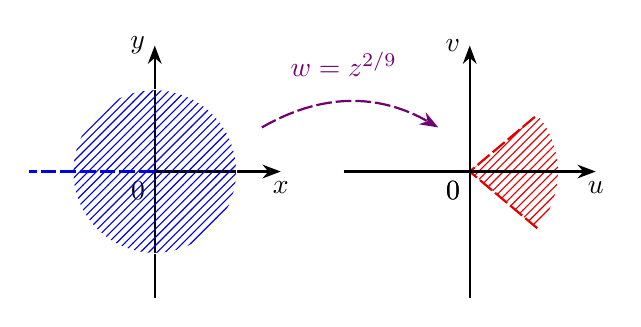
\begin{tikzpicture}[scale=.8]
			\coordinate [label=below left:{$0$}] (O) at (0,0);
			\coordinate [label=below:{$x$}] (X) at (2,0);
			\coordinate [label=left:{$y$}] (Y) at (0,2);
			\draw[cstaxis] (O)--(X);
			\draw[cstaxis] (0,-2)--(Y);
			\draw[draw=white,cstfille1] (O) circle (1.3);
			\draw[cstdash,main] (0,0)--(-2,0);
			\draw[cstdash,cstra,third] (1.7,.7)to [bend left] (4.5,.7);
			\draw (3,1.7) node[third] {$w=z^{2/9}$};
			\begin{scope}[xshift=5cm]
				\coordinate [label=below left:{$0$}] (O) at (0,0);
				\fill[cstfille2,pattern color=second] (O)--({1.4*cos(40)},{1.4*sin(40)}) arc (40:-40:1.4)--cycle;
				\draw[cstdash,second] ({1.4*cos(40)},{-1.4*sin(40)})--(0,0)--({1.4*cos(40)},{1.4*sin(40)});
				\coordinate [label=below left:{$0$}] (O) at (0,0);
				\coordinate [label=below:{$u$}] (X) at (2,0);
				\coordinate [label=left:{$v$}] (Y) at (0,2);
				\draw[cstaxis] (-2,0)--(X);
				\draw[cstaxis] (0,-2)--(Y);
			\end{scope}
		\end{tikzpicture}
	\end{center}
\end{frame}


\begin{frame}{幂函数的性质: $a$ 为其他情形}
\onslide<+->
	对于其它的 $a$, $z^a$ 具有无穷多个值.
	\onslide<+->
	这是因为此时当 $k\neq0$ 时, $2k\pi a \ii$ 不可能是 $2\pi\ii$ 的整数倍. 
	\onslide<+->
	从而不同的 $k$ 得到的是不同的值.
	\onslide<+->
	去掉负实轴和 $0$ 之后,
	\onslide<+->
	它的主值 $w=\exp(a\ln z)$ 也是处处解析的.
	\onslide<+->
	\begin{center}
		\arrayrulecolor{second}
		\begin{tabular}{cccc} \toprule
			$a$& $z^a$ 的值& $z^a$ 的解析区域\\ \midrule
			&&$n\ge0$ 时处处解析\\
			\multirow{-2}*{整数 $n$}&\multirow{-2}*{单值}&$n<0$ 时除零点外解析\\ \midrule
			分数 $p/q$&$q$ 值&除负实轴和零点外解析\\ \midrule
			无理数或虚数&无穷多值&除负实轴和零点外解析\\ \bottomrule
		\end{tabular}
	\end{center}
\end{frame}


\begin{frame}{典型例题: 幂函数的计算}
	\onslide<+->
	\begin{example}
		求 $1^{\sqrt 2}$ 和 $\ii^\ii$.
	\end{example}
	\onslide<+->
	\begin{solution}
		\[
			1^{\sqrt2}=\ee^{\sqrt2\Ln1}
			\visible<+->{=\ee^{\sqrt 2\cdot 2k\pi\ii}}
			\visible<+->{=\cos(2\sqrt 2k\pi)+\ii\sin(2\sqrt 2k\pi), k\in\BZ.}
		\]
		\onslide<+->{%
			\[
				\ii^\ii=\ee^{\ii\Ln \ii}
				\visible<+->{=\exp\left[\ii\cdot\Bigl(2k+\half\Bigr)\pi\ii\right]}
				\visible<+->{=\exp\Bigl(-2k\pi-\half\pi\Bigr), k\in\BZ.}
			\]
		}\bigdel
	\end{solution}
	\onslide<+->
	\begin{exercise}
		$3^\ii$ 的辐角主值是\fillblankframe{$\ln 3$}.
	\end{exercise}
\end{frame}


\begin{frame}{幂函数的性质}
	幂函数与其主值有如下关系:
	\onslide<+->
	\[
		\emphn{z^a=\ee^{a\ln z}\cdot 1^a
		=\ee^{a\ln z}\cdot \ee^{2ak\pi\ii},\quad k\in\BZ.}
	\]

	\onslide<+->
	对于幂函数的主值,
	\[
		\alertn{(z^a)'}=\Bigl(\ee^{a\ln z}\Bigr)'=\frac{a\ee^{a\ln z}}z=\alertn{az^{a-1}}.
	\]

	\onslide<+->
	一般而言, $z^a\cdot z^b=z^{a+b}$ 和 $(z^a)^b=z^{ab}$ 都是不成立的.

	\onslide<+->
	最后, 注意 $\ee^a$ 作为指数函数 $f(z)=\ee^z$ 在 $a$ 处的值和作为 $g(z)=z^a$ 在 $e$ 处的值是\alert{不同}的.
	\onslide<+->
	因为后者在 $a\not\in\BZ$ 时总是多值的.
	\onslide<+->
	前者实际上是后者的主值.
	\onslide<+->
	为避免混淆, 以后我们总\alert{默认 $\ee^a$ 表示指数函数 $\exp a$}.
\end{frame}


\subsection{三角函数和反三角函数}

\begin{frame}{三角函数的定义}
	\onslide<+->
	我们知道
	\[
		\cos x=\frac{\ee^{\ii x}+\ee^{-\ii x}}2,\quad
		\sin x=\frac{\ee^{\ii x}-\ee^{-\ii x}}{2\ii}
	\]
	对于任意实数 $x$ 成立,
	\onslide<+->
	我们将其推广到复数情形.
	\onslide<+->
	\begin{definition*}[][余弦和正弦函数]
		\[
			\cos z=\frac{\ee^{\ii z}+\ee^{-\ii z}}2,\quad
			\sin z=\frac{\ee^{\ii z}-\ee^{-\ii z}}{2\ii}.
		\]
	\end{definition*}
	\onslide<+->
	那么欧拉恒等式 \emph{$\ee^{\ii z}=\cos z+\ii\sin z$ 对任意复数 $z$ 均成立}.
\end{frame}


\begin{frame}{三角函数的性质}
	\onslide<+->
	不难得到
	\[
		\cos(\ii y)=\dfrac{\ee^y+\ee^{-y}}2,\qquad
		\visible<+->{\sin(\ii y)=\ii\dfrac{\ee^y-\ee^{-y}}2.}
	\]
	\onslide<+->
	当 $y\to\infty$ 时, $\cos(\ii y)$ 和 $\sin(\ii y)$ 都 $\to\infty$.
	\onslide<+->
	因此 \alert{$\sin z$ 和 $\cos z$ 并不有界}. 
	\onslide<+->
	这和实变情形完全不同.

	\onslide<+->
	容易看出 $\cos z$ 和 $\sin z$ 的零点都是实数.
	\onslide<+->
	于是我们可类似定义其它三角函数
	\begin{align*}
		\alertn{\tan z}&
		\alertn{=\frac{\sin z}{\cos z},z\neq\Bigl(k+\half\Bigr)\pi,}&
		\alertn{\cot z}&
		\alertn{=\frac{\cos z}{\sin z},z\neq k\pi,}\\
		\alertn{\sec z}&
		\alertn{=\frac{1}{\cos z},z\neq\Bigl(k+\half\Bigr)\pi,}&
		\alertn{\csc z}&
		\alertn{=\frac{1}{\sin z},z\neq k\pi.}
	\end{align*}
\end{frame}


\begin{frame}{三角函数的性质}
	\onslide<+->
	这些三角函数的奇偶性, 周期性和导数与实变情形类似,
	\[
		\alertn{(\cos z)'=-\sin z,\quad
		(\sin z)'=\cos z,}
	\]
	\onslide<+->
	且在定义域范围内是处处解析的.

	\onslide<+->
	三角函数的各种恒等式在复数情形也仍然成立,
	\onslide<+->
	例如
	\begin{itemize}
		\item $\cos(z_1\pm z_2)=\cos z_1 \cos z_2\mp \sin z_1 \sin z_2$,
		\item $\sin(z_1\pm z_2)=\sin z_1 \cos z_2\pm\cos z_1 \sin z_2$,
		\item $\sin^2z+\cos^2z=1$.
	\end{itemize}
\end{frame}


\begin{frame}{双曲函数}
	\onslide<+->
	类似的, 我们可以定义双曲函数:
	\onslide<+->
	\[
		\alertn{\ch z=\frac{\ee^z+\ee^{-z}}2=\cos \ii z,}
	\]
	\onslide<+->
	\[
		\alertn{\sh z=\frac{\ee^z-\ee^{-z}}2=-\ii \sin \ii z,}
	\]
	\onslide<+->
	\[
		\alertn{\tanh z=\frac{\ee^z-\ee^{-z}}{\ee^z+\ee^{-z}}
		=-\ii \tan \ii z,\quad z\neq \Bigl(k+\half\Bigr)\pi\ii.}
	\]
	\onslide<+->
	它们的奇偶性和导数与实变情形类似, 在定义域范围内是处处解析的.

	\onslide<+->
	$\ch z,\sh z$ 的周期是 $2\pi\ii$, $\tanh z$ 的周期是 $\pi\ii$.
\end{frame}


\begin{frame}{反三角函数和反双曲函数}
	\onslide<+->
	设 $z=\cos w=\dfrac{\ee^{\ii w}+\ee^{-\ii w}}2$,
	\onslide<+->
	则
	\[
		\ee^{2\ii w}-2z\ee^{\ii w}+1=0,\quad
		\visible<+->{\ee^{\ii w}=z+\sqrt{z^2-1}\ \text{(双值)}.}
	\]
	\onslide<+->
	因此\emph{反余弦函数}为
	\[
		w=\Arccos z=-\ii \Ln(z+\sqrt{z^2-1}).
	\]
	\onslide<+->
	显然它是多值的.
	\onslide<+->
	同理, 我们有:
	\begin{itemize}
		\item \emph{反正弦函数} $\Arcsin z=-\ii \Ln(\ii z+\sqrt{1-z^2})$;
		\item \emph{反正切函数} $\Arctan z=-\dfrac \ii2\Ln\dfrac{1+\ii z}{1-\ii z}, z\neq \pm \ii$;
		\item \emph{反双曲余弦函数} $\Arch z=\Ln(z+\sqrt{z^2-1})$;
		\item \emph{反双曲正弦函数} $\Arsh z=\Ln(z+\sqrt{z^2+1})$;
		\item \emph{反双曲正切函数} $\Arth z=\dfrac12\Ln\dfrac{1+z}{1-z}, z\neq \pm1$.
	\end{itemize}
\end{frame}


\begin{frame}{例题: 解三角函数方程}
	\onslide<+->
	\begin{example}
		解方程 $\sin z=2$.
	\end{example}
	\onslide<+->
	\begin{solution}
	由于 $\sin z=\dfrac{\ee^{\ii z}-\ee^{-\ii z}}{2\ii}=2$,
	\onslide<+->{%
		我们有
		\[
			\ee^{2\ii z}-4\ii\ee^{\ii z}-1=0.
		\]
	}\onslide<+->{%
		于是 $\ee^{\ii z}=(2\pm\sqrt 3)\ii$,
	}\onslide<+->{%
		\[
			z=-\ii \Ln[(2\pm\sqrt 3)\ii]=\Bigl(2k+\half\Bigr)\pi\pm \ii\ln(2+\sqrt3),\quad k\in\BZ.
		\]
	}\bigdel
	\end{solution}
\end{frame}

\begin{frame}{例题: 解三角函数方程}
	\onslide<+->
	\begin{solution}[][另解]
	由 $\sin z=2$ 可知
	\[
		\cos z=\sqrt{1-\sin^2 z}=\pm\sqrt 3\ii.
	\]
	\onslide<+->{%
		于是 $\ee^{\ii z}=\cos z+\ii\sin z=(2\pm\sqrt 3)\ii$,
	}\onslide<+->{%
		\[
			z=-\ii \Ln[(2\pm\sqrt 3)\ii]=\Bigl(2k+\half\Bigr)\pi\pm \ii\ln(2+\sqrt3),\quad k\in\BZ.
		\]
	}\bigdel
	\end{solution}
	\onslide<+->
	对于任意 $z$, 总存在 $\theta$ 使得
	\begin{align*}
		\Arcsin z&=(2k+\half)\pi\pm \theta,\\
		\Arccos z&=2k\pi\pm \theta,\\
		\Arctan z&=k\pi+\theta,\quad (z\ne\pm\ii).
	\end{align*}
\end{frame}


\subsection{在有理函数的应用}


\begin{frame}{有理函数分拆}
	\onslide<+->
	称分子次数小于分母次数的有理函数为\emph{真分式}.
	\onslide<+->
	任何一个有理函数 $f(z)$ 都可以通过带余除法分解为一个多项式 $g(z)$ 和一个真分式之和.

	\onslide<+->
	若这个有理函数分母的零点均能求出, 则这个真分式又可以分拆为部分分式之和, 其中\emph{部分分式}是指形如 $\dfrac{a}{(x-b)^k}$ 的真分式.
	\onslide<+->
	我们来介绍求这种分拆的一种方法.
\end{frame}


\begin{frame}{例题: 有理函数分拆}
	\beqskip{2pt}
	\onslide<+->
	\begin{example}[near]
		将 $f(z)=\dfrac{1}{(z-1)(z-2)^2}$ 展开成部分分式之和.
	\end{example}
	\onslide<+->
	\begin{solution}[near]
		设 $f(z)=\dfrac{a}{z-1}+\dfrac{b}{z-2}+\dfrac{c}{(z-2)^2}$,
		\onslide<+->{%
			则
			\begin{align*}
				a&=\lim_{z\ra1} (z-1)f(z)
					=\lim_{z\ra1} \frac{1}{(z-2)^2}
					=1,\\
				\onslide<+->{b}&\onslide<.->{=\lim_{z\ra2} \bigl((z-2)^2f(z)\bigr)'
					=\lim_{z\ra2} \Bigl(\frac{1}{z-1}\Bigr)'
					=-1,}\\
				\onslide<+->{c}&\onslide<.->{=\lim_{z\ra2} (z-2)^2f(z)
					=\lim_{z\ra2} \frac{1}{z-1}=1.}
			\end{align*}
		}\onslide<+->{%
			因此
			\[
				f(z)=\frac{1}{z-1}-\frac{1}{z-2}+\frac{1}{(z-2)^2}.
			\]
		}\bigdel
	\end{solution}
	\endgroup
\end{frame}


\begin{frame}{有理函数的导数\noexer}
	\onslide<+->
	得到这种分拆之后, 我们可以求出该有理函数的任意阶导数.
	\onslide<+->
	\begin{example}[nearnext]
		计算 $f(x)=\dfrac1{1+x^2}$ 的 $n$ 阶导数.
	\end{example}
	\onslide<+->
	\begin{solution}[nearprev]
		设
		\[
			f(z)
			=\frac1{1+z^2}
			=\frac \ii2\biggl(\frac1{z+\ii}-\frac1{z-\ii}\biggr),
		\]
		\onslide<+->{%
			则它在除 $z=\pm \ii$ 外处处解析,
		}\onslide<+->{%
			且
			\begin{align*}
				f^{(n)}(z)&
				=\frac \ii2\biggl(\frac1{z+\ii}-\frac1{z-\ii}\biggr)^{(n)}
				\onslide<+->{=\frac \ii2\cdot(-1)^n n!\biggl(\frac1{(z+\ii)^{n+1}}-\frac1{(z-\ii)^{n+1}}\biggr)}\\&
				\onslide<+->{=(-1)^{n+1}n!\Im{(z+\ii)^{-n-1}}.}
			\end{align*}
		}\bigdel
	\end{solution}
\end{frame}
	
	
\begin{frame}{有理函数的导数}
	\onslide<+->
	\begin{solution}[][]%
		当 $z=x$ 为实数时,
		\[
			\abs{x+\ii}=\sqrt{x^2+1},\qquad
			\arg(x+\ii)=\arccot x,
		\]
		\onslide<+->{%
			于是
			\[
				\frac1{(z\pm\ii)^{n+1}}=(x^2+1)^{-\frac{n+1}2}\ee^{\pm\ii (n+1)\arccot x}.
			\]
		}\onslide<+->{%
			因此
			\[
				\biggl(\frac1{1+x^2}\biggr)^{(n)}
				=(-1)^nn!(x^2+1)^{-\frac{n+1}2}\sin\bigl((n+1)\arccot x\bigr).
			\]
		}
	\end{solution}
\end{frame}


\begin{frame}{有理函数的不定积分\noexer}
	\onslide<+->
	我们还可以利用复对数函数来计算实有理函数的不定积分.
	\onslide<+->
	\begin{example}[nearnext]
		计算 $\dint \frac1{x^3-1}\d x$.
	\end{example}
	\onslide<+->
	\begin{solution}[nearprev]
		设 $\zeta=\ee^{\frac{2\cpi\ii}3}=\dfrac{-1+\sqrt3\ii}2$, 
		\onslide<+->{%
			那么我们有分拆
			\[
				f(x)
				=\frac1{x^3-1}
				=\frac13\Bigl(\frac{1}{x-1}+\frac{\zeta}{x-\zeta}+\frac{\zeta^2}{x-\zeta^2}\Bigr),
			\]
		}\onslide<+->{%
			设
			\[
				g(z)=\frac13\bigl(
					\ln(z-1)+\zeta\ln(z-\zeta)+\zeta^2\ln(z-\zeta^2)
				\bigr).
			\]
		}\bigdel
	\end{solution}
\end{frame}
	
	
\begin{frame}{有理函数的不定积分\noexer}
	\beqskip{5pt}
	\onslide<+->
	\begin{solution}[][]%
		$g(z)$ 在复平面去掉三条射线 $x+\zeta^k,x\le 0$ 内的导数为 $f(z)$.
		\onslide<+->{%
			当 $z=x>1$ 时, 
			\begin{align*}
				&3g(z)-\ln(x-1)=2\Re\bigl(\zeta\ln(x-\zeta)\bigr)
				=2\Re\biggl(\frac{-1+\sqrt3\ii}2\ln\Bigl(x-\frac{-1+\sqrt3\ii}2\Bigr)\biggr)\\
				={}&2\Re\biggl(
					\frac{-1+\sqrt3\ii}2
						\Bigl(\ln\sqrt{x^2+x+1}-\ii\arccot\frac{2x+1}{\sqrt3}\Bigr)
					\biggr)\\
				={}&\ln\sqrt{x^2+x+1}+\sqrt 3\arccot\frac{2x+1}{\sqrt3}.
			\end{align*}
		}\onslide<+->{%
			于是我们得到当 $x>1$ 时,
			\[
				g(x)=\frac13\ln\abs{x-1}-\frac16\ln(x^2+x+1)
					+\frac{\sqrt3}3\arccot\frac{2x+1}{\sqrt3}.
			\]
		}\onslide<+->{%
			可以看出对于实数 $x<1$, 上式的导数也等于 $f(x)$, 从而 $f(x)$ 的不定积分为 $g(x)+C$, $C\in\BR$.
		}
	\end{solution}
	\endgroup
\end{frame}
\end{frame}


\begin{frame}2.4 无穷小和大•我们知道\lim\limits_fx=A等价于\lim\limits_fx-A=0. 这反映了研究极限可以转化到为0的函上来.定义如果\lim\limits_fx=0, 就称fx该过程时面是一些例子:
x-1x\ra1,xx\ra0+,1xx\ra\infty,sinnnn\ra\infty.•个或者列, 它不具体所谈论需要带
\end{frame}


\begin{frame}•定理在自变量的同一化过程中, 有限个无穷小代和或乘积仍然是. 这由义极四则运算法得到注意多未必还例如n\ra\infty时a𝑚,n=൝1n,0≤𝑚≤n;0,𝑚>n但bn=Σ𝑚=1\inftya𝑚,n=1不n\ra\inftya𝑚,n=൞1n,1≤𝑚≤n;n,n<𝑚≤2n;1,𝑚>2nbn=Π𝑚=1\inftya𝑚,n=1
\end{frame}


\begin{frame}•定理有界函和无穷小的乘积仍然是. 证明我们只x\rax0情形, 其它类似设fxgx则\lim\limits_x\rax0gx=0. fx<M•\forall\varepsilon>0,\exists 𝛿>0使得当0<x-x0<𝛿时gx<\varepsilon M于fxgx<M\cdot\varepsilon M=\varepsilon .所以\lim\limits_x\rax0fxgx=0, 即fxgx推论常
\end{frame}


\begin{frame}•定义在某个极限过程中, 如果1fx为
无穷小则称fx大. 以x\rax0例我们可将其表述\forall M>0,\exists 𝛿>0使得当0<x-x0<𝛿时有fx>M记作\lim\limits_x\rax0fx=\infty. 注意此\lim\limits_x\rax0fx实际上是不存的fx>M换fx>M(或fx<-M)fxx\rax0正负\lim\limits_x\rax0fx=+\infty-\infty. 这等价于1fx局部零对它五种类似地和一函者列具体所谈论需要带味着界但反之未必x\ra\inftyfx=xcosx并
\end{frame}


\begin{frame}•例求\lim\limits_x\ra11x-1-x+2x3-1.•解原式=\lim\limits_x\ra1x_2+x+1-(x+2)x3-1=\lim\limits_x\ra1x_2-1x3-1=\lim\limits_x\ra1x+1x_2+x+1=23.•可以看出\lim\limits_x\ra11x-1=\infty, \lim\limits_x\ra1x+2x3-1=\infty. 这种极限被称为\infty\pm\infty型不定, 通常我们需要将其化成00来处理.
\end{frame}


\begin{frame}•例\lim\limits_x\ra\infty2x_2-xx_2-1=\lim\limits_x\ra\infty2-1x_1-1x_2=21=2,•或者\lim\limits_x\ra\infty2x_2-xx_2-1=\lim\limits_t\ra02t2-1t1t2-1=\lim\limits_t\ra02-t1-t2=21=2.•这种极限被称为\infty\infty型不定式. 我们可以根据需要将x\ra\infty化t=1x\ra0.•\lim\limits_x\ra\inftyxx_2-1=\lim\limits_x\ra\infty1x_1-1x_2=01-0=0.
\end{frame}


\begin{frame}•一般地, 设a0b0\neq0, 则
\lim\limits_x\ra\inftya0x𝑚+a1x𝑚-1+⋯+a𝑚b0xn+b1xn-1+⋯+bn=a0b0,𝑚=n,0,𝑚<n,\infty,𝑚>n.例\lim\limits_x\rax0fx=\infty,\lim\limits_x\rax0gx=\infty, ( ).•(A) \lim\limits_x\rax0fx+gx=\infty(B)\lim\limits_x\rax0fx-gx=\infty•(C) \lim\limits_x\rax0fxgx=\infty(D)\lim\limits_x\rax0fxgx=1•解取gx=\pmfx可知A)(错误. gx=2f(x)\lim\limits_x\rax0fxgx=12, 因此选C).
\end{frame}


\begin{frame}•我们来讨论两个函相加时的极限与各自关系.
如果f存在, g不则由g=f+g-f可知f+g也𝐥𝐢𝐦𝒇
𝐥𝐢𝐦𝒈
𝐥𝐢𝐦𝒇+𝒈
A()
𝐵A+𝐵A局部有界或+\infty
+\infty
+\infty-\infty
-\infty
-\infty都能
+\infty
-\infty\infty\pm\infty型定式
\end{frame}


\begin{frame}•两个函相乘时的极限与各自关系如:
𝐥𝐢𝐦𝒇
𝐥𝐢𝐦𝒈
𝐥𝐢𝐦𝒇𝒈
A(存在)
𝐵A𝐵A\neq0(不或\infty\infty
0(\infty都有可能
0\cdot\infty型定式+\infty
+\infty
+\infty
+\infty
-\infty
-\infty
-\infty
-\infty
+\infty
\end{frame}


\begin{frame}•两个函相除时的极限与各自关系如:
𝐥𝐢𝐦𝒇
𝐥𝐢𝐦𝒈
𝐥𝐢𝐦𝒇𝒈
A(存在)
𝐵\neq0(A𝐵A\neq0(0(\infty
0(0(都有可能
00型不定式\infty
\infty\infty\infty
\end{frame}


\begin{frame}•无穷小的比较我们知道两个加减乘均是, 但商却未必. 例如\lim\limits_x\ra0xx_2=\infty,\lim\limits_x\ra0x_2x=0, \lim\limits_x\ra02xx=2.•这种00型不定式之所以些情形结果同因为分子母趋于零速度x_2x要快此二者相除仍然
\end{frame}


\begin{frame}•定义设在自变量的同一化过程中, 𝛼=𝛼x和𝛽=𝛽x𝛽\neq0是两个无穷小. •(1) 若\lim\limits_𝛼𝛽=0, 则称𝛼𝛽高阶记作𝛼=𝑜𝛽也𝛽𝛼低2) \lim\limits_𝛼𝛽=C\neq0, 𝛼与𝛽特别地如果\lim\limits_𝛼𝛽=1, 𝛼𝛽等价𝛼∼𝛽例x\ra0时x_2x即x_2=𝑜(x).•x\ra1\lim\limits_x\ra1x-1x3-1=13\neq0, 因此x-1x3-1且x3-1∼3x-1.
\end{frame}


\begin{frame}•例设在自变量的同一化过程, 𝛼是𝛽高阶无穷小( 𝛼,𝛽\neq0), 则列结论不正确).•(A) 𝛼𝛽𝛽B) 𝛼𝛽𝛽低C) 𝛼-𝛽𝛽D)𝛼+𝛽𝛽等价解𝛼𝛽𝛽=𝛼\ra0, 因此.𝛼-𝛽𝛽=𝛼𝛽-1\ra-1, 𝛼+𝛽𝛽=𝛼𝛽+1\ra1, 𝛽𝛼/𝛽=𝛽2𝛼未必趋于0, 错误如𝛼=x_2,𝛽=x\ra0.
\end{frame}


\begin{frame}•定理设在自变量的同一化过程中, 𝛼∼𝛼1,𝛽∼𝛽1, 且
\lim\limits_𝛼1𝛽1存则\lim\limits_𝛼𝛽\lim\limits_𝛼𝛽=\lim\limits_𝛼1𝛽1.•证明\lim\limits_𝛼𝛽=\lim\limits_𝛼𝛼1\cdot𝛼1𝛽1\cdot𝛽1𝛽=\lim\limits_𝛼𝛼1\cdot\lim\limits_𝛼1𝛽1\cdot\lim\limits_𝛽1𝛽=\lim\limits_𝛼1𝛽1.•该被称为等价无穷小代换. 由于大时倒因此也有这些结论可以用00型\infty\infty,0\cdot\infty不式注意我们只能对其做相加或减项
\end{frame}


\begin{frame}•如果𝛼\raA\neq0, 𝛽是无穷小, 则\lim\limits_𝛼𝛽A𝛽=\lim\limits_𝛼A=1,𝛼𝛽∼A𝛽.若𝛽=𝑜𝛼1+𝛽𝛼\ra1, 因此𝛼+𝛽=𝛼1+𝛽𝛼∼𝛼即两个阶不同的之和等价于其中较那定义我们称与𝛼𝑟为𝛼𝑘𝑟>0.•𝛼,𝛽均有𝛼𝛽高/低指就相应比注记并所都例1ln1xx\ra0+时但它任意x𝑟
\end{frame}


\begin{frame}•例x+x_2=x_1+x∼x为x\ra0的1阶无穷小. x+x+x∼x_18x34+x+1∼x_18x\ra0+18也可以这么看, x+x∼x,x+x+x∼x_14.•1+x-1-x=2x_1+x+1-x∼xx\ra01求\lim\limits_x\ra\inftyx-sinxx+cosx解该极限\infty\infty型不定式原=\lim\limits_x\ra\infty1-sinxx_1+cosxx由于1x是sinx,cosx有界因此sinxx,cosxx从而=11=1.




\part{相似和合同}
\section{向量组的线性表示}

\subsection{\texorpdfstring{$n$}{n} 维向量的定义及运算}

\begin{frame}{行向量和列向量}
	\onslide<+->
	当矩阵的行数或列数为 $1$ 时, 对应的矩阵被称为\emph{行向量}和\emph{列向量}:
	\[{\bma}^\rmT=(a_1,\dots,a_n),\quad
	{\bma}=\begin{pmatrix}
		a_1\\\vdots\\a_n
	\end{pmatrix}.\]
	\onslide<+->
	其中 $a_i$ 称为 $n$ 维行向量 ${\bma}^\rmT$ 或 $n$ 维列向量 ${\bma}$ 的\emph{第 $i$ 个分量}.
	\onslide<+->
	向量也是我们中学学习的平面和立体向量的高维推广.

	\onslide<+->
	注意行向量和列向量是不同的东西.
	当没有明确说明是行向量还是列向量时, 默认是\alert{列向量}.
\end{frame}


\begin{frame}{向量运算的性质}
	\onslide<+->
	分量全为零的向量称为\emph{零向量} ${\bf0}=(0,0,\dots,0)^\rmT$.
	\onslide<+->
	上一章中我们已经知道了向量的加法和数乘运算, 它们满足:
	\begin{enumerate}
		\item $\bma+\bmb=\bmb+\bma$;
		\item $(\bma+\bmb)+\bmg=\bma+(\bmb+\bmg)$;
		\item $\bma+{\bf0}=\bma$;
		\item $1\cdot\bma=\bma$;
		\item $k(\ell\bma)=(k\ell)\bma$;
		\item $(k+\ell)\bma=k\bma+\ell\bma$;
		\item $k(\bma+\bmb)=k\bma+k\bmb$.
	\end{enumerate}
\end{frame}


\subsection{向量组与矩阵}


\begin{frame}{向量运算的性质}
	\onslide<+->
	由一些具有相同维数的向量构成的集合称为\emph{向量组}.
	\onslide<+->
	例如
	\[\{\bma_1\}\]
\end{frame}

\section{柯西-古萨基本定理和复合闭路定理}

\subsection{柯西-古萨基本定理}

\begin{frame}{积分路径无关与闭路积分}
	\onslide<+->
	观察下方的两条曲线 $C_1,C_2$.
	\onslide<+->
	设 $C=C_1^-+C_2$.
	\onslide<+->
	可以看出
	\[\int_{C_1}f(z)\diff z=\int_{C_2}f(z)\diff z\iff
	\oint_Cf(z)\diff z=\int_{C_2}f(z)\diff z-\int_{C_1}f(z)\diff z=0.\]
	\onslide<+->
	所以 $f(z)$ 的积分只与起点终点有关 $\iff f(z)$ 绕任意闭路的积分为零.
	\onslide<+->
	这里, 如果 $C$ 不是闭路(有自相交的点), 也可以拆分为一些闭路的并.

	\onslide<1->
	\begin{center}
		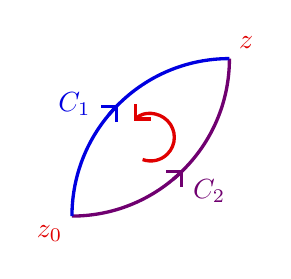
\begin{tikzpicture}
			\coordinate (O);
			\coordinate (A) at (2,2);
			\coordinate (C) at ({2+2*cos(145)},{2*sin(145)});
			\coordinate (D) at ({2*cos(-45)},{2+2*sin(-45)});
			\draw (O) node[below left,second] {$z_0$};
			\draw (A) node[above right,second] {$z$};
			\draw (C) node[above left,main] {$C_1$};
			\draw (D) node[below right,third] {$C_2$};
			\begin{scope}[cstcurve]
				\draw[third] (A) arc(0:-90:2);
				\draw[third,cstwra] ({2*cos(-50)},{2+2*sin(-50)}) arc(-50:-45:2);
				\draw[main] (O) arc(180:90:2);
				\draw[main,cstwra] ({2+2*cos(140)},{2*sin(140)}) arc(140:135:2);
				\draw[second,cstwla,visible on=<2->] ({1+0.3*cos(135)},{1+0.3*sin(135)}) arc(135:-110:0.3);
			\end{scope}
		\end{tikzpicture}
	\end{center}
\end{frame}


\begin{frame}{积分路径无关的函数特点}
	\onslide<+->
	上一节中我们计算了 $f(z)=z,\Re z,\dfrac1{z-z_0}$ 的积分.
	\onslide<+->
	其中
	\begin{itemize}
		\item $f(z)=z$ 处处解析, 积分只与起点终点有关 (闭路积分为零);
		\item $f(z)=\dfrac1{z-z_0}$ 有奇点 $z_0$, 沿绕 $z_0$ 闭路的积分非零;
		\item $f(z)=\Re z$ 处处不解析, 积分与路径有关 (闭路积分可能非零).
	\end{itemize}
	\onslide<+->
	由此可见函数沿闭路积分为零,
	\onslide<+->
	与函数在闭路内部是否解析有关.
\end{frame}


\begin{frame}{柯西-古萨基本定理: 推导}
	\onslide<+->
	设 $C$ 是一条闭路, $D$ 是其内部区域.
	\onslide<+->
	设 \emph{$f(z)$ 在闭区域 $\ov D=D\cup C$ 上解析},
	\onslide<+->
	即存在区域 $B\supseteq\ov D$ 使得 $f(z)$ 在 $B$ 上解析.

	\onslide<+->
	为了简便假设 $f'(z)$ 连续,
	\onslide<+->
	则
	\[\oint_Cf(z)\diff z=\oint_C(u\diff x-v\diff y)
	+i\oint_C(v\diff x+u\diff y).\]
	\onslide<+->
	由格林公式和C-R方程可知
	\[\oint_Cf(z)\diff z=-\iint_D(v_x+u_y)\diff x\diff y
	+i\iint_D(u_x-v_y)\diff x\diff y=0.\]
	\onslide<+->
	也可以从
	\[\oint_Cf(z)\diff z=-\iint_D\frac{\partial f}{\partial \ov z}\diff z\diff \ov z=2i\iint_D\frac{\partial f}{\partial \ov z}\diff x\diff y=0\]
	看出.
\end{frame}


\begin{frame}{柯西-古萨基本定理}
	\onslide<+->
	\begin{second}{柯西-古萨基本定理}
	设 $f(z)$ 在闭路 $C$ 上连续, $C$ 内部解析, 则 $\displaystyle\oint_Cf(z)\diff z=0$.
	\end{second}

	\onslide<+->
	\begin{corollary}
	设 $f(z)$ 在\alert{单连通域} $D$ 内解析, $C$ 是 $D$ 内一条闭合曲线, 则 $\displaystyle\oint_Cf(z)\diff z=0$.
	\end{corollary}
	\onslide<+->
	这里的闭合曲线可以不是闭路.

	% \onslide<+->
	% 这是因为即使不是简单曲线也可以拆分为一些简单曲线.
	% \onslide<4->
	% \begin{center}
	% 	\begin{tikzpicture}
	% 		\draw[cstcurve,main,smooth,domain=-45:-15] plot({3*sqrt(cos(2*\x))*cos(\x)},{3*sqrt(cos(2*\x))*sin(\x)});
	% 		\draw[cstcurve,main,smooth,domain=-20:45,cstwla] plot({3*sqrt(cos(2*\x))*cos(\x)},{3*sqrt(cos(2*\x))*sin(\x)});
	% 		\draw[cstcurve,main,smooth,domain=-45:-15] plot({-2*sqrt(cos(2*\x))*cos(\x)},{2*sqrt(cos(2*\x))*sin(\x)});
	% 		\draw[cstcurve,main,smooth,domain=-20:45,cstwla] plot({-2*sqrt(cos(2*\x))*cos(\x)},{2*sqrt(cos(2*\x))*sin(\x)});
	% 		\draw[cstcurve,second,cstwla,ultra thick] (1.05,0.35) arc (135:-135:0.5);
	% 		\draw[cstcurve,third,cstwla,ultra thick] (-0.75,-0.25) arc (315:45:0.3535);
	% 	\end{tikzpicture}
	% \end{center}
\end{frame}


\begin{frame}{典型例题: 柯西-古萨基本定理计算积分}
	\onslide<+->
	\begin{example}
		求 $\displaystyle\oint_{|z|=1}\frac1{2z-3}\diff z$.
	\end{example}

	\onslide<+->
	\begin{solution}
		由于 $\dfrac1{2z-3}$ 在 $|z|\le 1$ 上解析,
		\onslide<+->{因此由柯西-古萨基本定理 $\displaystyle \oint_{|z|=1}\frac1{2z-3}\diff z=0$.}
	\end{solution}

	\onslide<+->
	\begin{exercise}
		\begin{enumerate}
			\item $\displaystyle\oint_{|z-2|=1}\frac1{z^2+z}\diff z=$\fillblankframe{$0$}.
			\item 求 $\displaystyle\oint_{|z|=2}\dfrac{\sin z}{|z|}\diff z=$\fillblankframe{$0$}.
		\end{enumerate}
	\end{exercise}
\end{frame}


\begin{frame}{例: 柯西-古萨基本定理计算积分}
	\onslide<+->
	\begin{example}
		求 $\displaystyle\oint_C\frac1{z(z^2+1)}\diff z$, 其中 $C:|z-i|=\dfrac12$.
	\end{example}

	\onslide<+->
	\begin{solution}
		注意到 $\dfrac1{z(z^2+1)}=\dfrac1z-\dfrac12\left(\dfrac1{z+i}+\dfrac1{z-i}\right)$.
		\onslide<+->{由于 $\dfrac1z,\dfrac1{z+i}$ 在 $|z-i|\le\dfrac12$ 上解析,
		}\onslide<+->{因此由柯西-古萨基本定理
			\[\oint_C\frac1z\diff z
			=\oint_C\frac1{z+i}\diff z=0,\]
		}\onslide<+->{
			\[\oint_C\frac1{z(z^2+1)}\diff z
			=-\half\oint_C\frac1{z-i}\diff z=-\pi i.\]}
	\end{solution}
\end{frame}


\subsection{复合闭路定理}

\begin{frame}{多连通域边界与复合闭路}
	\onslide<+->
	设 $C_0,C_1,\dots,C_n$ 是 $n+1$ 条简单闭曲线, $C_1,\dots,C_n$ 每一条都包含在其它闭路的外部, 而且它们都包含在 $C_0$ 的内部.
	\onslide<+->
	这样它们围成了一个多连通区域 $D$, 它的边界称为一个\emph{复合闭路} \[C=C_0+C_1^-+\cdots+C_n^-.\]
	\onslide<+->
	沿着 $C$ 前进的点, $D$ 总在它的左侧,所以这就是它的正方向.
	\onslide<1->
	\begin{center}
		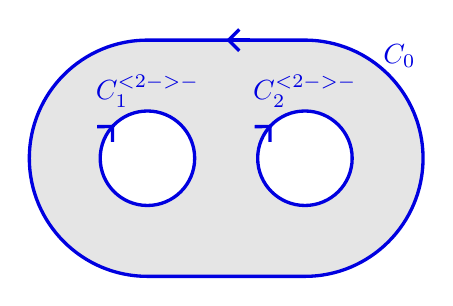
\begin{tikzpicture}
			\fill[cstfill,visible on=<2->,rounded corners=15mm] (-2.5,-1.5) rectangle (2.5,1.5);
			\draw[cstcurve,main,rounded corners=15mm] (-2.5,-1.5) rectangle (2.5,1.5);
			\fill[cstcurve,white,visible on=<2->] (1,0) circle(0.6);
			\fill[cstcurve,white,visible on=<2->] (-1,0) circle(0.6);
			\draw[cstcurve,main] (1,0) circle(0.6);
			\draw[cstcurve,main] (-1,0) circle(0.6);
			\draw[cstcurve,main,domain=85:90,cstwra,visible on=<2->] plot (.3,1.5)--(0,1.5);
			\draw[cstcurve,main,domain=135:140,cstwla,visible on=<2->] plot ({1+0.6*cos(\x)}, {0.6*sin(\x)});
			\draw[cstcurve,main,domain=135:140,cstwla,visible on=<2->] plot ({-1+0.6*cos(\x)}, {0.6*sin(\x)});
			\draw
				(2.2,1.3) node[main] {$C_0$}
				(-1,0.85) node[main] {$C_1^{\visible<2->-}$}
				(1,0.85) node[main] {$C_2^{\visible<2->-}$};
		\end{tikzpicture}
	\end{center}
\end{frame}


\begin{frame}{复合闭路定理}
	\onslide<+->
	\begin{second}{复合闭路定理}
		设 $f(z)$ 在复合闭路 $C=C_0+C_1^-+\cdots+C_n^-$ 及其所围成的多连通区域内解析, 则
		\[\oint_{C_0}f(z)\diff z=
		\oint_{C_1}f(z)\diff z+\cdots+\oint_{C_n}f(z)\diff z.\]
	\end{second}
	\onslide<+->
	事实上, 复合闭路定理和柯西-古萨基本定理可以看成一个定理的两种情形: 
	\onslide<+->
	设 $C$ 是一个闭路或复合闭路, 若 $f(z)$ 在 $C$ 及其围成的区域(单连通或多连通)内解析, 则 $\displaystyle\oint_Cf(z)\diff z=0$.
\end{frame}



\begin{frame}{复合闭路定理: 注记}
	\onslide<+->
	在实际应用中, 如果被积函数 $f(z)$ 在(复合)闭路 $C$ 的内部有有限多个奇点 $z_1,\dots,z_k$.
	\onslide<+->
	那么我们可以在 $C$ 内部(围成的区域)构造闭路 $C_1,\dots,C_k$, 使得每个 $C_j$ 内部只包含一个奇点 $z_j$.
	\onslide<+->
	这样, 内部含多个奇点的情形就可以化成内部只含一个奇点的情形. 最后将这些闭路上的积分相加即可.
	\onslide<1->
	\begin{center}
		\begin{tikzpicture}
			\draw[cstcurve,main,rounded corners=10mm] (-2.2,-1.2) rectangle (2.2,1.2);
			\draw[cstcurve,second,visible on=<2->] (1,0) circle(0.4);
			\draw[cstcurve,second,visible on=<2->] (0,0) circle(0.4);
			\draw[cstcurve,second,visible on=<2->] (-1,0) circle(0.4);
			\fill[cstdot,second] (1,0) circle;
			\fill[cstdot,second] (0,0) circle;
			\fill[cstdot,second] (-1,0) circle;
			\draw
				(-1,-0.25) node[second] {$z_1$}
				(0,-0.25) node[second] {$z_2$}
				(1,-0.25) node[second] {$z_3$}
				(2.2,1.1) node[main] {$C$}
				(-1,0.65) node[second,visible on=<2->] {$C_1$}
				(0,0.65) node[second,visible on=<2->] {$C_2$}
				(1,0.65) node[second,visible on=<2->] {$C_3$};
		\end{tikzpicture}
	\end{center}
\end{frame}


\begin{frame}{复合闭路定理: 注记}
	\onslide<+->
	此外, 从复合闭路定理还可以看出, 在计算积分 $\displaystyle \oint_C f(z)\diff z$ 时, $C$ 的具体形状无关紧要, 只要其内部奇点不变, $C$ 可以任意变形.
	\onslide<+->
	因为我们总可以选择一个包含这些奇点的闭路 $C'$, 使得 $C'$ 包含在 $C$ 及其变形后的闭路内部. 这样它们的积分自然都和 $C'$ 上的积分相同.
	\onslide<+->
	这里即使 $C$ 是复合闭路也是可以自由变形的.
	\onslide<1->
	\begin{center}
		\begin{tikzpicture}
			\draw[cstcurve,main,rounded corners=10mm] (-2.2,-1.2) rectangle (2.2,1.2);
			\draw[cstcurve,third] (0,0) circle(1.2 and 2.2);
			\draw[cstcurve,second,visible on=<2->] (0,0) circle(1);
			\fill[cstdot,second] (.7,0.2) circle;
			\fill[cstdot,second] (0,-0.4) circle;
			\fill[cstdot,second] (-.5,0.1) circle;
			\draw
				(2,1.4) node[main] {$C_1$}
				(-1.1,1.8) node[third] {$C_2$}
				(-.4,0.65) node[second,visible on=<2->] {$C'$};
		\end{tikzpicture}
	\end{center}
\end{frame}


\begin{frame}{复合闭路定理}
	\onslide<+->
	\begin{proof}
		以曲线 $\gamma_1,\gamma_2,\dots,\gamma_{n+1}$ 把 $C_0,C_1,\dots,C_n$ 连接起来, 则它们把区域 $D$ 分成了两个单连通域 $D_1,D_2$.
		\onslide<+->{对 $D_1$ 和 $D_2$ 的边界应用柯西-古萨基本定理并相加, 则 $\gamma_i$ 对应的部分正好相互抵消,
		}\onslide<+->{因此
			\[\oint_{C_0}f(z)\diff z-
		\oint_{C_1}f(z)\diff z-\cdots-\oint_{C_n}f(z)\diff z=0.\]
		}\onslide<+->{于是定理得证.\qedhere}
		\vspace{-1.7\baselineskip}
		\onslide<1->
		\begin{center}
			\begin{tikzpicture}[scale=.9]
				\fill[cstcurve,cstfill] (0,0) circle(2.5 and 1.5);
				\fill[cstcurve,white] (1,0) circle(0.6);
				\fill[cstcurve,white] (-1,0) circle(0.6);

				\draw[cstcurve,main,domain=0:90,cstwra] plot ({2.5*cos(\x)}, {1.5*sin(\x)});
				\draw[cstcurve,main,domain=85:180] plot ({2.5*cos(\x)}, {1.5*sin(\x)});
				\draw[cstcurve,second,domain=180:270,cstwra] plot ({2.5*cos(\x)}, {1.5*sin(\x)});
				\draw[cstcurve,second,domain=265:360] plot ({2.5*cos(\x)}, {1.5*sin(\x)});

				\draw[cstcurve,main,domain=0:140] plot ({1+0.6*cos(\x)}, {0.6*sin(\x)});
				\draw[cstcurve,main,domain=135:180,cstwla] plot ({1+0.6*cos(\x)}, {0.6*sin(\x)});
				\draw[cstcurve,second,domain=180:320] plot ({1+0.6*cos(\x)}, {0.6*sin(\x)});
				\draw[cstcurve,second,domain=315:360,cstwla] plot ({1+0.6*cos(\x)}, {0.6*sin(\x)});

				\draw[cstcurve,main,domain=0:140] plot ({-1+0.6*cos(\x)}, {0.6*sin(\x)});
				\draw[cstcurve,main,domain=135:180,cstwla] plot ({-1+0.6*cos(\x)}, {0.6*sin(\x)});
				\draw[cstcurve,second,domain=180:320] plot ({-1+0.6*cos(\x)}, {0.6*sin(\x)});
				\draw[cstcurve,second,domain=315:360,cstwla] plot ({-1+0.6*cos(\x)}, {0.6*sin(\x)});

				\draw
					(2,1.3) node[main] {$C_0$}
					(-1,0.85) node[main] {$C_1^-$}
					(1,0.85) node[main] {$C_2^-$}
					(-2,-0.3) node {$\gamma_1$}
					(0,-0.3) node {$\gamma_2$}
					(2,-0.3) node {$\gamma_3$};
				\draw[cstcurve] (-2.5,0)--(-1.6,0);
				\draw[cstcurve] (-0.4,0)--(0.4,0);
				\draw[cstcurve] (1.6,0)--(2.5,0);
				\draw[cstcurve,thick,main,visible on=<2->] (-2.5,0.025)--(-1.6,0.025);
				\draw[cstcurve,thick,second,visible on=<2->] (-2.5,-0.025)--(-1.6,-0.025);
				\draw[cstcurve,thick,main,visible on=<2->] (-0.4,0.025)--(0.4,0.025);
				\draw[cstcurve,thick,second,visible on=<2->] (-0.4,-0.025)--(0.4,-0.025);
				\draw[cstcurve,thick,main,visible on=<2->] (1.6,0.025)--(2.5,0.025);
				\draw[cstcurve,thick,second,visible on=<2->] (1.6,-0.025)--(2.5,-0.025);
			\end{tikzpicture}
		\end{center}
		\vspace{-\baselineskip}
	\end{proof}
\end{frame}


\begin{frame}{例: 复合闭路定理的应用}
	\onslide<+->
	\begin{example}
		证明对于任意闭路 $C$, $\displaystyle\int_C(z-a)^n\diff z=0$, $n\neq -1$ 为整数.
	\end{example}

	\onslide<+->
	\begin{proof}
		\begin{enumerate}
			\item 如果 $a$ 不在 $C$ 的内部, 则 $(z-a)^n$ 在 $C$ 及其内部解析.
			\onslide<+->{%
				由柯西-古萨基本定理, $\displaystyle\int_C(z-a)^n\diff z=0$.
			}
			\item 如果 $a$ 在 $C$ 的内部, 则在 $C$ 的内部取一个以 $a$ 为圆心的圆周 $C_1$.
			\onslide<+->{%
				由复合闭路定理以及上一节的结论
				\[
					\int_C(z-a)^n\diff z=\int_{C_1}(z-a)^n\diff z=0.\qedhere
				\]
			}
			\vspace{-\baselineskip}
		\end{enumerate}
	\end{proof}
\end{frame}


\begin{frame}{例: 复合闭路定理的应用}
	\onslide<+->
	同理, 由复合闭路定理和上一节的结论可知当 $a$ 在 $C$ 的内部且 $n=-1$ 时积分为 $2\pi i$.
	\onslide<+->
	\begin{theorem@}
		当 $a$ 在 $C$ 的内部时,
		\[\oint_C\frac{\diff z}{(z-a)^{n+1}}=\begin{cases}2\pi i,&n=0;\\0,&n\neq 0.\end{cases}\]
	\end{theorem@}
\end{frame}


\begin{frame}{例: 复合闭路定理的应用}
	\beqskip{4pt}
	\onslide<+->
	\begin{example}
		\begin{minipage}{.6\textwidth}
			求 $\displaystyle\int_\Gamma\frac{2z-1}{z^2-z}\diff z$, 其中 $\Gamma$ 是由 $2\pm i,-2\pm i$ 形成的矩形闭路.
		\end{minipage}
		\begin{minipage}{.36\textwidth}
			\begin{tikzpicture}
				\draw[cstaxis] (-2.5,0)--(2.5,0);
				\draw[cstaxis] (0,-1)--(0,1);
				\draw[cstcurve,cstwra,main] (-1,-0.7)--(-0.5,-0.7);
				\draw[cstcurve,cstwra,second,visible on=<3->] (-0.4,0) arc(180:225:0.4);
				\draw[cstcurve,cstwra,second,visible on=<3->] (0.6,0) arc(180:225:0.4);
				\draw[cstcurve,second,visible on=<3->] (0,0) circle (0.4);
				\draw[cstcurve,second,visible on=<3->] (1,0) circle (0.4);
				\fill[cstdot,third,visible on=<2->] (1,0) circle;
				\fill[cstdot,third,visible on=<2->] (0,0) circle;
				\draw[cstcurve,main] (-2,-0.7) rectangle (2,0.7);
				\draw
					(-0.6,0.4) node[second,visible on=<3->] {$C_1$}
					(1.6,0.4) node[second,visible on=<3->] {$C_2$}
					(-1,-0.5) node[main] {$\Gamma$};
			\end{tikzpicture}
		\end{minipage}
	\end{example}
	\onslide<+->
	\begin{solution}
		函数 $\dfrac{2z-1}{z^2-z}$ 在 $\Gamma$ 内有两个奇点 $z=0,1$.
		\onslide<+->{%
			设 $C_1,C_2$ 如图所示,
		}\onslide<+->{%
			由复合闭路定理
			\begin{align*}
				&\oint_\Gamma\frac{2z-1}{z^2-z}\diff z
				=\oint_{C_1}\frac{2z-1}{z^2-z}\diff z+\oint_{C_2}\frac{2z-1}{z^2-z}\diff z\\
				\visible<+->{=}&\visible<.->{\oint_{C_1}\frac1z\diff z+\oint_{C_1}\frac1{z-1}\diff z
				+\oint_{C_2}\frac1z\diff z+\oint_{C_2}\frac1{z-1}\diff z}\\
				\visible<+->{=}&\visible<.->{2\pi i+0+0+2\pi i=4\pi i.}
			\end{align*}
		}\vspace{-\baselineskip}
	\end{solution}
	\endgroup
\end{frame}


\begin{frame}{例: 复合闭路定理的应用}
	\onslide<+->
	\begin{example}
		求 $\displaystyle\int_\Gamma\frac{e^z}z\diff z$, 其中 $\Gamma=C_1+C_2^-$, $C_1:|z|=2, C_2:|z|=1$.
		\vspace{-.8\baselineskip}
		\begin{center}
			\begin{tikzpicture}[scale=.8]
				\filldraw[cstcurve,main,cstfill] (0,0) circle (1.5);
				\draw[cstcurve,main,cstwla] (-1.06,1.06) arc(135:90:1.5);
				\filldraw[cstcurve,second,fill=white] (0,0) circle (0.75);
				\draw[cstcurve,second,cstwra] (-0.75,0) arc(180:130:0.75);
				\draw
					(-1.6,0.8) node[main] {$C_1$}
					(0.8,-0.7) node[second] {$C_2^-$};
				\draw[cstaxis] (-1.8,0)--(1.8,0);
				\draw[cstaxis] (0,-1.8)--(0,1.8);
			\end{tikzpicture}
		\end{center}
		\vspace{-.8\baselineskip}
	\end{example}
	\onslide<+->
	\begin{solution}
		函数 $\dfrac{e^z}z$ 在 $C_1,C_2$ 围城的圆环域内解析.
		\onslide<+->{由复合闭路定理可知 $\displaystyle\int_\Gamma\frac{e^z}z\diff z=0$.}
	\end{solution}
\end{frame}



\section{原函数和不定积分}

\subsection{原函数}

\begin{frame}{原函数的存在性}
	\onslide<+->
	设 $f(z)$ 在单连通域 $D$ 内解析, $C$ 是 $D$ 内一条起于 $z_0$ 终于 $z$ 的曲线.
	\onslide<+->
	由柯西-古萨基本定理可知, 积分 $\displaystyle\int_Cf(\zeta)\diff \zeta$ 与路径无关, 只与 $z_0,z$ 有关.
	\onslide<+->
	因此我们也将其记为 $\displaystyle\int_{z_0}^zf(\zeta)\diff\zeta$.

	\onslide<+->
	对于任意固定的 $z_0\in D$, 定义
	\[F(z)=\int_{z_0}^zf(\zeta)\diff\zeta.\]
\end{frame}


\begin{frame}{原函数的存在性}
	\beqskip{0pt}
	\onslide<+->
	\begin{theorem}
		$F(z)$ 是 $D$ 内的解析函数, 且 $F'(z)=f(z)$.
	\end{theorem}
	\onslide<+->
	\begin{solution}[证明]
		\begin{center}
			\begin{tikzpicture}
				\fill[cstcurve,main,rounded corners=0.5cm,cstfill] (-2.5,-0.8) rectangle (2,1);
				\draw[cstcurve,main] (0,0) circle(0.7);
				\draw[cstcurve,third] (-2,0)to [bend left](0,0);
				\draw[cstcurve,third,visible on=<2->] (0,0)--(0.4,0.4);
				\fill[cstdot,third] (-2,0) circle;
				\fill[cstdot,third] (0,0) circle;
				\fill[cstdot,third,visible on=<2->] (0.4,0.4) circle;
				\draw
					(-2,-0.3) node[third] {$z_0$}
					(0,-0.3) node[third] {$z$}
					(1.1,0.7) node[third,visible on=<2->] {$z+\Delta z$};
			\end{tikzpicture}
		\end{center}
		以 $z$ 为中心作一包含在 $D$ 内的圆 $K$,
		\onslide<+->{%
			取 $|\Delta z|$ 小于 $K$ 的半径.
		}\onslide<+->{%
			那么
			\[
				F(z+\Delta z)-F(z)=\int_{z_0}^{z+\Delta z}f(\zeta)\diff\zeta-\int_{z_0}^zf(\zeta)\diff\zeta
				\visible<+->{=\int_z^{z+\Delta z}f(\zeta)\diff\zeta.}
			\]
		}\onslide<+->{%
			容易知道
			$\displaystyle\int_z^{z+\Delta z}f(z)\diff\zeta=f(z)\int_z^{z+\Delta z}\diff\zeta=f(z)\Delta z$.
		}\onslide<+->{%
			我们需要比较上述两个积分, 其中 $z$ 到 $z+\Delta z$ 取直线.
		}
	\end{solution}
	\endgroup
\end{frame}


\begin{frame}{原函数的存在性}
	\onslide<+->
	\begin{proof}[续证]
		由于 $f(z)$ 解析, 因此连续.
		\onslide<+->{$\forall\varepsilon>0,\exists\delta>0$ 使得当 $|\zeta-z|<\delta$ 时, $z$ 落在 $K$ 中且 $|f(\zeta)-f(z)|<\varepsilon$.
		}\onslide<+->{当 $|\Delta z|<\delta$ 时, 由长大不等式
			\begin{align*}
			\abs{\frac{F(z+\Delta z)-F(z)}{\Delta z}-f(z)}
			&\visible<+->{=\abs{\int_z^{z+\Delta z}\frac{f(\zeta)-f(z)}{\Delta z}\diff \zeta}}\\
			&\visible<+->{\le\frac{\varepsilon}{|\Delta z|}\cdot|\Delta z|=\varepsilon.}
			\end{align*}
		}\onslide<+->{由于 $\varepsilon$ 是任意的, 因此
		\[f(z)=\lim_{\Delta z\to 0}\frac{F(z+\Delta z)-F(z)}{\Delta z}=F'(z).\qedhere\]}
	\end{proof}
\end{frame}


\subsection{牛顿-莱布尼兹定理}

\begin{frame}{牛顿-莱布尼兹定理}

	\onslide<+->
	如果 $D$ 上的解析函数 $G(z)$ 满足 $G'(z)=f(z)$, 则称 $G(z)$ 是 $f(z)$ 的一个\emph{原函数}.
	\onslide<+->
	由于导函数为 $0$ 的解析函数只能是常值函数,
	\onslide<+->
	因此 $\displaystyle G(z)=\int_{z_0}^zf(\zeta)\diff \zeta+C$.
	\onslide<+->
	我们称之为 $f(z)$ 的\emph{不定积分}, 记为 \emph{$\displaystyle\int f(z)\diff z$}.

	\onslide<+->
	\begin{second}{复变函数积分计算方法II}
		设 $f(z)$ 在单连通区域 $D$ 上解析, $z_1$ 至 $z_2$ 的积分路径落在 $D$ 内, 则
		\[
			\int_{z_1}^{z_2}f(z)\diff z=F(z)\Big|_{z_1}^{z_2}=F(z_2)-F(z_1),\]
		其中 $F(z)$ 是 $f(z)$ 的一个原函数.
	\end{second}

	\onslide<+->
	复变函数和实变函数的牛顿-莱布尼兹定理的差异在哪呢?
	\onslide<+->
	复变情形要求是\alert{单连通区域上解析函数}, 实变情形要求是\alert{闭区间上连续函数}.
\end{frame}


\begin{frame}{典型例题: 利用原函数求积分}
	\onslide<+->
	\begin{example}
		求 $\displaystyle\int_{z_0}^{z_1}z\diff z$.
	\end{example}

	\onslide<+->
	\begin{solution}
		由于 $f(z)=z$ 处处解析,
		\onslide<+->{%
			且 $\displaystyle\int z\diff z=\half  z^2+C$,
		}\onslide<+->{%
			因此
			\[
				\int_{z_0}^{z_1}z\diff z=\half z^2\big|_{z_0}^{z_1}=\half (z_1^2-z_0^2).
			\]
		}\vspace{-.5\baselineskip}
	\end{solution}
	\onslide<+->
	因此之前的例子中 $\displaystyle\int_0^{3+4i}z\diff z=-\frac72+12i$, 无论从 $0$ 到 $3+4i$ 的路径如何.
\end{frame}


\begin{frame}{典型例题: 利用原函数求积分}
	\onslide<+->
	\begin{example}
		求 $\displaystyle\int_0^{\pi i}z\cos z^2\diff z$.
	\end{example}

	\onslide<+->
	\begin{solution}
		由于 $f(z)=z\cos z^2$ 处处解析,
		\onslide<+->{%
			且
			\[
				\int z\cos z^2\diff z=\half\int \cos z^2\diff z^2=\half\sin z^2+C,
			\]
		}\onslide<+->{%
			因此
			\[
				\int_0^{\pi i}z\cos z^2\diff z=\half\sin z^2\big|_0^{\pi i}=-\half\sin \pi^2.
			\]
		}\vspace{-.5\baselineskip}
	\end{solution}

	\onslide<+->
	这里我们使用了\alert{凑微分法}.
\end{frame}


\begin{frame}{典型例题: 利用原函数求积分}
	\onslide<+->
	\begin{example}
		求 $\displaystyle\int_0^i z\cos z\diff z$.
	\end{example}

	\onslide<+->
	\begin{solution}
		由于 $f(z)=z\cos z$ 处处解析,
		\onslide<+->{%
			且
			\[
				\int z\cos z\diff z
				=\int z\diff(\sin z)
				=z\sin z-\int \sin z\diff z
				\visible<+->{=z\sin z+\cos z+C,}
			\]
		}\onslide<+->{%
			因此
			\[
				\int_0^i z\cos z\diff z
				=(z\sin z+\cos z)\big|_0^i
				\visible<+->{=i\sin i+\cos i-1=e^{-1}-1.}
			\]
		}\vspace{-.5\baselineskip}
	\end{solution}
	\onslide<+->
	这里我们使用了\alert{分部积分法}.
\end{frame}


\begin{frame}{典型例题: 利用原函数求积分}
	\onslide<+->
	\begin{example}
		求 $\displaystyle\int_1^{1+i} z e^z\diff z$.
	\end{example}
	\onslide<+->
	\begin{solution}
		由于 $f(z)=ze^z$ 处处解析,
		\onslide<+->{%
			且 $\displaystyle\int z e^z\diff z=\int z\diff e^z=ze^z-\int e^z\diff z=(z-1)e^z+C$,
		}\onslide<+->{%
			因此 $\displaystyle \int_1^{1+i} z e^z\diff z=(z-1)e^z\big|_1^{1+i}
			\visible<+->{=ie^{1+i}=e(-\sin 1+i\cos 1)}$.
		}
	\end{solution}
	\onslide<+->
	\begin{exercise}
		求 $\displaystyle\int_0^1 z\sin z\diff z=$\fillblankframe[4cm]{$\sin 1-\cos 1$}.
	\end{exercise}
\end{frame}


\begin{frame}{典型例题: 利用原函数求积分}
	\beqskip{0pt}
	\onslide<+->
	\begin{example}
		求 $\displaystyle\int_C(2z^2+8z+1)\diff z$, 其中 $C$ 是摆线
		$\displaystyle\begin{cases}
		x=a(\theta-\sin\theta),& \\ y=a(1-\cos\theta),
		\end{cases} 0\le \theta\le 2\pi.$
		\vspace{-\baselineskip}
		\begin{center}
			\begin{animateinline}[width=9cm]{10}
				\begin{tikzpicture}
					\draw[cstaxis, thick](-1.5,0)--(7.5,0);
					\draw[cstaxis, thick](0,0)--(0,2.5);
					\draw[cstcurve,main,smooth,domain=0:360] plot ({1*(pi/180*\x-sin(\x))},{1*(1-cos(\x))});
				\end{tikzpicture}
				\newframe
				\multiframe{37}{r=0+10}{
					\begin{tikzpicture}
						\draw[cstaxis, thick](-1.5,0)--(7.5,0);
						\draw[cstaxis, thick](0,0)--(0,2.5);
						\draw[cstcurve,second] ({1*(pi/180*\r)},1) circle (1);
						\fill[cstdot,main] ({1*(pi/180*\r-sin(\r))},{1*(1-cos(\r))}) circle;
						\draw[cstcurve,main,smooth,domain=0:360] plot ({1*(pi/180*\x-sin(\x))},{1*(1-cos(\x))});
					\end{tikzpicture}
				}
			\end{animateinline}
		\end{center}
	\end{example}
	\onslide<+->
	\begin{solution}
		由于 $f(z)=2z^2+8z+1$ 处处解析,
		\onslide<+->{%
			因此
			\[
				\text{原积分}=\int_0^{2\pi a}(2z^2+8z+1)\diff z
				\visible<+->{=\left(\frac23z^3+4z^2+z\right)\bigg|_0^{2\pi a}=\frac{16}3\pi^3a^3+16\pi^2a^2+2\pi a.}
			\]
		}
	\end{solution}
	\endgroup
\end{frame}


\begin{frame}{典型例题: 利用原函数求积分}
	\beqskip{3pt}
	\onslide<+->
	\begin{example}
		设 $C$ 为沿着 $|z|=1$ 从 $1$ 到 $i$ 的逆时针圆弧, 求 $\displaystyle\int_C\frac{\ln(z+1)}{z+1}\diff z$.
	\end{example}

	\onslide<+->
	\begin{solution}
		函数 $f(z)=\dfrac{\ln(z+1)}{z+1}$ 在单连通区域 $\Re z>-1$ 内解析.
		\onslide<+->{%
			\[\int\frac{\ln(z+1)}{z+1}\diff z
			=\int\ln(z+1)\diff[\ln(z+1)]=\half\ln^2(z+1)+C.\]
		}\onslide<+->{%
			因此
			\begin{align*}
				\int_C\frac{\ln(z+1)}{z+1}\diff z&=\half\ln^2(z+1)\big|_1^i
				\visible<+->{=\half\left[\ln^2(1+i)-\ln^22\right]}\\
				&\visible<+->{=\half\biggl(\Bigl(\ln\sqrt2+\frac\pi4i\Bigr)^2-\ln^22\biggr)
				=-\frac{\pi^2}{32}-\frac38\ln^22+\frac{\pi\ln2}{8}i.}
			\end{align*}
		}
	\end{solution}
	\endgroup
\end{frame}



\end{document}

授课进度:

1 线性映射、矩阵、矩阵的线性运算
2 矩阵的乘法、幂和转置
3 行列式的定义和性质
4 拉普拉斯变换和行列式的计算
5 方阵的伴随矩阵和逆矩阵的定义和形式
6 逆矩阵的性质和克拉默法则
7 分块矩阵、初等矩阵和矩阵等价
8 初等变换解矩阵方程、向量组的线性表示、线性相关与线性无关
9 线性相关与线性无关的性质、极大线性无关组
10 矩阵的秩
11 标准正交基、齐次线性方程组
12 线性方程组
13 
14
15
16
17
18




一次20~25页

